\documentclass[lncs]{mmiss}

%\input{prelude.tex}
%% use of LaTeX packages
\usepackage{graphicx}
\usepackage{xspace}
\usepackage{verbatim}
\usepackage{proof-trees,picinpar}




%% new Categories; to be predefined
%% -- should be DefineCategory instead of newcommand everywhere
%Family
\newcommand{\Typewriter}[1]{\texttt{#1}}

%%\newcommand{\Roman}[1]{\textrm{#1}} already defined

\newcommand{\SansSerif}[1]{\textsf{#1}}

%Form
\newcommand{\SmallCaps}[1]{\textsc{#1}}
\newcommand{\Italics}[1]{\textit{#1}}
\newcommand{\Slanted}[1]{\textsl{#1}}
\newcommand{\Upright}[1]{\textup{#1}}
%Series
\newcommand{\Bold}[1]{\textbf{#1}}

\newcommand{\NoBold}[1]{\textmd{#1}}


\newcommand{\Underline}[1]{\underline{#1}}


\newcommand{\Hidden}[1]{}

\newcommand{\Emphasis}[1]{\emph{#1}}
\newcommand{\Special}[1]{\SansSerif{#1}}  %redefine as Roman for Slides
\newcommand{\GivenName}[1]{\SmallCaps{#1}}
\newcommand{\SourceText}[1]{\Typewriter{#1}}

\def\Source{\small\verbatim} %to be used like verbatim, i.e. with begin and end
\def\endSource{\endverbatim} 



%%some MMiSS commands, simulated for the moment; ignore definition

        \newcommand{\Declare}[2]{\newcommand{#1}{#2}}
        \newcommand{\DeclImport}[2]{\Declare{#1}{#2}}
        \newcommand{\DeclClass}[4]{\newcommand{#4}{\Special{#2}}}    
        %\DeclClass{<Name>}{<ClassText>}{<Superclass>}{\<Name>}

        \newcommand{\DeclObject}[4]{\newcommand{#4}{\Special{#2}}} 
        %\DeclObject{<Name>}{<ObjectText>}{<Class>}{\<Name>} 

        \newcommand{\DeclRelation}[6][*-*]{\newcommand{#6}[2]{\Special{#3}}}      
        %\DeclRelation[<Functionality>]{<Name>}{<RelationText>}{<SourceClass>}{<TargetClass>}{\<Name>} 
        %% note that \<Name> declares just the <RelationText>, with 2 parameters; it can be used as "A \R{}{} B"
        %% but not yet in a binary fashion "\R{A}{B}" yielding A r B.

        \newcommand{\Define}[2]{\label{#1}{\Emphasis{#2}}}                             
        \newcommand{\DefClass}[2]{\label{#1}{\Emphasis{#2}}}                             
        \newcommand{\DefObject}[2]{\label{#1}{\Emphasis{#2}}}                             
        \newcommand{\DefRelation}[2]{\label{#1}{\Emphasis{#2{}{}}}}                             
        \newcommand{\Ref}[2]{#2}                       

        \newcommand{\Reference}[2]{#2 (see Sect.~\ref{#1}}                       


%% in this document, at the moment (since the MMiSS commands do not yet work properly)
%% we use an extra parameter at the end ("\Name", for "Name" as the first parameter)
%% that will go away in 2 weeks, for these commands:
%               \Define{Name}{\Name}
%   for         \Define{Name} ;
%               \Ref{Name}{\Name}
%   for         \Ref{Name} ;
%               \Reference{Name}{\Name}
%   for         \Reference{Name} ;
%               \DeclClass{<Name>}{<ClassText >}{<Superclass>}{\<Name>}
%   for         \DeclClass{<Name>}{<ClassText >}{<Superclass>} ;
%               \DeclObject{<Name>}{<ObjectText >}{<Class>}{\<Name>}
%   for         \DeclObject{<Name>}{<ObjectText >}{<Class>} ;
%               \DeclRelation[<Functionality>]{<Name>}{<RelationText>}{<SourceClass>}{<TargetClass>}{\<Name>} 
%   for         \DeclRelation[<Functionality>]{<Name>}{<RelationText>}{<SourceClass>}{<TargetClass>}
        
        
%% editing Categories (at the moment), to be replaced by MMiSS annotations; to be made empty in final paper
\newcommand{\MarginComment}[1]{\marginpar{\footnotesize\texttt{#1}}}
\newcommand{\RevisedBy}[1]{\MarginComment{Revised by: \\#1}}
\newcommand{\BKB}[1]{\MarginComment{BKB: #1}}
\newcommand{\CXL}[1]{\MarginComment{CXL: #1}}
\newcommand{\Authors}[1]{\MarginComment{Authors: #1}}
        

%% import of packages, simulated, and definition of ontology
%\input{mmiss-ontology.tex}
%% Simulation of import Ontology
%% should be proper DeclClass etc. instead, see below

%% simulate import of package Graph
\DeclImport{\Graph}{graph}
\DeclImport{\Node}{node}
\DeclImport{\Edge}{edge}
\DeclImport{\GraphVisualisation}{graph visualisation}

%% simulate import of package Algebra
\DeclImport{\TECS}{\GivenName{TeCS}}
\DeclImport{\Signature}{\Special{Signature}}
\DeclImport{\Algebra}{\Special{Algebra}}
\DeclImport{\Term}{\Special{Term}}
\DeclImport{\SigmaAlgebra}{\Special{$\Sigma$-algebra}}  

%% simulate import of package Haskell
\DeclImport{\Haskell}{\GivenName{Haskell}}

%% simulate import of package C
\DeclImport{\C}{\GivenName{C}}

%% simulate import of package Java
\DeclImport{\JAVA}{\GivenName{Java}}

%% simulate import of package CSP
\DeclImport{\CSP}{\GivenName{CSP}}

%% simulate import of package Casl
\DeclImport{\CoFI}{\GivenName{CoFI}}
\DeclImport{\CASL}{\GivenName{Casl}}
\DeclImport{\HOLCASL}{\GivenName{HOL/Casl}}
\DeclImport{\CATS}{\GivenName{CATS}}

%% simulate import of package Formats
\DeclImport\ASCII{\GivenName{ASCII}}
\DeclImport{\PDF}{\GivenName{PDF}}
\DeclImport{\HTML}{\GivenName{HTML}}
\DeclImport{\PS}{\GivenName{PostScript}}


%% simulate import of package XML
\DeclImport{\XML}{\GivenName{XML}}
\DeclImport{\XMLDocTypeDef}{document type definition}
\DeclImport{\DTD}{\GivenName{DTD}}
\DeclImport{\XMLEntityDef}{entity definition}
\DeclImport{\XMLElementDef}{element definition}
\DeclImport{\XMLAttribute}{attribute}


%% simulate import of package Emacs
\DeclImport{\Emacs}{\GivenName{Emacs}}
\DeclImport{\XEmacsEditor}{\GivenName{XEmacs} editor}
\DeclImport{\AUCTeX}{\GivenName{AUC\TeX}}

%% simulate import of package PowerPoint
\DeclImport{\PPT}{\GivenName{PowerPoint}}
\DeclImport{\CPoint}{\GivenName{CPoint}}

%% simulate import of package LaTeX
\DeclImport{\LaTeXEnvironment}{environment} 
\DeclImport{\LaTeXCommand}{command} 
\DeclImport{\PDFLaTeX}{\GivenName{PDF\-\LaTeX{}}}
\DeclImport{\PPower}{\GivenName{PPower4}} 
\DeclImport{\PauseLevel}{pause level} 
\DeclImport{\ProofLaTeX}{\GivenName{proof}} 


%% simulate import of package OmDoc
\DeclImport{\OpenMath}{\GivenName{OpenMath}}
\DeclImport{\MathML}{\GivenName{MathML}}
\DeclImport{\OMDoc}{\GivenName{OMDoc}}

%% simulate import of package ActiveMath
\DeclImport{\ActiveMath}{\GivenName{ActiveMath}}

%% simulate import of package WebAssign
\DeclImport{\WebAssign}{\GivenName{WebAssign}}



%%%%%%%%%%%%%%%%%%%%%%%%%%%%%%%%%%%%%%%%%%%%%%%%



%% declaration of Ontology for semantic document structuring

\DeclClass{Ontology}{ontology}{}{\Ontology} 
\DeclClass{OntologyStr}{Ontology}{Ontology}{\OntologyStr} 
        \DeclClass{OntologyClassStr}{OntologyClass}{OntologyStr}{\OntologyClassStr} 
        \DeclClass{OntologyObjectStr}{OntologyObject}{OntologyStr}{\OntologyObjectStr} 

        \DeclClass{OntologyRelationStr}{OntologyRelation}{OntologyStr}{\OntologyRelationStr} 


\DeclClass{DocStructuringOperation}{structuring operation}{}{\DocStructuringOperation}
%               % StructuralLink, SemanticRef neu definieren

        %% in the ontology of StructuralEntities, the Superclasses have to be inserted yet
        \DeclClass{StructuralEntities}{structural entities}{}{\StructuralEntities} 

                \DeclClass{GroupStr}{Group}{}{\GroupStr} 
                        \DeclClass{PackageStr}{Package}{}{\PackageStr} 

                        \DeclClass{SectionStr}{Section}{}{\SectionStr} 

                                \DeclRelation{Contains}{Contains}{SectionStr}{SectionStr}{\Contains}   
                                \DeclRelation{ReliesOn}{ReliesOn}{SectionStr}{SectionStr}{\ReliesOn}   
                        \DeclClass{ParagraphStr}{Paragraph}{}{\ParagraphStr} 

                                \DeclClass{AbstractStr}{Abstract}{}{\AbstractStr} 
                                \DeclClass{IntroductionStr}{Introduction}{}{\IntroductionStr} 
                                \DeclClass{SummaryStr}{Summary}{}{\SummaryStr} 

                        \DeclClass{ViewStr}{View}{}{\ViewStr} 

                \DeclClass{UnitStr}{Unit}{}{\UnitStr} 
                        \DeclClass{ConceptualUnitStr}{ConceptualUnit}{}{\ConceptualUnitStr} 
                                \DeclClass{DefinitionStr}{Definition}{}{\DefinitionStr}
                                \DeclClass{ExampleStr}{Example}{}{\ExampleStr}
                                        \DeclRelation[*-1]{Illustrates}{Illustrates}{ExampleStr}{DefinitionStr}{\Illustrates}
                                \DeclClass{ExerciseStr}{Exercise}{}{\ExerciseStr} 

                        \DeclClass{FormalUnitStr}{FormalUnit}{}{\FormalUnitStr} 
                                \DeclClass{ProgramStr}{Program}{}{\ProgramStr} 
                                \DeclClass{TheoryStr}{Theory}{}{\TheoryStr} 

                                        \DeclRelation[*-1]{Extends}{Extends}{TheoryStr}{TheoryStr}{\Extends}
                                \DeclClass{TheoremStr}{Theory}{}{\TheoremStr} 

                                        \DeclRelation[*-1]{LivesIn}{LivesIn}{TheoremStr}{TheoryStr}{\LivesIn}
                                \DeclClass{ProofStr}{Proof}{}{\ProofStr} 

                                        \DeclRelation[*-1]{Proves}{Proves}{ProofStr}{TheoremStr}{\Proves}
                \DeclClass{AtomStr}{Atom}{}{\AtomStr} 

                        \DeclClass{ConceptualAtomStr}{ConceptualAtom}{}{\ConceptualAtomStr}

                                \DeclClass{TextStr}{Text}{}{\TextStr} 
                                \DeclClass{TextFragmentStr}{TextFragment}{}{\TextFragmentStr} 
                                \DeclClass{FigureStr}{Figure}{}{\FigureStr} 
                                \DeclClass{TableStr}{Table}{}{\TableStr} 

                        \DeclClass{FormalAtomStr}{FormalAtom}{}{\FormalAtomStr}

                                \DeclClass{AxiomStr}{Axiom}{}{\AxiomStr} 
        \DeclClass{EmbeddedOpStr}{EmbeddedOp}{}{\EmbeddedOpStr} 
                \DeclClass{StructuralOpStr}{StructuralOp}{}{\StructuralOpStr} 

                        \DeclClass{IncludeStr}{Include}{}{\IncludeStr} 

                        \DeclClass{LinkStr}{Link}{}{\LinkStr} 

                \DeclClass{SemanticOpStr}{SemanticOp}{}{\SemanticStr} 

                        \DeclClass{SemanticElementStr}{SemanticElement}{}{\SemanticElementStr} 

                                \DeclClass{DefineElementStr}{DefineElement}{}{\DefineElementStr} 

                                        \DeclRelation[*-1]{DefinesElement}{Defines}{DefineElementStr}{OntologyEntryStr}{\DefinesElement}
                                \DeclClass{UseElementStr}{UseElement}{}{\UseElementStr} 

                                \DeclClass{ReferenceStr}{Reference}{}{\ReferenceStr} 

                                        \DeclRelation[*-1]{References}{References}{ReferenceStr}{DefineElementStr}{\References}
                        \DeclClass{CategoryStr}{Category}{}{\CategoryStr} 

                                \DeclClass{DefineCategoryStr}{DefineCategory}{}{\DefineCategoryStr} 

                                \DeclClass{UseCategoryStr}{UseCategory}{}{\UseCategoryStr} 

                \DeclClass{OntologyOpStr}{OntologyOp}{}{\OntologyOpStr} 

                        \DeclClass{OntologyEntryStr}{OntologyEntry}{}{\OntologyEntryStr} 

                \DeclClass{BibOpStr}{BibOp}{}{\BibOpStr} 

                        \DeclClass{BibEntryStr}{BibEntry}{BibOpStr}{\BibEntryStr} 

                        \DeclClass{CitationStr}{Citation}{BibOpStr}{\CitationStr} 

                                \DeclRelation[*-1]{Cites}{Cites}{CitationStr}{BibEntryStr}{\Cites}
        \DeclClass{DocRelation}{relation}{}{\DocRelation}
                \DeclClass{ContainsRelation}{Contains relation}{DocRelation}{\ContainsRelation}   

                \DeclClass{ReliesOnRelation}{ReliesOn relation}{DocRelation}{\ReliesOnRelation}   

                \DeclClass{PointsToRelation}{PointsTo relation}{DocRelation}{\PointsToRelation}   

                \DeclClass{VariantOfRelation}{VariantOf relation}{DocRelation}{\VariantOfRelation}   



\DeclClass{Attribute}{Attribute}{}{\Attribute}
        \DeclClass{StructureAttribute}{Structure\-Attribute}{Attribute}{\StructureAttribute}
                \DeclObject{LabelAttribute}{Label}{StructureAttribute}{\LabelAttribute}
                \DeclObject{TitleAttribute}{Title}{StructureAttribute}{\TitleAttribute} 
                \DeclObject{AuthorsAttribute}{AuthorsAttribute}{StructureAttribute}{\AuthorsAttribute}
                \DeclObject{PriorAuthorsAttribute}{PriorAuthors}{StructureAttribute}{\PriorAuthorsAttribute}
                \DeclObject{VersionAttribute}{Version\-Attribute}{Attribute}{\VersionAttribute}
        \DeclClass{LayoutAttribute}{Layout\-Attribute}{Attribute}{\LayoutAttribute}
        \DeclClass{AnimationAttribute}{Animation\-Attribute}{Attribute}{\AnimationAttribute}
        \DeclClass{VariantAttribute}{Variant\-Attribute}{Attribute}{\VariantAttribute}
                \DeclClass{LanguageAttribute}{Language\-Attribute}{VariantAttribute}{\LanguageAttribute}
                        \DeclObject{enGBAttribute}{en-GB}{LanguageAttribute}{\enGBAttribute}
                        \DeclObject{AnyAttribute}{ANY}{LanguageAttribute}{\AnyAttribute}
                        \DeclObject{deAttribute}{de}{LanguageAttribute}{\deAttribute}
                \DeclClass{NotationAttribute}{Notation\-Attribute}{VariantAttribute}{\NotationAttribute}
                        \DeclClass{FormatAttribute}{Format\-Attribute}{NotationAttribute}{\FormatAttribute}
                        \DeclClass{FormalismAttribute}{Formalism\-Attribute}{NotationAttribute}{\FormalismAttribute}
                \DeclClass{LevelOfDetailAttribute}{LevelOfDetail\-Attribute}{VariantAttribute}{\LevelOfDetailAttribute}
                        \DeclObject{LectureAttribute}{Lecture}{LevelOfDetailAttribute}{\LectureAttribute}
                        \DeclObject{LectureNotesAttribute}{LectureNotes}{LevelOfDetailAttribute}{\LectureNotesAttribute}
                        \DeclObject{CourseAttribute}{Course}{LevelOfDetailAttribute}{\CourseAttribute}
                \DeclClass{InteractionLevelAttribute}{InteractionLevel\-Attribute}{VariantAttribute}{\InteractionLevelAttribute}
                        \DeclObject{PaperAttribute}{Paper}{InteractionLevelAttribute}{\PaperAttribute}
                        \DeclObject{BoardAttribute}{Board}{InteractionLevelAttribute}{\BoardAttribute}
                        \DeclObject{HyperAttribute}{Hyper}{InteractionLevelAttribute}{\HyperAttribute}
                        \DeclObject{ReplayAttribute}{Replay}{InteractionLevelAttribute}{\ReplayAttribute}
                        \DeclObject{InteractiveAttribute}{Interactive}{InteractionLevelAttribute}{\InteractiveAttribute}
        \DeclClass{AttributeInheritance}{attribute inheritance}{}{\AttributeInheritance} 

\DeclClass{Variant}{variant}{}{\Variant}

\DeclClass{Doc}{Document}{}{\Doc}
        \DeclClass{LectureDoc}{Lecture}{Doc}{\LectureDoc}
        \DeclClass{LectureNotesDoc}{LectureNotes}{Doc}{\LectureNotesDoc}
        \DeclClass{CourseDoc}{Course}{Doc}{\CourseDoc}
        \DeclClass{ArticleDoc}{Article}{Doc}{\ArticleDoc}
        \DeclClass{BookDoc}{Book}{Doc}{\BookDoc}
        
\DeclClass{Presentation}{presentation}{}{\Presentation}
        \DeclClass{Layout}{layout}{Presentation}{\Layout}

        \DeclClass{Animation}{animation}{Presentation}{\Animation}




%       Order ...
\DeclClass{Order}{order}{}{\Order}


\DeclClass{DevelopmentMethodology}{development methodology}{}{\DevelopmentMethodology}   

        \DeclClass{SustainableDevelopment}{sustainable development}{DevelopmentMethodology}{\SustainableDevelopment}   

                \DeclClass{SemanticInterrelation}{semantic interrelation}{SustainableDevelopment}{\SemanticInterrelation}   
                \DeclClass{Reuse}{re-use}{SustainableDevelopment}{\Reuse}   

                        \DeclClass{StructuralSharing}{structural sharing}{Reuse}{\StructuralSharing}   
                \DeclClass{Refinement}{refinement}{SustainableDevelopment}{\Refinement}   

                \DeclClass{Abstraction}{abstraction}{SustainableDevelopment}{\Abstraction}   


\DeclClass{SupportEnvironment}{Support Environment}{}{\SupportEnvironment}

        \DeclClass{Repository}{Repository}{SupportEnvironment}{\Repository}    

                \DeclClass{RepositoryObject}{object}{Repository}{\RepositoryObject}    

                \DeclClass{RepositoryRelation}{Relation}{Repository}{\RepositoryRelation}

                        \DeclClass{RevisionOfRelation}{RevisionOf relation}{RepositoryRelation}{\RevisionOfRelation}
                \DeclClass{DevelopmentGraph}{development graph}{Repository}{\DevelopmentGraph}    

                        \DeclClass{StructureGraph}{structure graph}{DevelopmentGraph}{\StructureGraph}    

                        \DeclClass{VersionGraph}{version graph}{DevelopmentGraph}{\VersionGraph}
                                \DeclClass{Version}{version}{VersionGraph}{\Version}

                                        \DeclClass{WorkingVersion}{working version}{Version}{\WorkingVersion}
                                        \DeclClass{CompatibleVersion}{compatible version}{Version}{\CompatibleVersion}
                                        \DeclClass{Revision}{revision}{Version}{\Revision}
                                        \DeclClass{Extension}{extension}{Version}{\Extension}
                                        \DeclClass{ConservativeExtension}{conservative extension}{Version}{\ConservativeExtension}
        \DeclClass{DevelopmentManager}{Development Manager}{SupportEnvironment}{\DevelopmentManager}

                \DeclClass{VersionControl}{version control}{DevelopmentManager}{\VersionControl}
                        \DeclClass{CheckOut}{check out}{VersionControl}{\CheckOut}
                        \DeclClass{Commit}{commit}{VersionControl}{\Commit}
                        \DeclClass{Merge}{merge}{VersionControl}{\Merge}
                \DeclClass{ConfigurationManagement}{configuration management}{DevelopmentManager}{\ConfigurationManagement}

                        \DeclClass{Configuration}{configuration}{ConfigurationManagement}{\Configuration}    

                                \DeclClass{ConsistencyConf}{consistency}{Configuration}{\ConsistencyConf}    

                                        \DeclClass{ConsistentConfiguration}{consistent configuration}{ConsistencyConf}{\ConsistentConfiguration}    

                                \DeclClass{CompletenessConf}{completeness}{Configuration}{\CompletenessConf}    

                                        \DeclClass{CompleteConfiguration}{complete configuration}{CompletenessConf}{\CompleteConfiguration}    

                \DeclClass{ChangeManagement}{change management}{DevelopmentManager}{\ChangeManagement}    

        \DeclClass{AuthoringTool}{authoring tool}{SupportEnvironment}{\AuthoringTool}    

                \DeclClass{GraphEditor}{Graph Editor}{AuthoringTool}{\GraphEditor}    

                \DeclClass{TextEditor}{Text Editor}{AuthoringTool}{\TextEditor}    

        \DeclClass{PresentationPlatform}{presentation platform}{SupportEnvironment}{\PresentationPlatform}    

        \DeclClass{UserManagement}{User Management}{SupportEnvironment}{\UserManagement}    

                

\DeclClass{Role}{Role}{}{\Role}

        \DeclClass{AuthorRole}{Author}{Role}{\AuthorRole}    

        \DeclClass{TeacherRole}{Teacher}{Role}{\TeacherRole}    

        \DeclClass{StudentRole}{Student}{Role}{\StudentRole}    

        \DeclClass{TutorRole}{Tutor}{Role}{\TutorRole}    

        \DeclClass{CorrectorRole}{Corrector}{Role}{\CorrectorRole}    

        \DeclClass{ToolDeveloperRole}{ToolDeveloper}{Role}{\ToolDeveloperRole}    

        \DeclClass{SystemDeveloperRole}{SystemDeveloper}{Role}{\SystemDeveloperRole}    

        \DeclClass{AdministratorRole}{Administrator}{Role}{\AdministratorRole}    


\DeclClass{ExternalExchangeFormat}{external exchange format}{}{\ExternalExchangeFormat}    
        \DeclClass{MMiSSXML}{\GivenName{MMiSS}-\XML}{ExternalExchangeFormat}{\MMiSSXML}    
                \DeclClass{MMiSSDisplay}{MMiSSDisplay}{MMiSSXML}{\MMiSSDisplay}
                

\DeclClass{MMiSS}{\GivenName{MMiSS}}{}{\MMiSS} 

        \DeclClass{MMiSSLaTeX}{\MMiSS{}\-\LaTeX}{MMiSS}{\MMiSSLaTeX} 




\Properties[
Title={Towards MultiMedia Instruction in \\ Safe and Secure Systems},
Authors={
 Bernd Krieg-Br�ckner\inst{1}, 
 Dieter Hutter\inst{2},
 Arne Lindow\inst{1}, 
 Christoph L�th\inst{1}, 
 Achim Mahnke\inst{1}, 
 Erica Melis\inst{3}, 
 Arnd Poetzsch-Heffter\inst{4},
 Markus Roggenbach\inst{1}, 
 Jan-Georg Smaus\inst{5},
 Martin Wirsing \inst{6}
},
Institute={
Bremen Institute for Safe and Secure Systems,
Universit�t Bremen
\and
DFKI Saarbr�cken\\
%% \BKB{more for DFKI?}
\and
Universit�t des Saarlandes\\
\and 
Universit�t Kaiserslautern\\
\and
Universit�t Freiburg\\
\and
Ludwig-Maximilians-Universit�t M�nchen}
]

%% numbers on the page
\pagestyle{plain}
\thispagestyle{plain}

%% note that one should always use empty braces after a command without parameters,
%% e.g. \MMiSS{} (preferred) or enclose it in braces, e.g. {\MMiSS} 
%% instead of the ugly trick of introducing spaces in the definition of commands

\begin{document}
\begin{Package}[Label={WADT02}]
\begin{Section}[Label={Abstract}]
\begin{Abstract}
\RevisedBy{BKB 030304}
The aim of the MMiSS project is the construction of a multi-media
Internet-based adaptive educational system. Its content will initially
cover a %whole 
curriculum in the area of Safe and Secure Systems.
Traditional teaching materials (slides, handouts, annotated course
material, assignments and so on) are to be converted into a new
hypermedia format, integrated with tool interactions for formally
developing correct software; they will be suitable for learning on
campus and distance learning, as well as interactive, supervised, or
co-operative self-study.  
To ensure ``sustainable development'', i.e. continuous long-term usability of the contents,
coherence and consistency are especially
emphasised, through extensive semantic linking of teaching elements
and a particular
version and configuration management,
based on experience in formal software development 
and associated support tools.
\end{Abstract}
\end{Section}

% Introduction -- bkb
\begin{Section}[Title={Introduction and Overview},Authors={B. Krieg-Br�ckner},Label={Introduction_and_Overview}]
%\documentclass[a4paper,12pt]{article}

\usepackage{isolatin1}
\usepackage{verbatim}
\usepackage{palatino}
\usepackage{color}
\usepackage{hyperref}

%%% -- Configuration ----------------------------------------------------

\hyperbaseurl{file:///home/cxl/src/uni/htk/doc/hdoc/}

%
% Colour setup (to come?)
%

\definecolor{linkcol}{rgb}{0.1,0.1,0.4} % dark blue

\ifx\hypersetup\undefined\relax\else
 \hypersetup{%
    %breaklinks=true,
    colorlinks=true,
    %hyperindex=true,
    pdfpagemode=None,
    linkcolor=linkcol,
    citecolor=linkcol,
    %plainpages=false,
    hypertexnames=false
 }
\fi


%%% -- Useful macros ----------------------------------------------------

%% The code environment typesets its contents verbatim.
\def\code{\verbatim}
\def\endcode{\endverbatim}
%% Same typesetting as code, but different name; this is
%% for code you do not want to show up in literal scripts. 
%% (i.e. the code with syntax errors in it :-)
\def\xcode{\verbatim}
\def\endxcode{\endverbatim}
%% Code snippets in the text:
% \def\codetxt{\textcolor{codecol}\verb} %% hmm...
% \let\MMTextTT=\texttt{}
% \renewcommand{\texttt}[1]{\textcolor{codecol}{\MMTextTT{#1}}}


\title{An Introduction to \HTk{} \\
  Graphical User Interfaces for Functional Programs}

\author{Christoph L�th \\ FB 3 -- Mathematik und Informatik,
  Universit�t Bremen}


\newcommand{\HTk}{\textsc{HTk}}


\begin{document}

\maketitle{}

\section{Getting Started}

This article is an introduction to the basics of \HTk, a toolkit to
build graphical user interfaces (GUIs) in Haskell. \HTk{} is based on
an encapsulation of Tcl/Tk \cite{Ousterhout,Welsh}, but we will not
assume any previous knowledge of Tcl/Tk. The article is meant as a
rough guide and introduction to the structure of HTk; it is not meant
as a complete reference manual. Rather, it should give readers enough
information and background to get them started on their first HTk
programs, to know which parts of HTk might be potentially useful in
the applications they have in mind, what is feasible to build with HTk
and what not, and finally to enable them to find further information
quickly in the online reference material.

\subsection{Basics}

When we design and implement a graphical user interface, we have to
take two aspects into account: the \emph{static} aspect, 
which is to specify its appearance (which buttons to place where, what
menues to display, etc.), and the \emph{dynamic} aspect, which
specifies its behaviour in reaction to the user's actions. 

In \HTk, these two aspects are modelled by \emph{monads}. The dynamic
aspect is modelled in the \texttt{IO} monad, where all of Haskell's
external interactions takes place. The dynamic aspect is modelled by
\emph{events}. For a more complete description of events, we refer to
\cite{ger:Events}. For the time being, events are an abstract datatype
with two main operations.

The central operation is \texttt{sync :: Event a-> IO a} which holds
the current thread until an event of type \texttt{Event a} occurs.
Further, \texttt{(>>>=) :: Event a-> (a-> IO b)-> Event b} takes an
event and an IO action, and returns an event, which when we sync on it
performs the IO action after successful synchronisation. As with the
monad composition, \texttt{(>>>)::Event a-> IO b-> Event b} is the
derived version where the second function throws away its argument.

Moreover, events form a monad, which allows us to build complex
behaviour from basic behaviours in a compositional way by the monad's
composition.

Events are always embedded in the \texttt{IO} monad with the
\texttt{sync} operation. That the dynamic behaviour is not modelled
with \texttt{IO} actions directly reflects the fact that user
interaction in a graphical user interface is different from other
forms of IO, because it happens \emph{asynchronously}.

Further, events allow the user interface to be concurrent in a natural
and controlled way, which allows for a reasonable degree of
concurrency which is still tractable.

\subsection{A First Example}

To make this more concrete, consider a very simple example. We want to
open a window which contains just one button, which should be labelled
\textit{Press me!}. Whenever the user obligingly presses the button,
it should change its label to a different random string.

The static part of this program is fairly simple. There will be an
initialization function (which opens the window and such), and we want
to build a button with the inscription \texttt{Press me}. The
following code achieves this:

\begin{comment}
\begin{code}
module Main where

import HTk    
import Random
\end{code}
\end{comment}

\begin{code}  
main:: IO ()
main =
  do main <- initHTk []

     b <- newButton main [text "Press me!"] 
     pack b []
\end{code}
This introduces three important concepts in \HTk:
\begin{itemize}
\item firstly, the elements of the graphical user interface are
  organized hierarchically. When we create a new button, we have to
  pass it the GUI element which it is part of (here, the main window).
\item secondly, GUI elements are created with functions called
  \texttt{new}X, which take a \emph{configuration} list as
  argument. The configuration determines the visual appearance; here,
  the text which is displayed on the button
\item thirdly, creating a GUI element does not display it \textit{per
    se}. To display it, we have to explicitly place it on the screen;
  this is done with the \texttt{pack} command. This command also takes
  a list of configurations as arguments; more on that below.

\textbf{There's also the business with Button String. For the rest of
  this note, I'll assume we are going to drop this (i.e. just have Button).}
\end{itemize}

To specify the dynamic behaviour, we need two ingredients: firstly, we
need to connect the external event of the user clicking the button
with an element of the data type \texttt{Event}, and secondly, we need
to set up the program such that it reacts to the occurence of this
event by changing the button's label. 

Setting up external events to produce an \texttt{Event a} is called
\emph{binding}. When we bind an external event, we specify the
external action that we wish to bind (e.g. this button being clicked,
mouse movement over this window, right button being clicked with
control-key being pressed and user doing a handstand whilst whistling
"'Auld Lang Syne"`). The general case is the \texttt{bind} function
which we will see below, but for the simple case of a button being
clicked, we can use the function \texttt{clicked :: Button a-> IO
  (Event ())}. 

The composed event we want to synchronise on is the click of the
button, followed by changing the label. The following code achieves
the desired effect:
\begin{code}
     click <- clicked b
     spawnEvent 
      (forever 
        (click >>> do nu_label <- mapM randomRIO (replicate 5 ('a','z'))
                      b # text nu_label))
     finishHTk
\end{code}     
Here, \texttt{randomRIO (replicate 5 ('a','z'))} generates a list of
five actions of type \texttt{IO Char}, and \texttt{mapM} evaluates
them to a random string of length 5. The next line sets the label to
this random string; how exactly this works will be explained below.

Two more functions require an explanation here: \texttt{forever ::
  Event a-> Event a} takes an event, and returns this event composed
with itself. Thus, synchronising on this event will synchronise on it
once, then wait for this event occuring again. The effect here is that
the effect we want to achieve occurs recurrently. Had we left out the
\texttt{forever}, our program would just wait for one button press,
change the colour of the button once and go on its merry way (in this
case, terminate). With \texttt{forever}, we have it wait for the next
button press after the first one occurs. 

Finally, \texttt{spawnEvent} takes an event, and creates a concurrent
thread which synchronises on this event. This is not strictly
necessary here, since we do nothing else, but it is good practice to
leave handling of events to threads different from the main thread.
Exactly how many threads one creates --- one for each button, or just
one for the whole GUI --- is a matter of taste and judgement.

At the end of the program, the main thread has to wait for the GUI to
finish; if it just exited, the whole program would terminate. We do
this by calling \texttt{finishHTk}. This also handles the case that
the user closes the window by external means (e.g. the close button
provided by the window manager).

Note that our program is non-terminating. If the window manager does
not provide means to close a running application, we will have to use
\texttt{kill} or \texttt{xkill} to stop it. This is clearly
unsatisfactory, so we will now provide a second button to close the
window regularly. 

%%% Local Variables: 
%%% mode: latex
%%% TeX-master: "intro"
%%% End: 


\subsection{A Second Example}

\begin{comment}
\begin{code}
module Main where

import HTk    
import Random
\end{code}
\end{comment}

We have to augment our previous program in two aspects: statically, we
have to provide another button, and dynamically, we have to react to
this button being pressed by ending the program

For the first part, we create the second button just like the first
part. When we place it, we have to specify where it is going to be
placed.  We want it below the second button, and we want both buttons
to stretch out horizontally such that they are of the same length,
regardless of the size of the labels.  This is done by adding
\emph{packing options} to the \texttt{pack} command. Here,
\texttt{Side} says we want the first button at the top and the second
at the buttom, and \texttt{Fill X} specifies the stretching
behaviour mentioned above:

\begin{code}
main:: IO ()
main =
  do main <- initHTk []

     b <- newButton main [text "Press me!"]
     b2 <- newButton main [text "Close"]
     pack b [Side AtTop, Fill X]
     pack b2 [Side AtBottom, Fill X]
\end{code}

To change the dynamic behaviour, we first need the second button to
create an event with the \texttt{clicked} function. However, we need
to change the behaviour of the spawned event such that when this new
clicked event occurs, the program is finished. 

This combination of events as a case distinction --- "`when this event
occurs, do something, when the other event occurs, do something
different"' --- is achieved by the third important operation on
events, the \emph{choice} combinator \texttt{(+>) :: Event a-> Event
  a-> Event a}. Hence, we need to combine the previous dynamic
behaviour and the new behaviour by \texttt{+>}. The new behaviour,
finishing the program, is achieved by calling the \texttt{destroy}
action on \texttt{main}.  This closes the main window and lets the
program terminate gracefully:
\begin{code}
     click  <- clicked b
     click2 <- clicked b2
     spawnEvent 
      (forever 
        ((click >>> do nu_label <- mapM randomRIO (replicate 5 ('a','z'))
                       b # text nu_label
                       done)
        +> (click2 >>> destroy main)))
     finishHTk
\end{code}
Note that the choice occurs inside the \texttt{forever} (why?). We
could also have created two threads here, each listening to one
button. While in this simple situation, this would have been easier,
it is in general good practice to create only as many threads as
needed, since one otherwise tends to run into memory leaks by unused
threads lying around or even worse, nasty synchronisation problems.


%%% Local Variables: 
%%% mode: latex
%%% TeX-master: "intro"
%%% End: 


The rest of this short paper is organized as follows: we will first
explain the organization of the datatypes modelling the static
behaviour of the graphical user interface. In
section~\ref{sec:events}, we will describe events and in particular
how to generate them from user input. After this, we will describe
every widget in detail.

\section{Elements of \HTk{}}

In general, \HTk{} has a couple of abstract datatypes used to model
elements of the graphical user interface, such as buttons, menues,
short text fields, longer text fields and so on. Let us examine the
buttons used in Section~\ref{ssec:ex1} above. There is an abstract
datatype \texttt{Button}, created with the following function
\begin{xcode}
newButton :: Container par=> par-> [Config Button]-> IO Button
\end{xcode}

Let us first examine the class \texttt{Container}. 

\subsection{The GUI element hierarchy and the \texttt{Container} class.}

The class \href{Packer.html#Container}{\texttt{Container}} designates
GUI elements into which other GUI elements may be packed.

Instances of \texttt{Container} include \texttt{Toplevel} (windows),
\texttt{HTk} (Tk's root window), and \texttt{Frame}; furthermore
\texttt{Canvas}, and and \texttt{Editor} (and a few Tix widgets).

The class \texttt{Container} is \emph{abstract} --- it has no class
functions, and only serves to structure the code. Abstract classes are
used frequently in HTk to impose a typing discipline onto Tk's untyped
GUI element structure, with the benefit that type checking can prevent
run time errors.


\subsection{Configurations and Resources}

Above, the text of the button was set with a \emph{configuration
  option}. Configuration options determine various attributes of a
widget. They can be given at the time of creation, or changed later
on. Not every widget supports all configurations, and this behaviour
is modelled in HTk by Haskell's type classes: configurations in
general are polymorphic over all widgets, but particular
configurations are restricted to certain classes of widgets.

For example, the text configuration is given by this class:
\begin{xcode}
class (GUIObject w, GUIValue v) => HasText w v where
  text :: HasText w v => v -> Config w
  getText :: HasText w v => w -> IO v
\end{xcode}
The class \texttt{GUIObject w} is one of HTk's most basic classes. Its
instances are widgets, and other interface elements we will encounter
later (canvas items, text tags). \texttt{GUIValue v} is another basic
class, the instances of which are all basic datatypes which can be
communicated to Tk: \texttt{Int}, \texttt{Double}, \texttt{Bool},
\texttt{String} and \texttt{[String]}. 

Widgets can be configured with a text are instances of the class
\texttt{HasText}, such as \texttt{Button}. 

The configuration classes can all be found in the module
\href{Configuration.html}{\texttt{Configuration}}.

The configuration type is just a type synonym\footnote{Type synonyms
  like that in class confusions confuse Hdoc, which is why they appear
  expanded at various places of HTk's source code--- just in case you
  happen to browse it, which you are more than welcome to.}
\begin{xcode}
type Config w = w -> IO w
\end{xcode}
As seen above, configurations can be given at the time of creation, or
later on. In the latter case, the helpful \texttt{(#)} operator
provides useful syntactic sugar:
\begin{xcode}
( # ) :: a -> (a -> b) -> b
o # f = f o  
\end{xcode}

Note the difference between configuration options, which determine the
appearance, and behaviour of the widget, and packing options, which
determine the way it is packed. 

\subsubsection{Geometry}

The abstract data type \texttt{Distance}, implemented in the module
\href{Geometry.html}{\texttt{Geometry}}, represents distances in HTk.
Distances can be specified in \texttt{cm}, \texttt{mm}, \texttt{ic}
(inches) and \texttt{pp} (points), with functions  \texttt{cm:: Int->
  Distance}. Moreover, \texttt{Distance} is an instance of
\texttt{Num}, so we can specify the distance 3 (meaning 3 pixels)
directly. 

\subsubsection{Colours}

The abstract data type \texttt{Colour}, implemented in the module
\href{Geometry.html}{\texttt{Geometry}}, represents colours in
HTk. Just like distances, the type itself is abstract, but unlike
distances, there is a class \texttt{ColourDesignator}, the instances
of which give ways of describing colours, such as:
\begin{xcode}
instance ColourDesignator [Char]
instance ColourDesignator (Int, Int, Int)
instance ColourDesignator (Double, Double, Double)  
\end{xcode}
The strings are named colours (\texttt{red}, \texttt{white},
\texttt{black}, etc.), the tuples are RGB values. (The functions of
the type classes \texttt{Colour} and \texttt{ColourDesignator} are for
HTk's internal consumption only.)

\subsubsection{Fonts}

Fonts are implemented in the module
\href{Font.html}{\texttt{Font}}. They are specified in the usual way,
by giving a family, slant, spacing, width and weight. For example, the
family is given by 
\begin{xcode}
data FontFamily = Lucida | Times | Helvetica 
                | Courier | Symbol | Other String  
\end{xcode}
where the five enumerated types are available on most systems. With
\texttt{Other}, you can directly give a more exotic family such as
\texttt{clearlyu alternate glyphs}. 

Be warned that fonts are, in principle, not very portable under X,
since the available fonts are determined by the fonts of the X server
the programm is running on. It is best to stick to well-known font
families such as the above, and usual sizes. 

\subsection{Packing}

As mentioned above, after widgets have been created (with e.g.
\texttt{newButton}), they will not be displayed yet; this only happens
after they have been packed. One can use this effect by first creating
lots of widgets, and then packing them in one go, lessening the
unpleasant flicker effect occuring when the GUI is built one interface
at a time.\footnote{Unfortunately, this effect cannot be totally
  eliminated.}

Packing in particular determines the visual layout of the GUI by the
order in which the widgets are packed, and by packing options. Tk's
know different packing algorithms (or \emph{geometry managers}, in Tk
parlance); of these, HTk supports the standard packer, and the grid
packer.


\subsubsection{The Standard Packer}

The behaviour of the standard packer is easily explained, and hard to
understand. Widgets are packed with the function
\begin{xcode}
pack::Widget w => w -> [PackOption] -> IO ()  
\end{xcode}

The datatype
\href{PackOptions.html#PackOptions.PackOption}{PackOption}
is defined as 
\begin{xcode}
  data PackOption = Side SideSpec  | Fill FillSpec 
                  | Expand Toggle  | Anchor Anchor
                  | IPadX Distance | IPadY Distance
                  | PadX Distance  | PadY Distance
\end{xcode}
The first two constructors are most important here. The
\href{PackOptions.html#PackOptions.SideSpec}{SideSpec}
specifies where the widget is packed (top, bottom, left, right)e, and
\href{PackOptions.html#PackOptions.FillSpec}{FillSpec}
specifies in which direction it expands to fill the available space.
Bear in mind that widgets are packed as tight as possible (in
particular into windows), and that once packed, they are never
repacked. That is, if e.g. a widget is packed against the top, it will
sit in the middle (if no \texttt{Fill X} is specified), and will not
move if a widget is packed against the right-hand side.

\texttt{Expand} just means that the widget expands when the containing
element is expanded (i.e. the window is resized), and \texttt{Anchor}
specifies a gravity (a side to which the widgets stick). The rest
create a padding border around the widget in various directions.

It is quite normal that most of the times the packing will not look
like intended, and you will need to use frame widgets (see
\ref{ssec:frames}).

\subsubsection{The Grid Packer}

The grid packer divides the container widget into a grid, and allows
placement of widgets relative to that grid. To pack a single widget
use the 
\href{Packer.html#Packer.grid}
{following function:}
\begin{xcode}
grid :: Widget w => w -> [GridPackOption] -> IO ()
\end{xcode}

The datatype
\href{GridPackOptions.html#GridPackOptions.GridPackOption}
{\texttt{GridPackOptions}} specifies the packing options for the grid
packer.

Note that within the same container you cannot use different packing
algorithms. The first widget packed into a container defines the
packing for this container.

\section{Events}

\begin{itemize}
\item Binding
\item Tk-Events
\end{itemize}

\section{Widgets}

\subsection{Basic Widgets}

\begin{itemize}
\item Frames
\label{ssec:frames}
\item Buttons
\item Labels
\item Message Boxes
\item Scrollbars
\end{itemize}

\subsection{Menues}

\subsection{The Textwidget}

\subsection{The Canvas Widget}

\section{The Toolkit}

\section{Larger Examples}

The Minesweeper game



\bibliography{intro}
\bibliographystyle{plain}


\end{document}

%%% Local Variables: 
%%% mode: latex
%%% TeX-master: t
%%% End: 

%% \section{Introduction and Overview}

%% \Authors{B. Krieg-Br{\"u}ckner} 
\begin{Paragraph}
\BKB{muss noch mal durchgesehen werden}

The area of \Emphasis{safe and secure systems} has in the last few years
\MarginComment{JGS: Warum 'safe, secure, systems' klein hier aber gro{\ss} {\"u}berall sonst?}
become more and more important.  Software is increasingly used to
control safety-critical embedded systems, in aeroplanes, spaceships,
trains and cars, and electronic trading over the internet, with its
associated security risks, is rapidly expanding. This requires a
better training of computer scientists in the foundations and
practical application of formal methods used in the development of
\MarginComment{JGS: `\MMiSS{}project' Abstand!}
these systems.  The aim of the \MMiSS project (\Emphasis{MultiMedia
  instruction in Safe and Secure Systems}) is to set up a multimedia
internet-based adaptive educational system, covering the area of Safe
and Secure Systems.  With a consistent integration of hypermedia
course materials and formal programming tools, teaching in this area
will attain a level hitherto impossible in this form.  The system will
be as suitable for learning on campus and for distance-learning with
its associated management of assignments, as it is for interactive,
supervised, or co-operative self-study.

At the core of the system is the hypermedial adaptation of a series of
classes or lectures on the development of Safe and Secure Systems.
The teachers should be able to store various sorts of course
material, such as overhead slides, annotations,
lecture notes, exercises, animations, bibliographies and so on, and retrieve them
again for use in teaching.  The system provides a formal framework for
the integration of teaching materials based on a \Emphasis{semantic
structure (ontology)} and enables fast directed access to individual
teaching elements.  An initial collection of teaching materials is
already available and should be further hypermedially developed as
part of the project
in an Open Source Forum (cf. Sect.~\ref{sec:conclusions}). 
It covers the use of \Emphasis{formal} methods in
the development of (provably) \Emphasis{correct} software.  Highlights
\BKB{was sind die highlights der existierenden Vorlesungen nun wirklich?}
include data modelling using algebraic specifications; modelling of
distributed reactive systems; handling of real-time with discrete
events; and the development of hybrid systems with continuous
technical processes, so-called \Emphasis{safety-critical systems}.  The
curriculum also covers informal aspects of modelling, and introduces
into the management of complex developments and
\MarginComment{JGS: `\Emphasis{security}.' Abstand!}
\Emphasis{security} .

The teaching materials should, where possible, be available
in several different \Emphasis{variants}.  It should be left to the teachers, or
the students, to choose between variants, according to the educational
or application context.  For example reactive systems could be
modelled with either process algebras or Petri-nets; 
the material could be avaliable in English or another natural language. 
The system shall also contain meta-data, representing
methodological, ontological and paedagogical knowledge about the
contents.  

An important educational aspect is to teach about the possibilities
and limits of formal tools.  Tools for formal software development
should be integrated in the system, to illustrate and intensify the
contents to be taught.  Thus students doing assignments can use the
system to test their own solutions, while gathering experience with
non-trivial formal tools.  The integration of didactic aspects with
formal methods constitutes a new quality of teaching. It will become
possible 
%for the first time in formal methods, 
\BKB{wirklich: for the first time in formal methods?}
both to present a
variety of formal tools as a subject for teaching, and to use them as
a new medium.  Thus an algorithm can for example be simultaneously
developed, visualised, and verified.
\BKB{visualised?}

The goal of applying the new system in as many universities and
companies as possible, and the fact that the area of Safe and Secure
Systems will continue to develop in future, requires the highest level
of \Emphasis{flexibility, extensibility and reusability} of the content.
It should be possible to incrementally extend or adapt content and
meta-data, to suit the teacher's individual requirements, and to keep
them up-to-date.

As the individual parts of the curriculum rely on each other, there is
a network of \Emphasis{semantic dependencies}, which the system should be
able to administer; thus it must at the least handle version- and
configuration-management.  The ontology additionally allows better
support for orientation and navigation within the content.  It should
also form the basis for adaptation to the user, for example by
learning from exercises which concepts the students have understood,
and adapting future assignments accordingly.

The formalisation of semantic dependencies means that the system can help
\Emphasis{maintain the consistency} of the content.  Definitions  must
be coordinated to suit each other; the removal or adaptation of part
of the material may force the removal or adaptation of all dependent
concepts.  In formal software development, a similar problem has to be
solved: there are also semantic dependencies between different parts
of a development, for example between specification and
implementation.  Some of the project partners have already developed
techniques for the administration of such dependencies as things
change, and implemented them in development tools.  Here we perceive
an important \Emphasis{synergy} between expertise in formal software
development -- and support tools -- and the demands of long-term
sustainable administration of consistent multimedia materials in an
efficient and productive educational system.
\end{Paragraph}

\begin{Section}[Title={Support and Partners.},Label={Support_and_Partners}]
\begin{Paragraph}
%\subsubsection{Support and Partners.}
\label{label:project-structure}
The \MMiSS{} project is supported by the German Ministry for Research
and Education, bmb+f, 
\BKB{Achim: checken ob korrekte Angabe}
in its programme \Emphasis{``New Media in  Education"} from 2001 to 2003. 
The project partners are 
(teaching staff)
\BKB{sollten hier wir alle echt Beteiligten auffuehren?}
\begin{itemize}
\item Universit{\"a}t Bremen (Krieg-Br{\"u}ckner, Eckert (now at Darmstadt),
Gogolla, Kreowski, L{\"u}th, 
Mossakowski,
Peleska, Roggenbach (now at Swansea), 
Schlingloff (now at HU Berlin), Schr{\"o}der, Shi et al.)
\item FernUniversit{\"a}t (Distance-University) Hagen
  (Poetzsch-Heffter (now at Kai\-sers\-lautern), Kraemer et al.)
\MarginComment{JGS: ETH ja bitte, und Klaedtke erw{\"a}hnen, dann ist kein
`et al' mehr n{\"o}tig}
\item Universit{\"a}t Freiburg (Basin (now at Z{\"u}rich), 
\BKB{ETH?}
Smaus,
Wolff et al.),
\item Ludwig-Maxi\-milians-Universit{\"a}t M{\"u}nchen (Wirsing, Kr{\"o}ger,
Merz et al.),
\item Universit{\"a}t des Saarlandes (Hutter, Melis,
Siekmann, Stephan et al.). 
\BKB{wer von diesen ist wirklich beteiligt?}
\end{itemize}
\end{Paragraph}
\end{Section}

\begin{Section}[Title={Summary of Goals.},Label={Summary_of_Goals}]
\begin{Paragraph}
%\subsubsection{Summary of Goals.}
%\textit{Editorial Note:} the introduction should give a ``requirement
%specification'' of the project, covering the following points:
%\begin{itemize}
%\item sustainability,
%\item semantic interconnectivity,
%\item reuse (development for reuse; variants),
%\item interactivity,
%\item consistency and completeness.
%\end{itemize}
To summarise: if you want to 
\begin{itemize}
\item  develop transparencies, lecture notes, complete courses
\item  work on the board, with transparencies, interactively with tools
\item  embed mathematical formulae, programs, etc. 
\item  manage e.g. English and German documents in parallel
\item  publish complete and consistent {\~a}packages{\`O} 
\item  (partially) re-use the transparencies of a colleague
\item  be made aware of the changes made by your colleague
\item  agree with your colleague on a  uniform terminology
\end{itemize}
then this project will have some solutions for you, 
with support for sustainable development.
\end{Paragraph}
\end{Section}

\begin{Section}[Title={Organisation of the Paper.},Label={Organisation_of_the_Paper}]
\begin{Paragraph}
%\subsubsection{Organisation of the Paper.}
%This paper is organised as follows:
\MarginComment{JGS: Am Satzanfang sollte man keine Abk{\"u}rzungen (Sect.)
  gebrauchen, sondern ausschreiben (der Punkt irritiert).}
Sect.~\ref{Semantic-Document-Structuring} introduces the concepts
used to structure documents according to their semantics.  This is the
foundation for the \SupportEnvironment{} described in 
Sect.~\ref{Support-Environment}, in particular for the  \AuthoringTool{}s and
the \Repository{} and \DevelopmentManager{},
implementing \VersionControl{}, \ConfigurationManagement{} and \ChangeManagement{}
using the semantic structure.
%Sect.~\ref{Support-Environment} further introduces  \AuthoringTool{}s, setting
%the scene for Sect.~\ref{sec:architecture}, which describes the
%architecture of the whole teaching environment.
Sect.~\ref{sec:presentation} then focusses on the presentation of the
teaching material. \MMiSS{} supports two presentation mechanisms, one
based on a special \LaTeX{} dialect called {\MMiSSLaTeX} 
%described in Sect.~\ref{sec:mmisslatex}, 
and the ActiveMath environment described in Sect.~\ref{sec:activemath}. 
This concludes the description of the
foundations and %system architecture used in 
\SupportEnvironment{} of \MMiSS{}; these %concepts
are largely independent of the particular teaching domain of safe and
secure systems. %In contrast, 
Sect.~\ref{ContentOntology}
describes the particular ontology used to structure the contents in
this particular problem domain. 
We conclude in Sect.~\ref{Conclusion} 
with a prelimary evaluation of teaching experiences using the \MMiSS{} tools
and with a view towards future developments.
\end{Paragraph}
\end{Section}
\end{Section}

% Semantic Document Structuring -- B. Krieg-Br{\"u}ckner
\begin{Section}[Title={Semantic Document Structuring},Authors={B. Krieg-Br�ckner},Label={Semantic_Document_Structuring}]
\begin{Paragraph}
%\input{doc-structure.tex}
%\section{Semantic Document Structuring}
\label{Semantic-Document-Structuring}

%\Authors{B. Krieg-Br{\"u}ckner}
\RevisedBy{BKB 030315, also noch der Stand vor Warschau}

This section  introduces the concepts
for structuring documents, including 
{\Attribute}s and
{\Variant}s, 
and for semantic interrelation 
in order to support
sustainable development for re-use.
\end{Paragraph}

\begin{Section}[Title={Document Structure},Label={Document_Structure}]
\begin{Paragraph}
%\subsection{Document Structure}
\label{sec:document-structure}

The document structure described here primarily corresponds to its ``abstract syntax'' in its internal \XML{}
representation, which is also reflected in its {\MMiSSLaTeX}
source representation (cf. 
Sect.~\ref{sec:mmisslatex}).  Note that this ``logical'' structure is independent from a particular
presentation on paper, screen or via a beamer and its respective layout (cf. also
{\LayoutAttribute}s  in Sec.~\ref{sec:layout-attributes}).
\end{Paragraph}

\begin{Section}[Title={Groups, Units and Atoms},Label={Groups_Units_and_Atoms}]
\begin{Paragraph}
%\subsubsection{Groups, Units and Atoms}

\begin{figure}[htbp]
  \begin{center}
    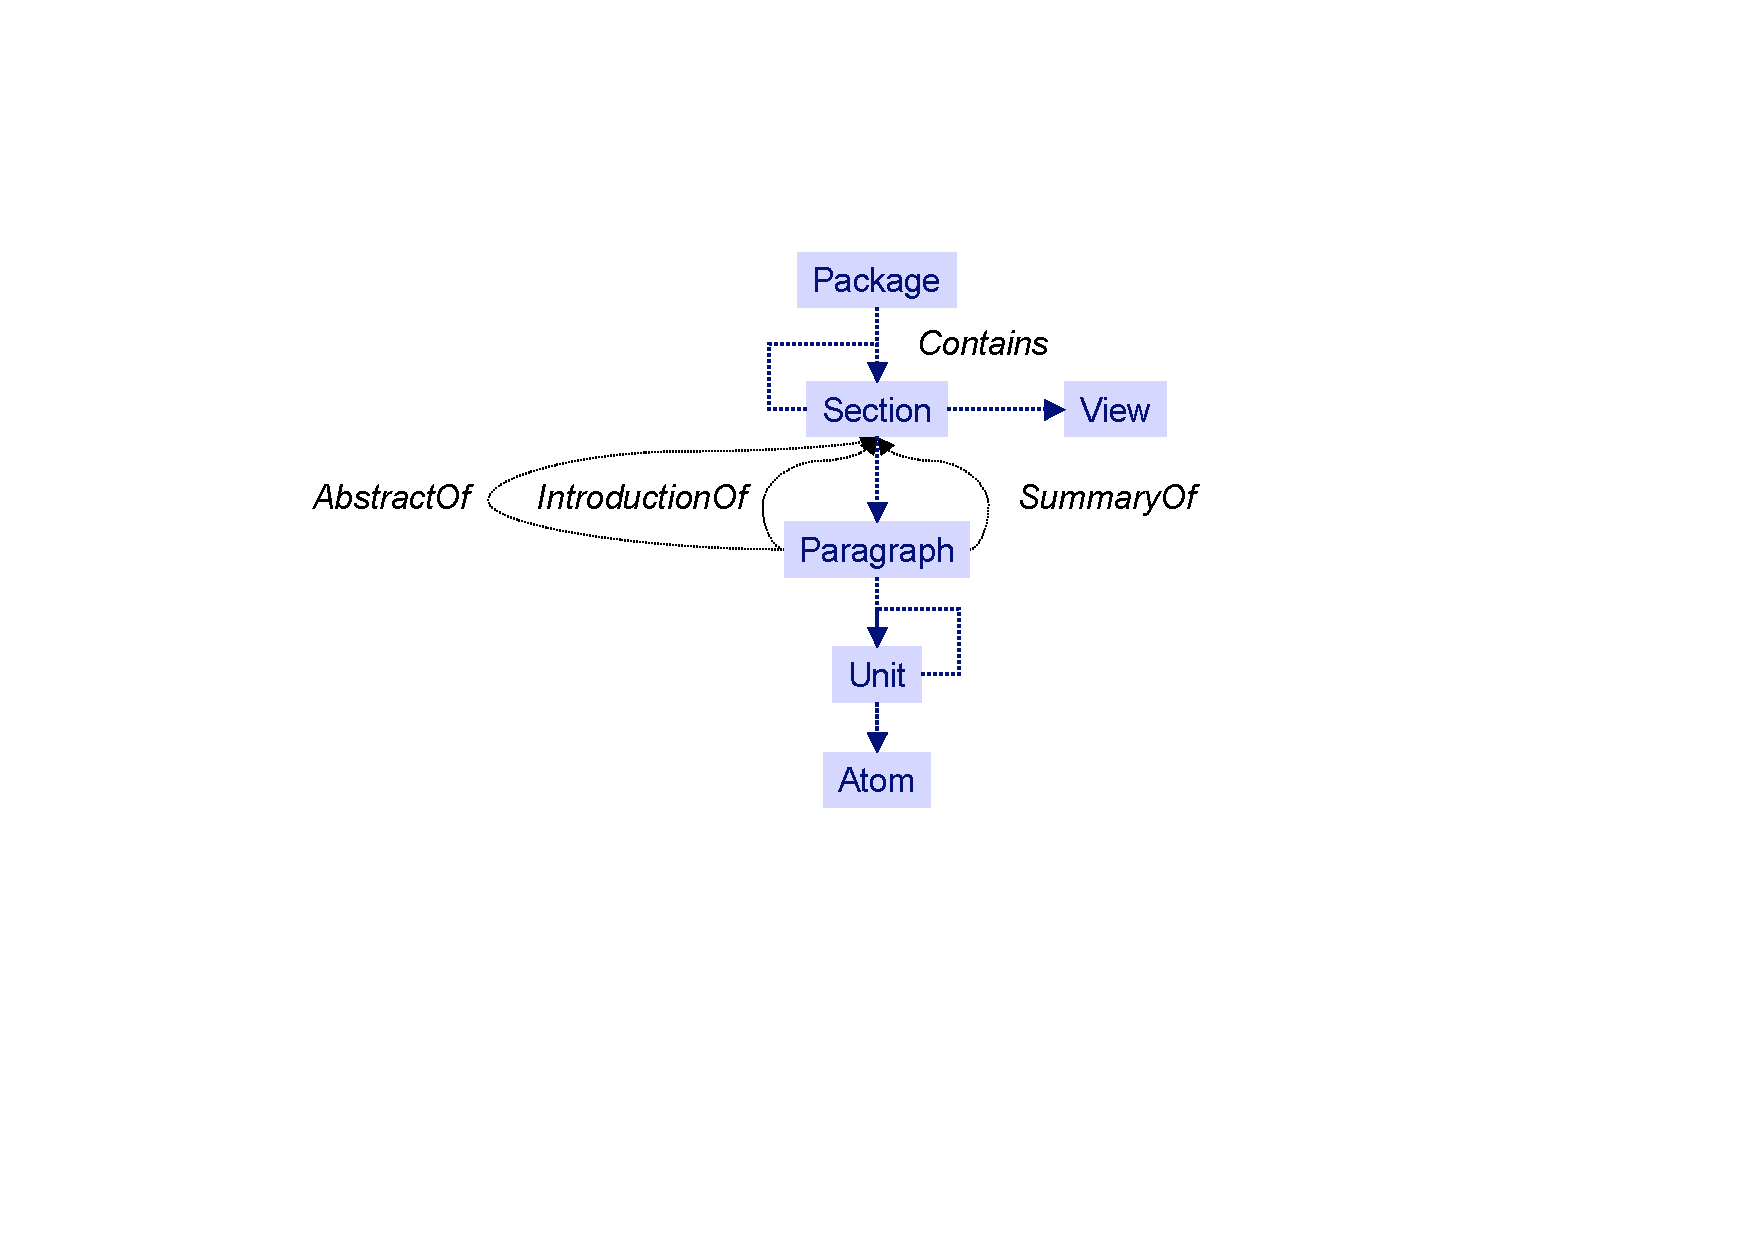
\includegraphics[width=\textwidth]{img/document-structure-ontology}
    \caption{Document Structure Ontology.}
    \label{fig:document-structure-ontology}
  \end{center}
\end{figure}

\begin{figure}[htbp]
  \begin{center}
    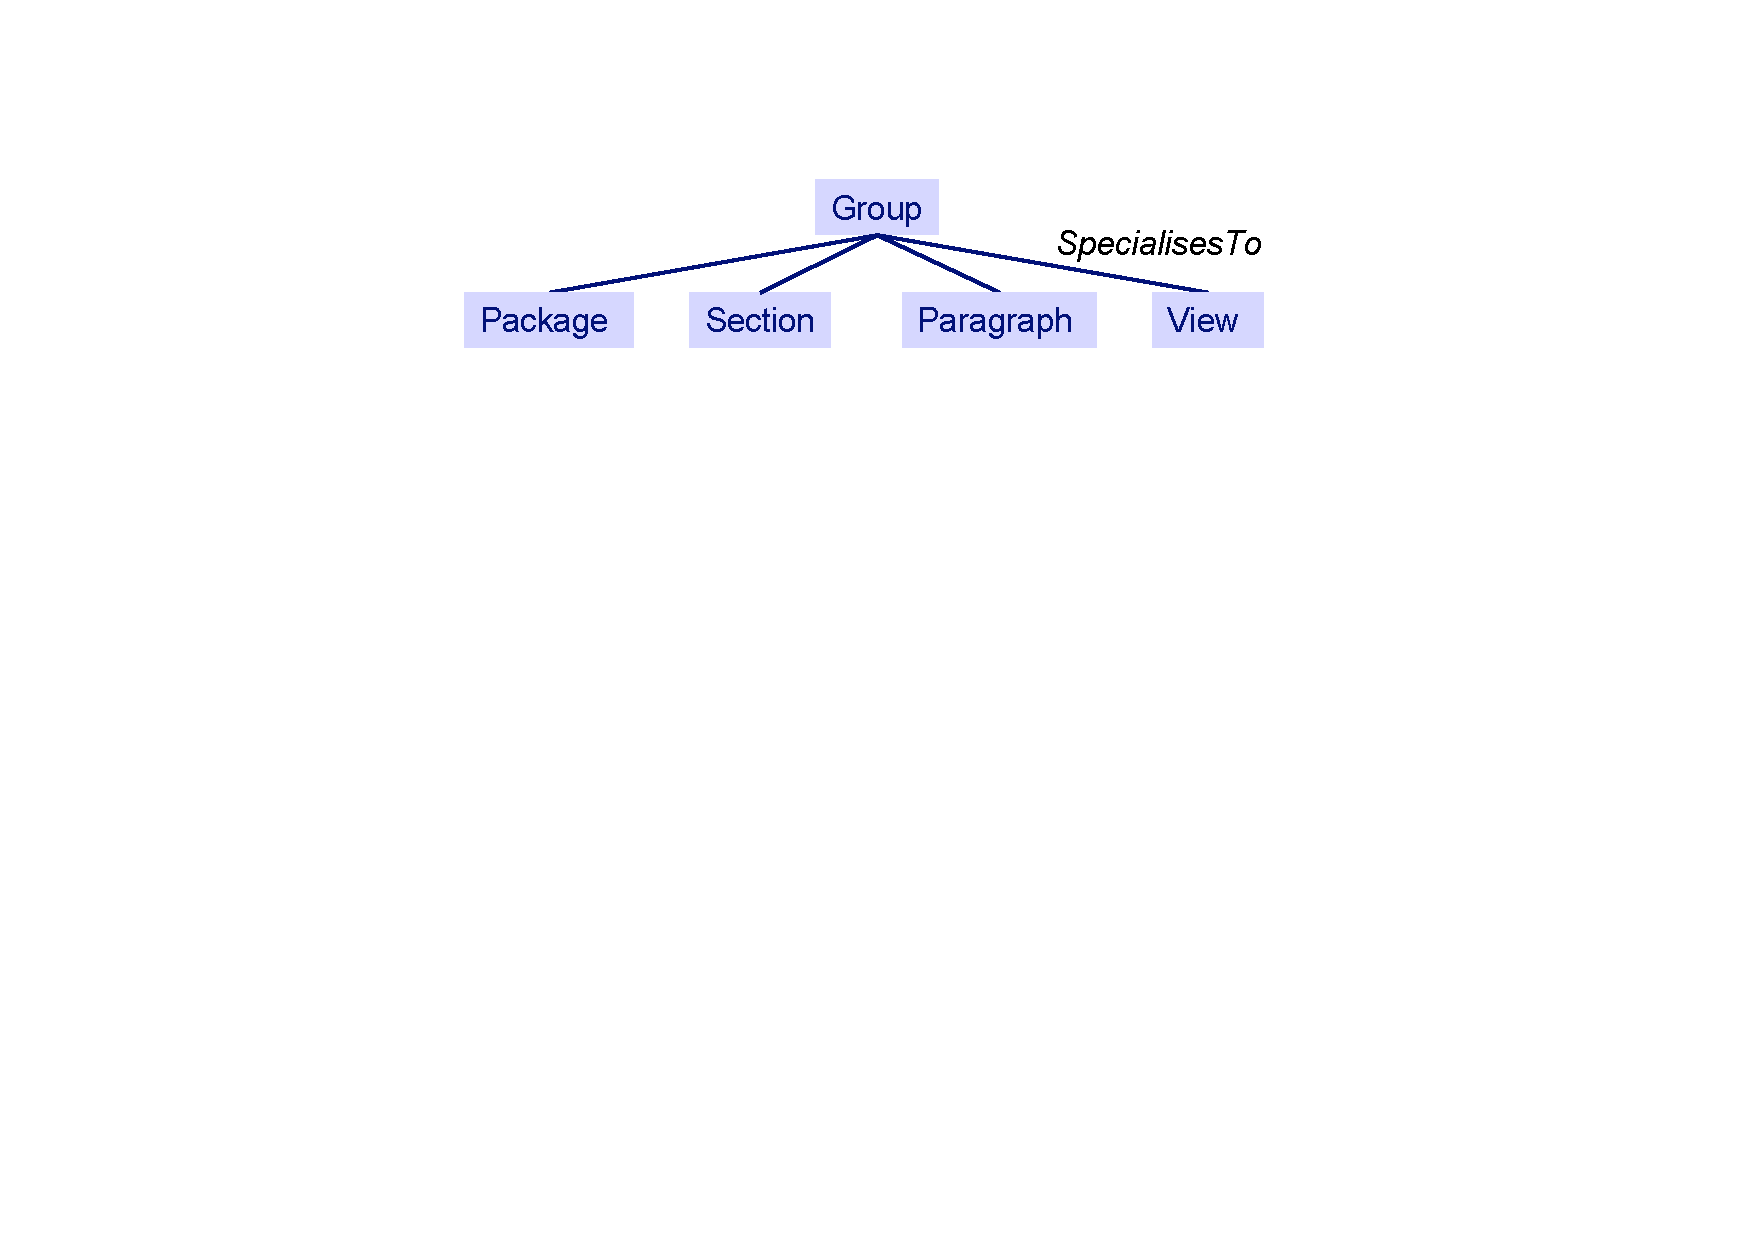
\includegraphics[width=\textwidth]{img/Groups-ontology}
    \caption{Ontology for Groups.}
    \label{fig:Groups-ontology}
  \end{center}
\end{figure}


\begin{figure}[htbp]
  \begin{center}
    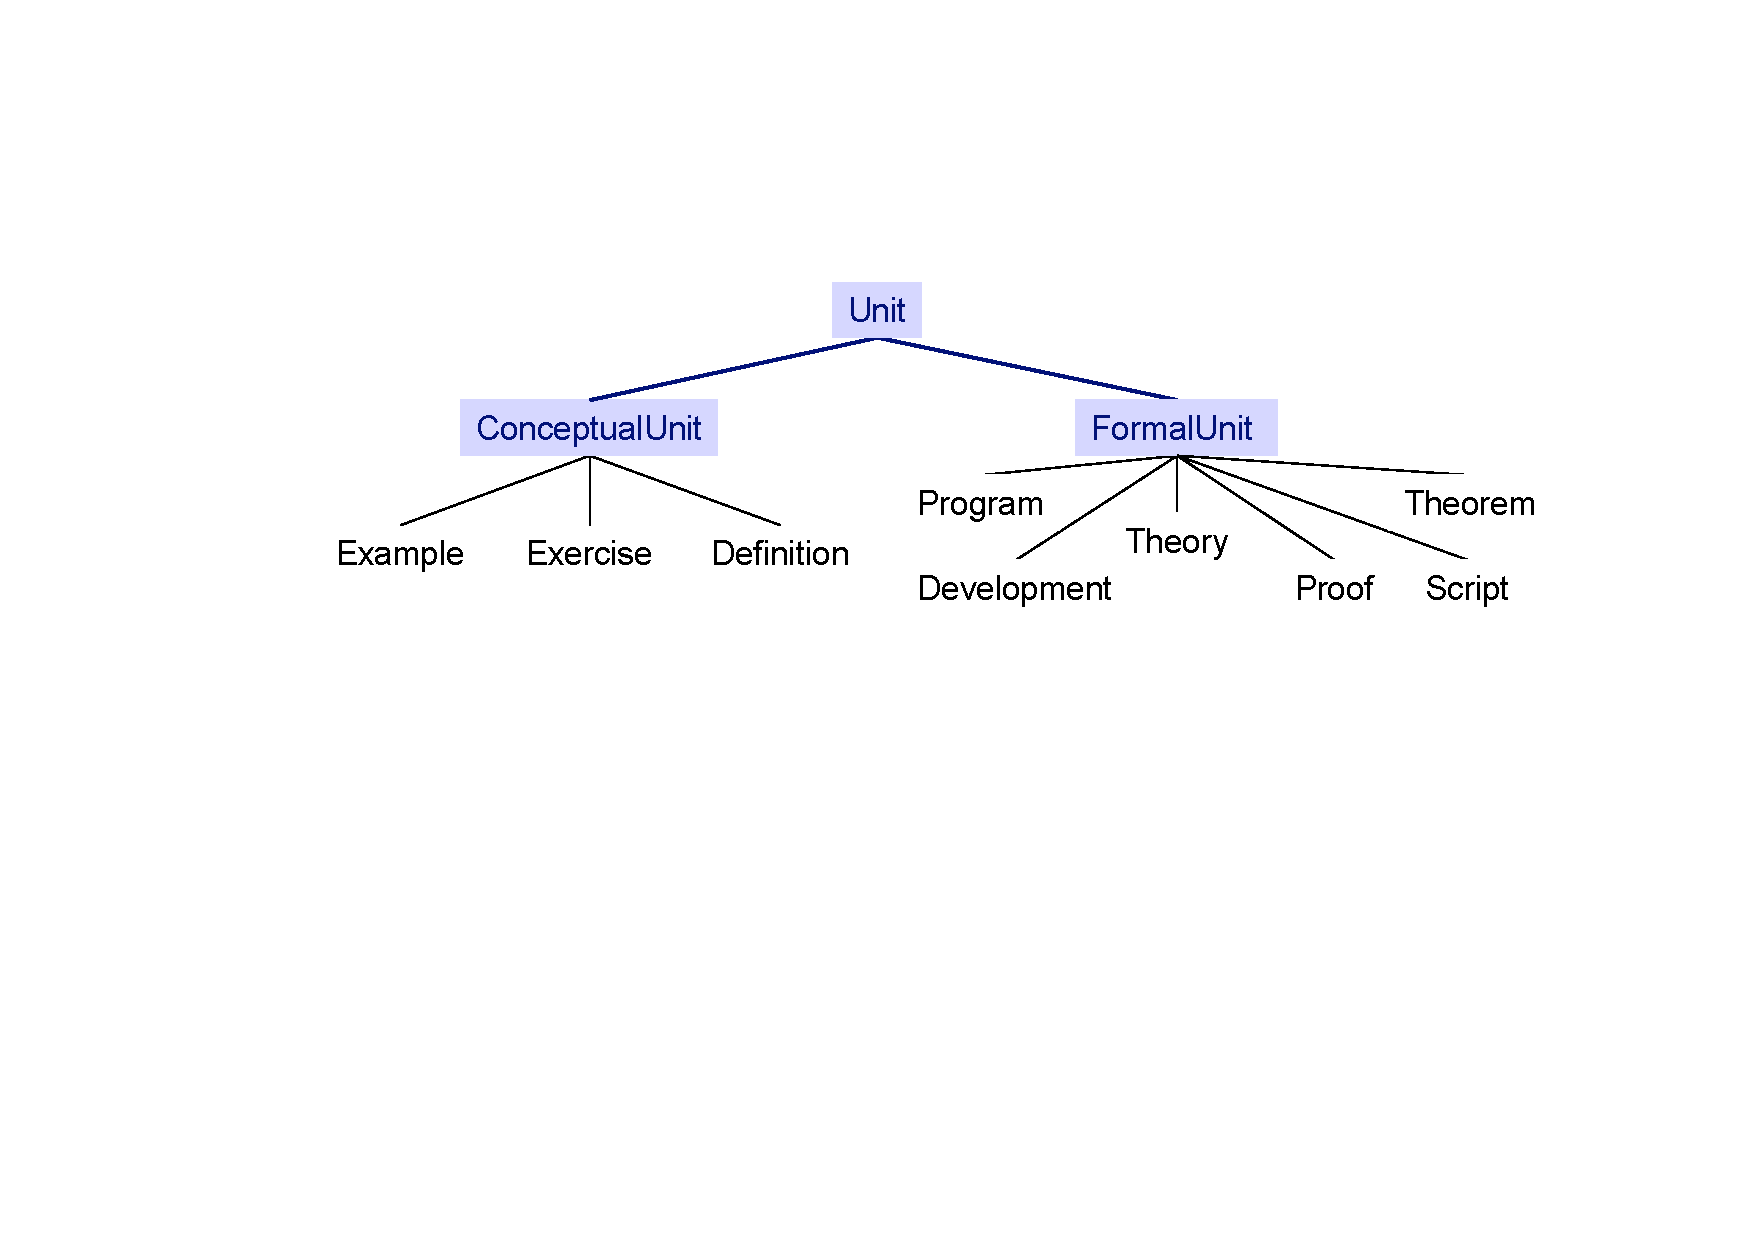
\includegraphics[width=\textwidth]{img/Units2-ontology}
    \caption{Ontology for Units.}
    \label{fig:Units-ontology}
  \end{center}
\end{figure}

\begin{figure}[htbp]
  \begin{center}
    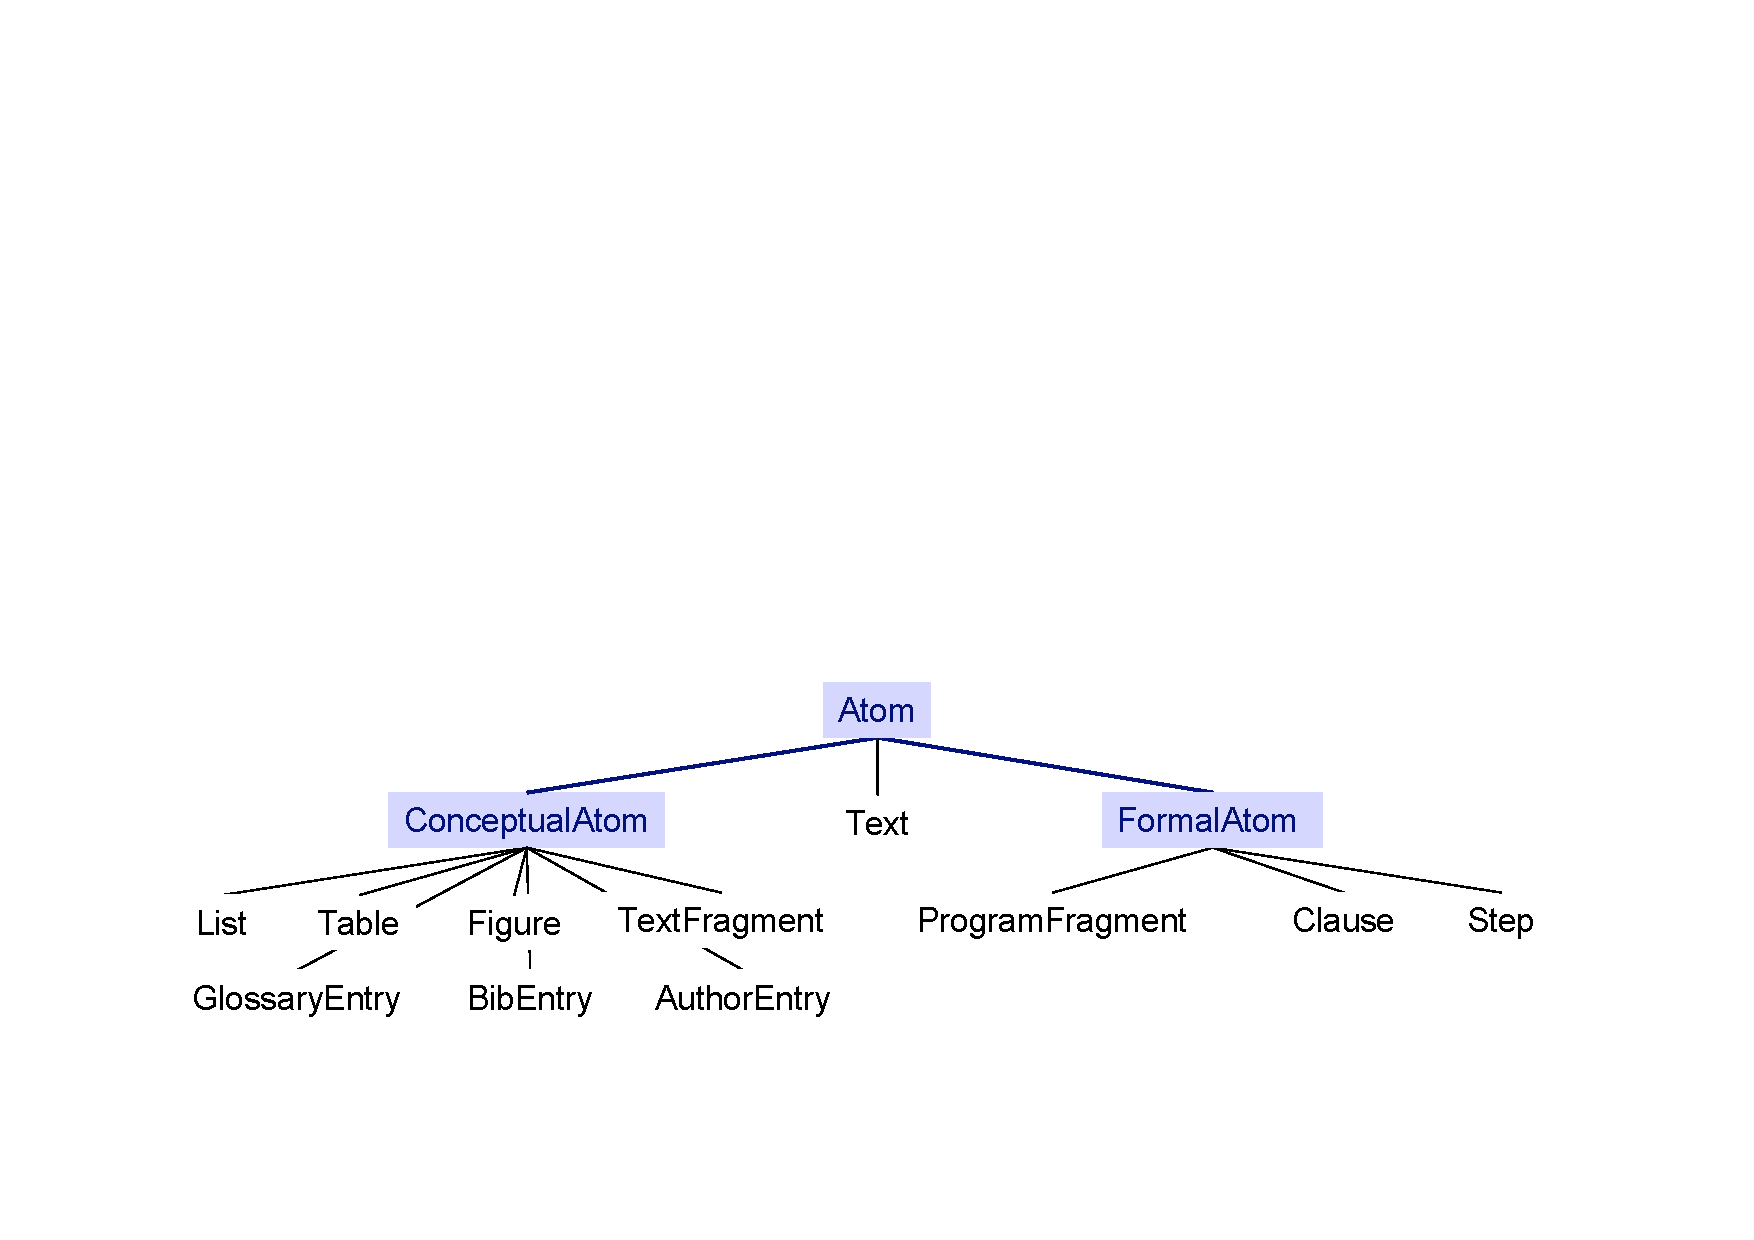
\includegraphics[width=\textwidth]{img/Atoms3-ontology}
    \caption{Ontology for Atoms.}
    \label{fig:Atoms-ontology}
  \end{center}
\end{figure}


\paragraph{Structural Entities}
The primary purpose of structuring documents is conceptual. We are used to textually nest paragraphs 
\MarginComment{JGS ``We are used to nest'' ist kein korrektes
  Englisch. ``We use to nest'' oder besser ``we are used to nesting''}
in sections, and sections in other sections, possibly classified into (sub)subsections, chapters, parts of
documents or the like. The same is true here, cf. Fig.~\ref{fig:document-structure-ontology} that shows part
of the ontology of \MMiSS{} 
\MarginComment{JGS: Diese geh{\"a}uften Doppelpunkte sind irgendwie seltsam.}
\DefClass{DocStructuringOperation}{\DocStructuringOperation}s: 
yielding particular kinds of
\DefClass{StructuralEntities}{\StructuralEntities}: 
\DefClass{SectionStr}{\SectionStr}s
may be nested; they
are not classified as chapters or the like to ease re-structuring without the need for renaming operators
(section numbering etc. is, if desired, done automatically anyway during layout). 
As we see in Fig.~\ref{fig:document-structure-ontology} and 
Fig.~\ref{fig:Groups-ontology}, the
largest of the 
\DefClass{GroupStr}{\GroupStr}
\StructuralEntities{} for
structuring in-the-large is a 
\DefClass{PackageStr}{\PackageStr};
\PackageStr{}s may be semantically related, see
Sect.~\ref{sec:packages}. 
A 
\DefClass{ParagraphStr}{\ParagraphStr}
 is the smallest 
of the \StructuralEntities{}, whose title might appear in a table of contents 
--- it should correspond to a single
slide in a lecture, or possibly one plus a continuation slide with the same title. 

Each \SectionStr{}
should contain three special  sub-\SectionStr{}s or \ParagraphStr{}s: The
\DefClass{AbstractStr}{\AbstractStr}
contains an overview of the \SectionStr{}; the 
\DefClass{IntroductionStr}{\IntroductionStr}
gives a motivation for the content to come and sets a didactic goal (``what we are about to learn''); the 
\DefClass{SummaryStr}{\SummaryStr}
at the end recalls the highlights of the content (``what we have learned''). Note that there are no explicit ``transition'' \ParagraphStr{}s between \SectionStr{}s since they would assume a given {\Order} (see the Sec.~\ref{sec:order}); instead, the \IntroductionStr{} should refer to the upper context (``what we already know''), if necessary, and the \SummaryStr{} should provide forward references to the lower context (``what we will learn more about'') in subsequent \SectionStr{}s.

A {\ParagraphStr} may contain 
\DefClass{UnitStr}{\UnitStr}s
and {\UnitStr}s may contain other 
{\UnitStr}s or 
\DefClass{AtomStr}{\AtomStr}s.
A {\UnitStr} is an entity one would like to be able to keep together and eventually present as 
a whole as far as possible, i.e. on one slide in a lecture or on one page in a book.
The \UnitStr{} is the primary structuring facility, classifying the enclosed content to be of a particular kind, e.g. a {\TheoryStr} in a particular {\FormalismAttribute} such as \CASL{}; it is the major unit of change (corresponding to a node in the {\StructureGraph},
%Development Graph, 
see {\ChangeManagement} in 
Sect.~\ref{sec:change-management}) and the minimal context for editing. 

As we see in Fig.~\ref{fig:Units-ontology},
{\UnitStr}s of a particular kind, e.g. 
\DefClass{DefinitionStr}{\DefinitionStr}s,
\DefClass{ExampleStr}{\ExampleStr}s, or
\DefClass{ExerciseStr}{\ExerciseStr}s,
can be specially identified in a 
document and e.g. collected into a list of exercises in an appendix (cf. views in
Sect.~\ref{sec:views}).


As we see in Fig.~\ref{fig:document-structure-ontology} and Fig.~\ref{fig:Atoms-ontology},
an {\AtomStr} such as 
\DefClass{TextStr}{\TextStr},
a labelled 
\DefClass{TextFragmentStr}{\TextFragmentStr}, a
\DefClass{FigureStr}{\FigureStr} or a
\DefClass{TableStr}{\TableStr},
is an indivisible leaf of structuring
and the smallest of the \StructuralEntities{} that can be shared (see Sec.~\ref{sec:sharing} on {\StructuralSharing}); it is usually not shown in the {\StructureGraph}
%Development Graph 
unless a visualisation of the micro-structure of a \UnitStr{} is explicitly requested. 
\end{Paragraph}
\end{Section}

\begin{Section}[Title={Conceptual and Formal Structure},Label={Conceptual_and_Formal_Structure}]
\begin{Paragraph}
%\subsubsection{Conceptual and Formal Structure}


\MarginComment{JGS: Findet Ihr das gut, dass wir Seiten nur mit
  Abbildungen haben, die noch nicht einmal voll sind?}

        \begin{figure}[htbp]
          \begin{center}
            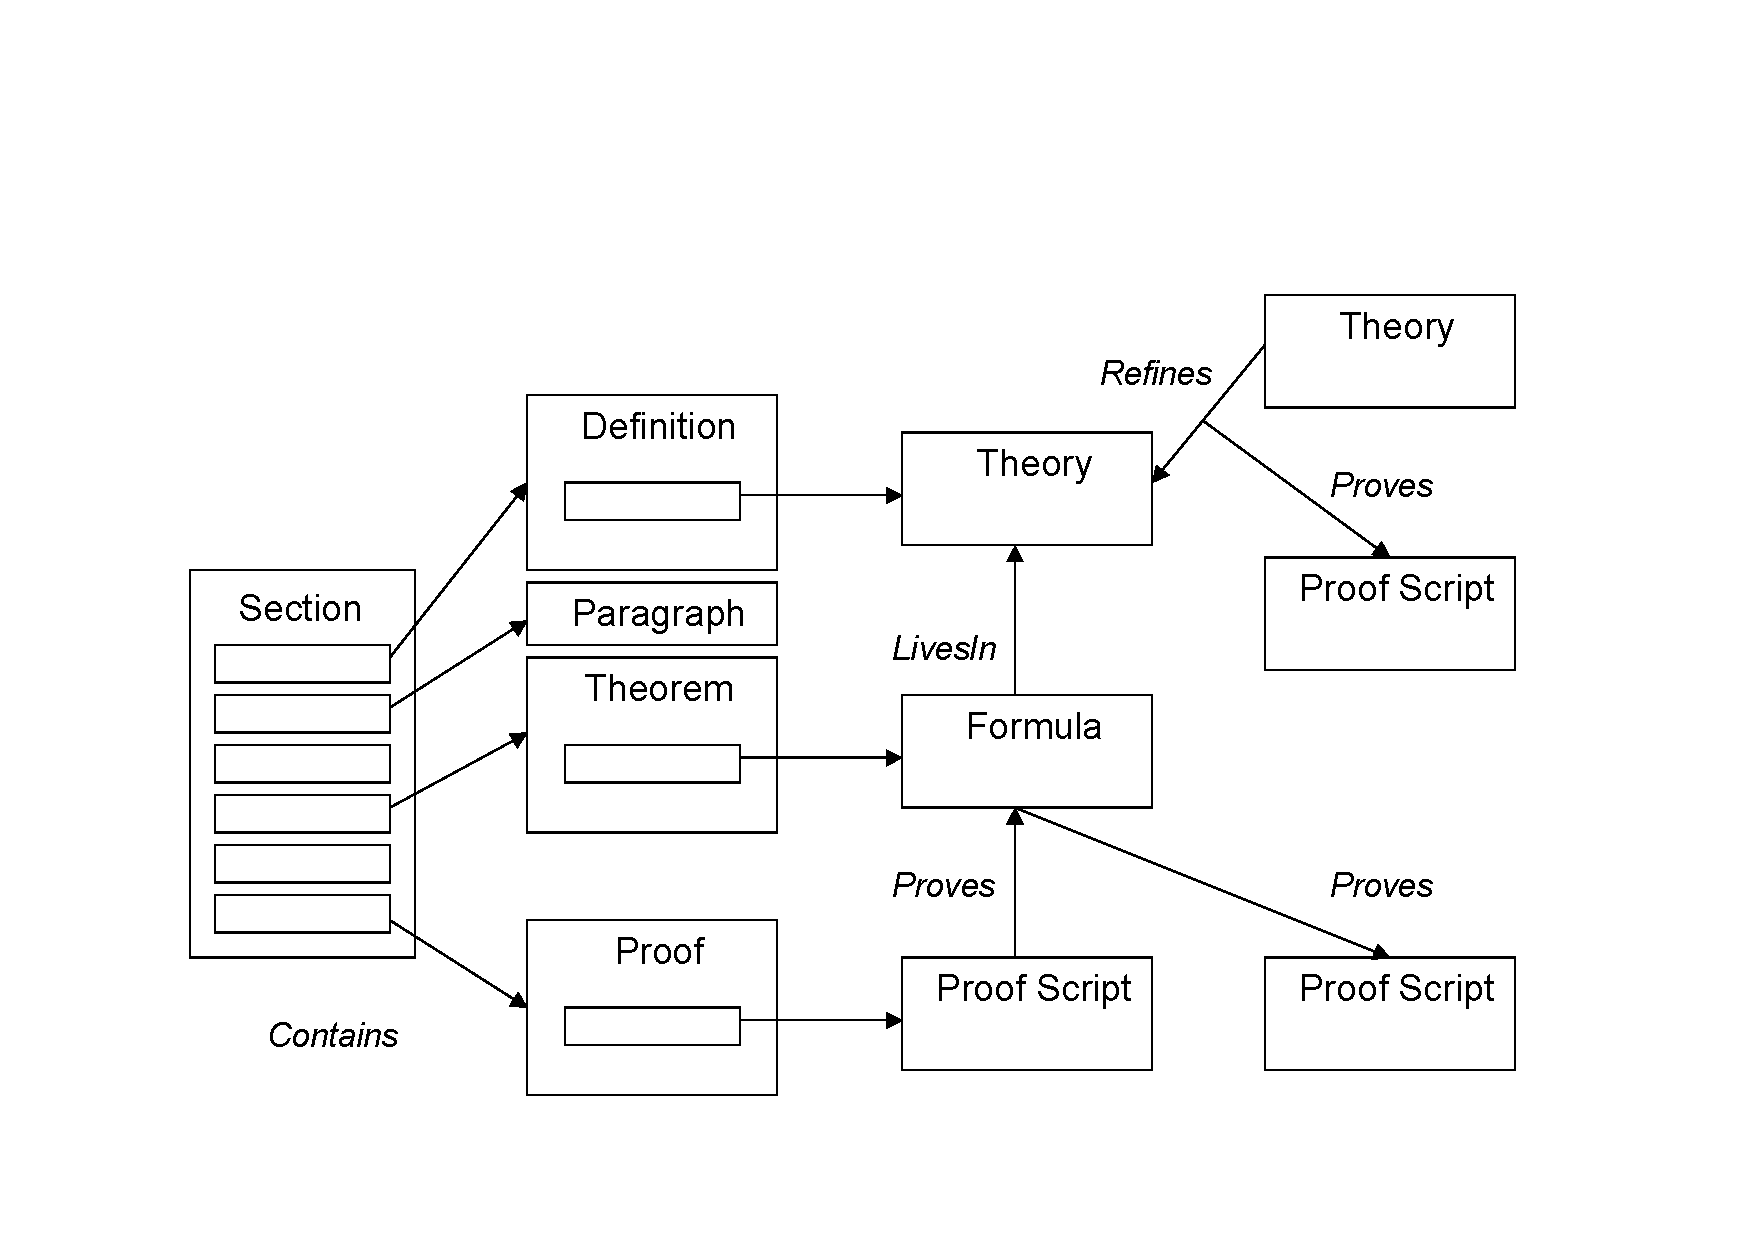
\includegraphics[width=\textwidth]{img/ExConfigurations1}
            \caption{Conceptual and Formal Structure.}
            \label{fig:conceptual-and-formal-structure}
          \end{center}
        \end{figure}

The document structure ontology in Fig.~\ref{fig:document-structure-ontology}, Fig.~\ref{fig:Groups-ontology}, Fig.~\ref{fig:Units-ontology}, and Fig.~\ref{fig:Atoms-ontology} is tailored to
the  particular application domain of the \MMiSS{} project: safe and secure systems with formal methods.
While it is meant to be generally applicable and extensible, it also specially caters for formal, e.g.
mathematical, documents.  Therefore some of the {\UnitStr}s are classified as
\DefClass{FormalUnitStr}{\FormalUnitStr}s,
similarly for 
\DefClass{FormalAtomStr}{\FormalAtomStr}s;
these are associated with a particular 
\DefClass{FormalismAttribute}{\FormalismAttribute}.
A {\FormalismAttribute} has, in general, a formal syntax and (hopefully more often than not) a 
formal semantics. Examples are a 
\DefClass{ProgramStr}{\ProgramStr}
in a programming language or a
\DefClass{TheoryStr}{\TheoryStr}
in a specification language.  Thus a 
\FormalAtomStr{}
such as an 
\DefClass{AxiomStr}{\AxiomStr},
while being atomic
from a document structuring point of view,  may indeed have further substructure when analysed by a
specialised tool.

This way the \StructuralEntities{}  of the conceptual structure contain those of the formal structure
(cf. Fig.~\ref{fig:ExConfigurations1}). 
A particular document may contain consistent formal sub-documents, e.g. complete executable \ProgramStr{}s or
complete theories (cf. also views in Sect.~\ref{sec:views}) that can be analysed together.

\MarginComment{JGS: Der Befehl
\texttt{$\backslash$paragraph} wir nur dreimal benutzt und es sieht wie ein
Fehler aus, da die {\"U}berschrift anders gesetzt ist als f{\"u}r 
\texttt{$\backslash$subsubsection}. Man denkt, es m{\"u}sste eigentlich das Gleiche
sein. Au{\ss}erdem ist die {\"U}berschrift direkt am Zeilenanfang oft
irritierend, wenn sie nicht von einem Punkt gefolgt wird.} 
\end{Paragraph}
\end{Section}

\begin{Section}[Title={Sharing},Label=Sharing]
\begin{Paragraph}
%\subsubsection{Sharing}
\label{sec:sharing}

        \begin{figure}[htbp]
          \begin{center}
            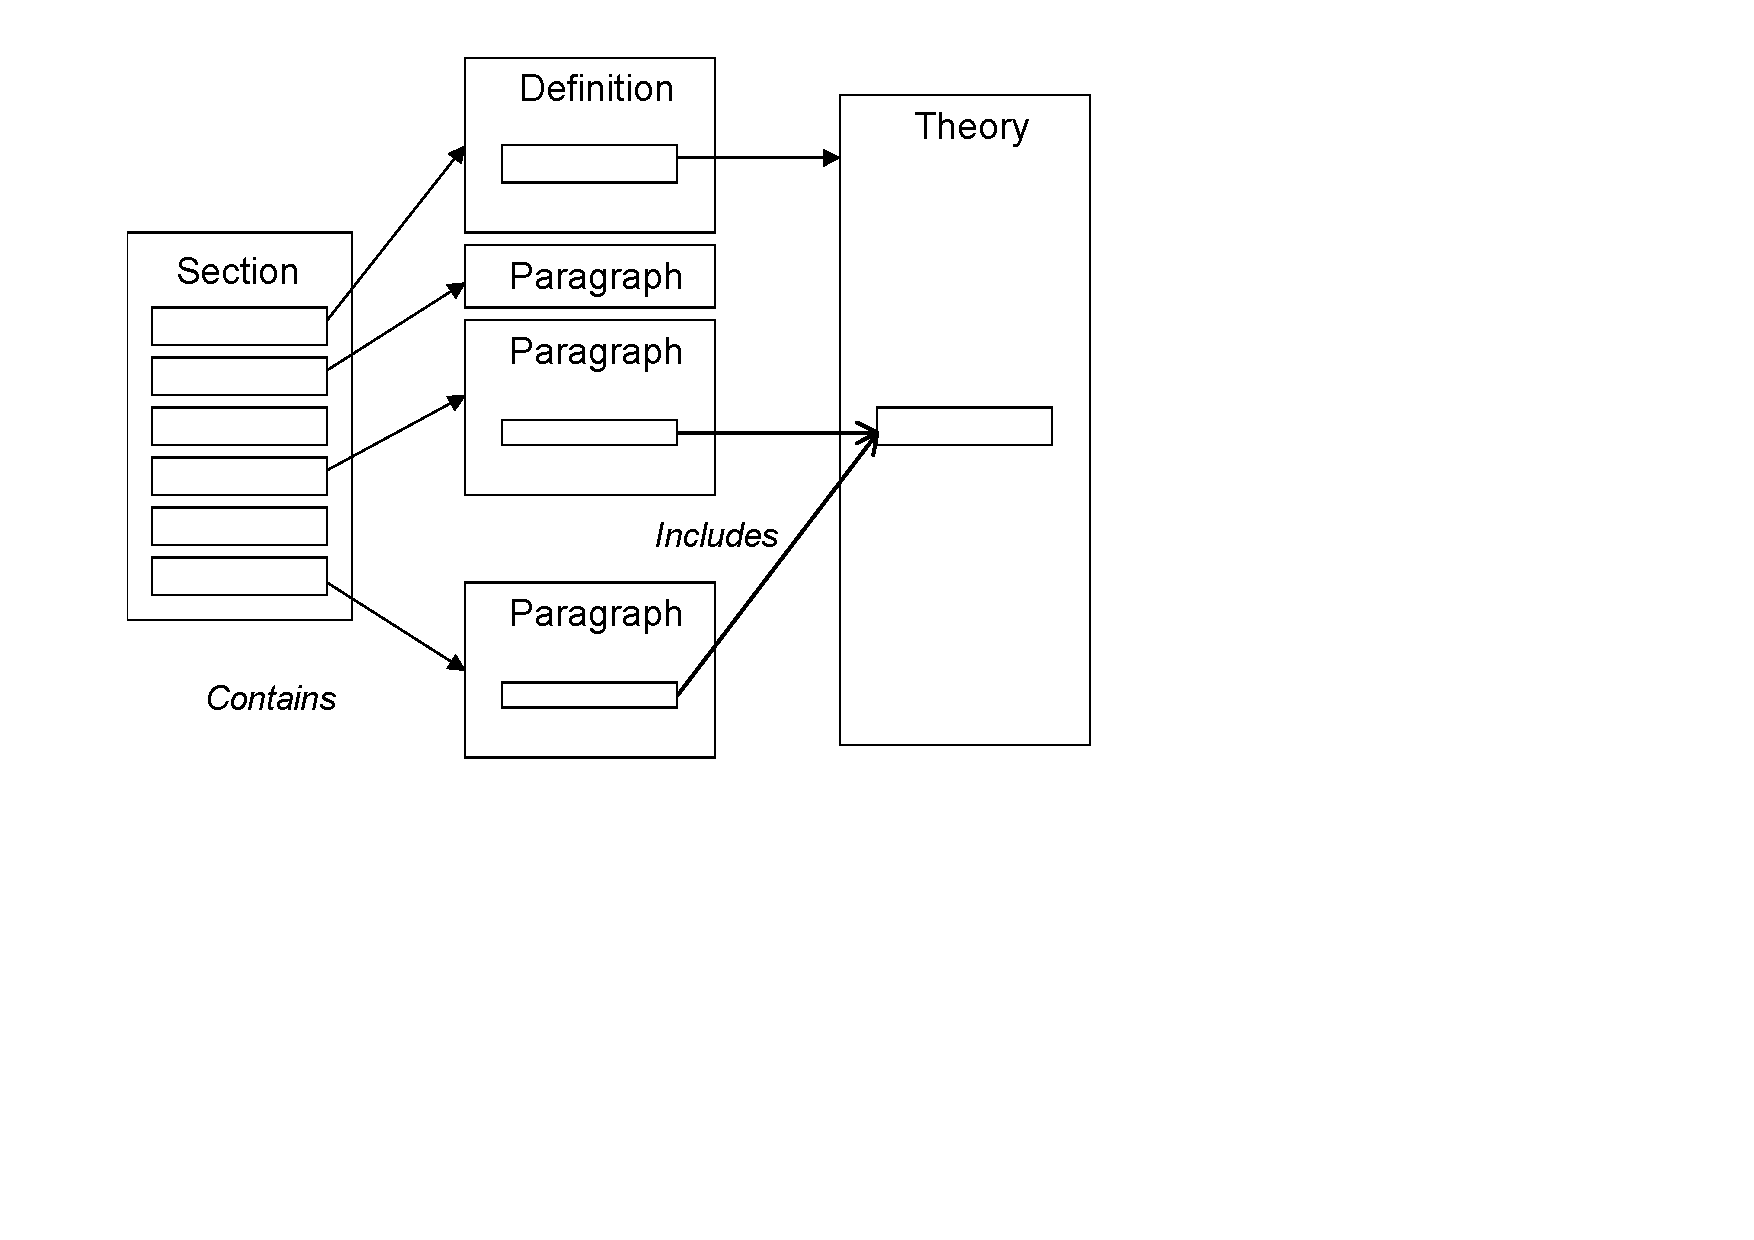
\includegraphics[width=\textwidth]{img/ExSharing2}
            \caption{Sharing.}
            \label{fig:sharing}
          \end{center}
        \end{figure}

Formal entities may be embedded piecewise (e.g. an {\AxiomStr} of a {\TheoryStr}), 
as they are being introduced and explained from a conceptual or pedagogical point of view. 
However, it is also a good idea to present them together, possibly in a separate part of the same 
document (e.g. an appendix), to exhibit a consistent whole, both from a conceptual point of view (e.g. a
complete {\TheoryStr} with all fragments put together) and the technical consideration of having a
complete formal document that can be treated by a tool (e.g. analysis of a complete {\TheoryStr} or
execution of a {\ProgramStr} with input data). Note also that it is often necessary for pedagogical
purposes to be able to present alternatives and variations in a document, even incomplete or intentionally
wrong ones that should not be subjected to formal analysis. 

An entity should appear in more than one place, e.g. as an {\AxiomStr} in an 
explanatory \ParagraphStr{} and as part of a consistent and complete {\TheoryStr} in an appendix
(cf. Fig.~\ref{fig:sharing}).  A copy
will not do; common experience dictates that two copies of the ``same'' entity have a tendency to differ
eventually. Thus  
\DefClass{StructuralSharing}{\StructuralSharing}
is needed, avoiding the danger of un-intentional difference: an
{\AxiomStr} named by a {\LabelAttribute}
in one part of a document (or a different document)
may be included, with a link to this \LabelAttribute{}, in another.  It is technically immaterial,
whether the {\AxiomStr} appears in the {\ParagraphStr}  and the include operation in the
{\TheoryStr}, or vice versa. This operation will trigger a textual expansion in the presentation of the
document such that both occurrences are indistinguishable in the presentation. In the source, the
{\AxiomStr} has a ``home'' where it can be edited, whereas it cannot be edited at the positions of
the include operation (it appears ``frozen'' in a wysiwyg-editor). From a methodological point of view, it is
preferable to maintain a complete {\TheoryStr},  which is, however, structured in such a way that
links to a particular {\AxiomStr} are possible from other places.
\BKB{more about Knuth's literate programming}

Sharing is not restricted to formal entities. Indeed, whole sub-documents can be shared when 
composing a new document from bits and pieces of existing ones, 
cf. views in Sect.~\ref{sec:views}.

\subsubsection{Structural Links}

Apart from the implicit links of include operations, classical (hyper-)links to \StructuralEntities{} are
\MarginComment{JGS: ``available called'' $\to$ ``available and called''?}
available called
\DefClass{LinkStr}{\LinkStr}s. 
We will see in Sect.~\ref{sec:variants} that these may be subject to variant selection, possibly
with multiple links.

The textual nesting and the include operations give rise to 
\DefRelation{Contains}{\Contains} relations 
corresponding to 
arrows in a directed acyclic \Graph{}, the {\StructureGraph}, see
Sect.~\ref{sec:variants} and Sect.~\ref{sec:structure-graph}.
\end{Paragraph}
\end{Section}
\end{Section}

\begin{Section}[Title={Attributes},Label={Attributes}]
\begin{Paragraph}
%\subsection{Attributes}
\label{sec:attributes}

\begin{figure}[htbp]
  \begin{center}
    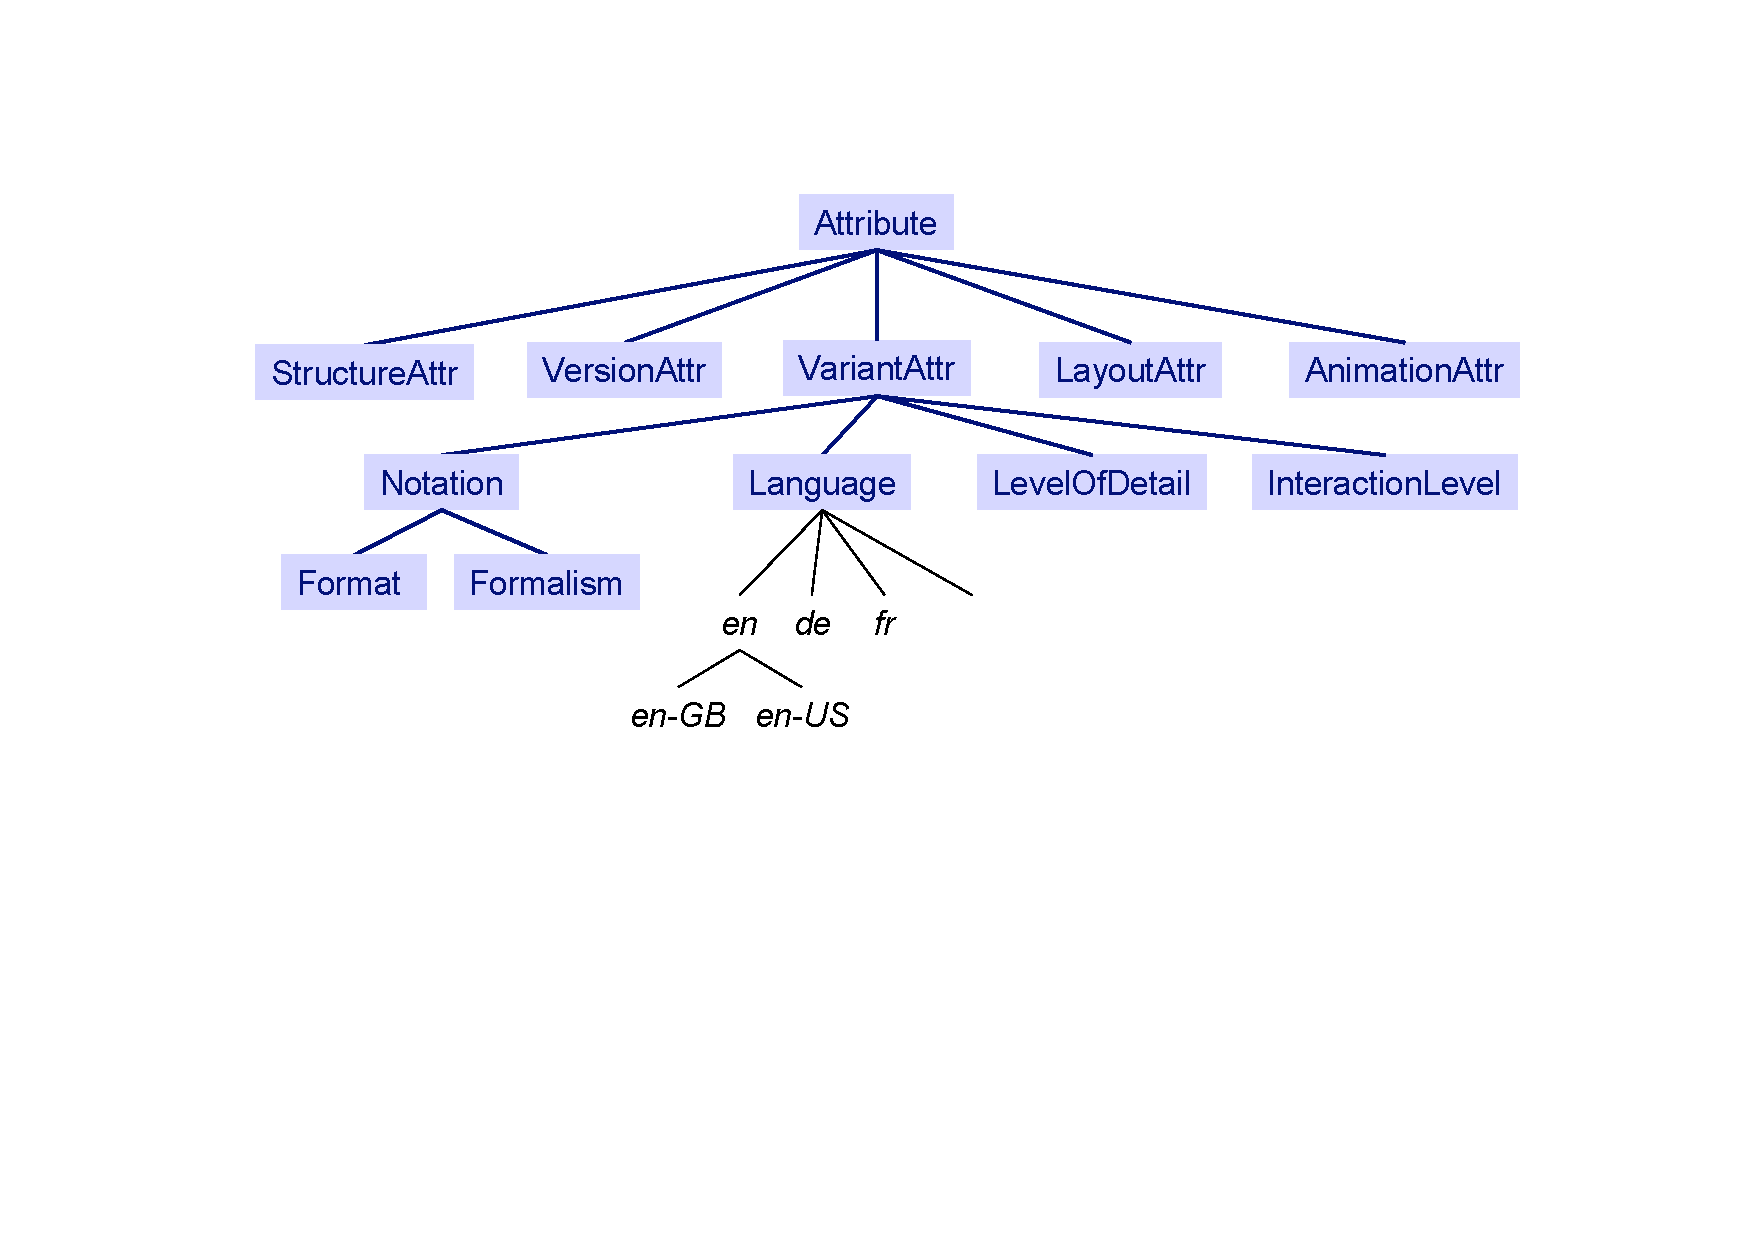
\includegraphics[width=\textwidth]{img/attribute-ontology}
    \caption{(Partial) Attribute Ontology}
    \label{fig:attribute-ontology}
  \end{center}
\end{figure}


The possibility to define 
\DefClass{Attribute}{\Attribute}s
is a central feature for \StructuralEntities{}, cf. Fig.~\ref{fig:attribute-ontology}. 
Standard 
\DefClass{StructureAttribute}{\StructureAttribute}s
are e.g. the individual
\DefObject{LabelAttribute}{\LabelAttribute}
and  
\DefObject{TitleAttribute}{\TitleAttribute}
of some \SectionStr{} or \ParagraphStr{}.

\subsubsection{Inheritance of Attributes}
Most importantly, 
\DefClass{AttributeInheritance}{\AttributeInheritance}
to nested \StructuralEntities{} relieves the author from specifying {\Attribute}s over and over again and
avoids cluttering; at the same time, an {\Attribute} may be superseded for a nested ``subtree'' of
\StructuralEntities{}.
\end{Paragraph}

\begin{Section}[Title={Author and Version Attributes},Label={Author_and_Version_Attributes}]
\begin{Paragraph}
%\subsubsection{Author and Version Attributes}
Each of the \StructuralEntities{} has an
\DefObject{AuthorsAttribute}{\AuthorsAttribute}
and a
\DefClass{VersionAttribute}{\VersionAttribute}
(see also {\VersionControl} in Sect.~\ref{sec:version-control}).
These \Attribute{}s record the author(s) of each fragment (inherited to nested \StructuralEntities{}) 
and keep track of \PriorAuthorsAttribute{} and the authorship of individual \Revision{}s.
\end{Paragraph}
\end{Section}

\begin{Section}[Title={Layout and Animation Attributes},Label={Layout_and_Animation_Attributes}]
\begin{Paragraph}
%\subsubsection{Layout and Animation Attributes}
\label{sec:layout-attributes}
As will be discussed further in Sect.~\ref{Layout-MMiSSLaTeX} and \ref{Animation-MMiSSLaTeX}, \Presentation{} issues such as 
\Layout{} and \Animation{} should be separable from the ``logical'' content of \StructuralEntities{} and should be confined to the necessary only. 
It is a relief that these can be specified independently as attributes and that \AttributeInheritance{} takes 
care of otherwise tedious repetition of logically irrelevant presentation detail. 
The specification, for example, that list items on a slide should be rolled out one after another could be 
specified a the root of a (sub)document and applies to it as a whole unless re-specified for a nested subdocument.
Similarly, a revision of such a specification need only be made at the root.
\end{Paragraph}
\end{Section}
\end{Section}

\begin{Section}[Title={Variants},Label={Variants}]
\begin{Paragraph}
%\subsection{Variants}
\label{sec:variants}


Perhaps the most innovative feature of the \MMiSS{} project is the definition of
\DefClass{VariantAttribute}{\VariantAttribute}s
and the management of documents with several different
\DefClass{Variant}{\Variant}s
in a consistent way.
\end{Paragraph}

\begin{Section}[Title={Natural Languages},Label={Natural_Languages}]
\begin{Paragraph}
%\subsubsection{Natural Languages}

Let us take the 
\DefClass{LanguageAttribute}{\LanguageAttribute} attribute
as an example, cf. Fig.~\ref{fig:attribute-ontology}. 
A Language attribute specifies the natural language in which a text is written, following the language codes of IETF RFC 1766 / ISO 639. The default is 
\DefObject{enGBAttribute}{\enGBAttribute}
(British English), overriding the standard
\DefObject{AnyAttribute}{\AnyAttribute} attribute
that is usually the default for the other \VariantAttribute{}s. 
Another example is
\DefObject{deAttribute}{\deAttribute}
(German).

Let us now assume that an author wants to manage e.g. English and German documents in parallel. Most probably, the author would want the structure of the two documents to be identical as they are being used for the same purpose, e.g. slides for a 
{\LectureAttribute}. 
In this case, s/he may edit two copies of the same document side by side, e.g. in two separate windows of the \XEmacsEditor{} (cf. Sec.~\ref{sec:user-interfaces}). 
These two {\Version}s should have the same structure, i.e. the same \StructuralEntities{}, nested in the same way, where each of them has the same \LabelAttribute{} as in the other {\Version}, resp. This ensures that the structures of the two {\Version}s can be compared, and are consistent and complete, during 
{\ConfigurationManagement} 
(cf. Sec.~\ref{sec:version-control}). In fact, in the {\Repository} the two {\Version}s of the document are merged such that two {\Version}s can be identified for each of the \StructuralEntities{}. 
Thus the author may also edit one {\Version} first and then the other step by step, for each of the \StructuralEntities{} separately, along the structure of the first. Similarly, an individual {\Revision} for one of the  \StructuralEntities{} is possible, with the two {\Version}s side by side.

\BKB{to be edited}
\MarginComment{JGS:\\ ``manage-ment''?}
A structural element that appears in several variants retains the same Id; configuration manage-ment will ensure compatible variants for a particular configuration in a View. If no VariantAttr in a particular variant domain (e.g. no LevelOfDetailId) is inherited or given explicitly, the special attribute value ANY is assumed by default, i.e. the respective structural element is meant to be acceptable for any value in this domain (e.g. any level of detail). To stop implicit inheritance, this value may be given explicitly.
\end{Paragraph}
\end{Section}

\begin{Section}[Title={Notations, Formats and Formalisms},Label=s16]
\begin{Paragraph}
%\subsubsection{Notations, Formats and Formalisms}

\begin{figure}[htbp]
  \begin{center}
    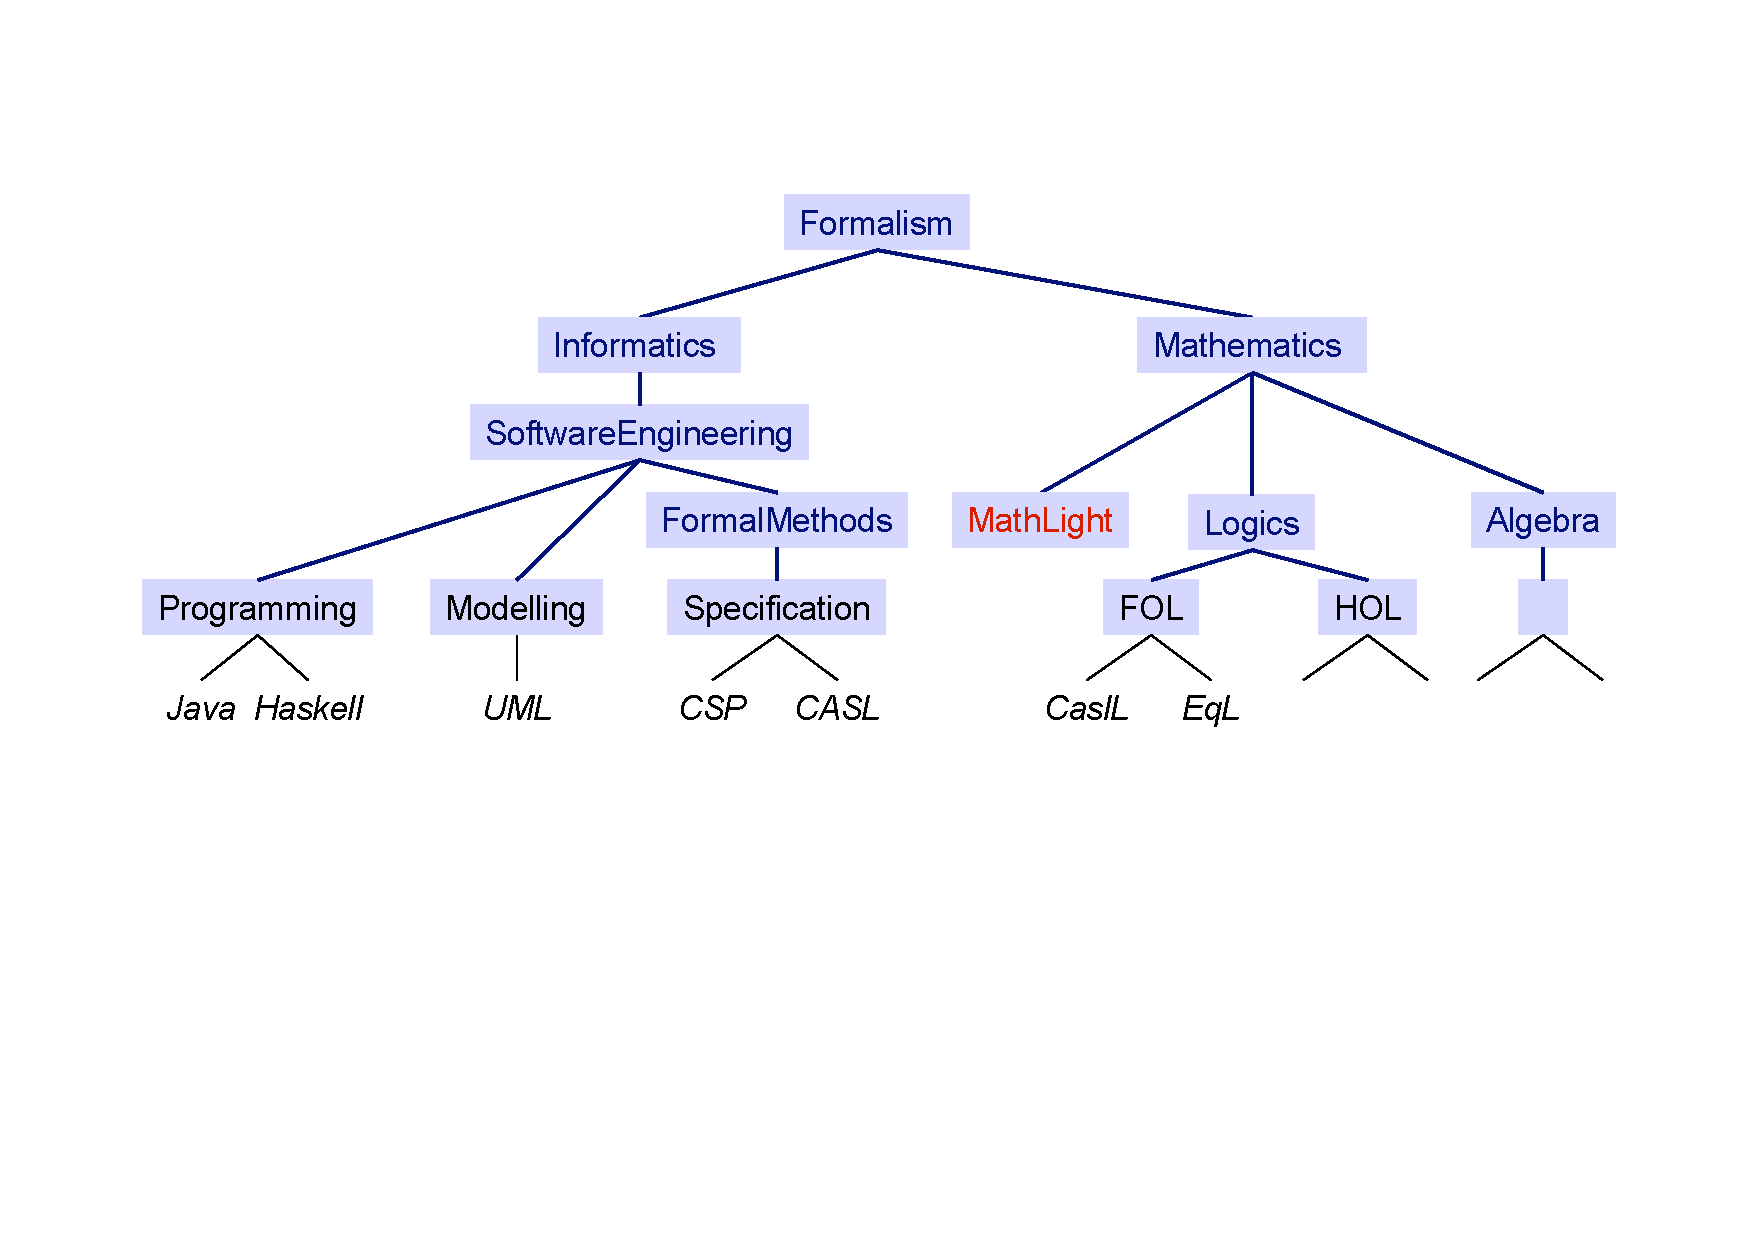
\includegraphics[width=\textwidth]{img/formalisms-ontology}
    \caption{(Partial) Ontology of Formalisms.}
    \label{fig:formalisms-ontology}
  \end{center}
\end{figure}

\DefClass{NotationAttribute}{\NotationAttribute}
embed mathematical formulae, programs, etc. 
LaTEX formulae, tool interface

\BKB{to be edited}
%Conceptual \UnitStr{}s or \AtomStr{}s are standard for all subject domains. A \FormalUnitStr{} or \AtomStr{} is usually expressed in a particular \FormalismAttribute{} that is well-defined, i.e. it has a special syntax and (formal) semantics. The substructure of \AtomStr{}s in a particular Notation (Format or FormalismAttr) is opaque, but can be analyzed by specialized tools. If a Notation is explicitly indicated for a \UnitStr{}, then all constituent \UnitStr{}s and \AtomStr{}s (in particular) belong to this Notation. 

%A figure is conceptually representative for all kinds of illustrations (e.g. Diagram | Picture | Animation | Movie). An animation or movie is atomic from a conceptual point of view. The NotationId may specify the format via a particular FormatId, e.g. TIFF.
%Note that a figure may illustrate an element in a rather definitional way, but the actual element definition{}s  must be made in the enclosing unit to be able to refer to them.

%Some \FormalUnitStr{}s such as \ProgramStr{} or \TheoryStr{} may define semantic elements internally (i.e. only accessible via tools), thus the actual element definition{}s must be made in an enclosing package to be able to refer to them. Such a {\`O}definitional wrapper{\'O} may be generated by tools. 
%If a FormalismId is explicitly given for a \FormalUnitStr{}, then all constituent \FormalUnitStr{}s and \FormalAtomStr{}s (in particular) belong to this \FormalismAttribute{}; because of this inheritance, the FormalismId need then not be repeated in \AtomStr{}s.
%If needed, the enclosing unit plays the role of a {\`O}definitional wrapper{\'O}.
%If no FormalismId is given or inherited, Plain Text is assumed by default; an inherited FormalismId can be overridden, e.g. by Plain Text (this is for example useful, when an \AtomStr{} has not been fully worked out yet).

%Fig. 6. Hierarchy of Formalisms
%The hierarchy of \FormalismAttribute{}s should be related to the ontology. Fig. 6 shows an initial incomplete example of a hierarchy for the \FormalismAttribute{}s, where the FormalismIds that can be used as Formalism attributes are the leaves. Note that, in general, the usable \FormalismAttribute{} attributes form sub-hierarchies, corresponding to sub-\FormalismAttribute{}s, e.g. the hierarchy of sub-languages of the specification language CASL. 
%Note that a FormalismId is used in a Notation attribute of a \FormalUnitStr{} or \FormalAtomStr{} (see above) to select the right analysis tools; analogously for FormatIds. Moreover, it may be used in a \FormalismAttribute{}s attribute to indicate the desired admissible variants for (the root of) that part of the document, where it is inherited downwards. Usually, both coincide, i.e. the actual Notation attribute is contained in the (inherited) desired \FormalismAttribute{}s (and this can be checked as a weak consistency requirement), but the intent is different and there are situations, where they differ intentionally (e.g. when a C-program is given as an example in a Java-variant). Also, the formalisms for \ProgramStr{}s (programming languages) and theories (logics) exist side by side; moreover, a mixture of formalisms (e.g. CASL for abstract data types, CSP for reactive behaviour, HASKELL for \ProgramStr{}s) is often needed. For this latter purpose, the \FormalismAttribute{}s attribute accepts a set (alternatively, a special syntax for unions of formalism domains could be introduced).
\end{Paragraph}
\end{Section}

\begin{Section}[Title={Levels of Detail},Label={Levels_of_Detail}]
\begin{Paragraph}
%\subsubsection{Levels of Detail}

\begin{figure}[htbp]
  \begin{center}
    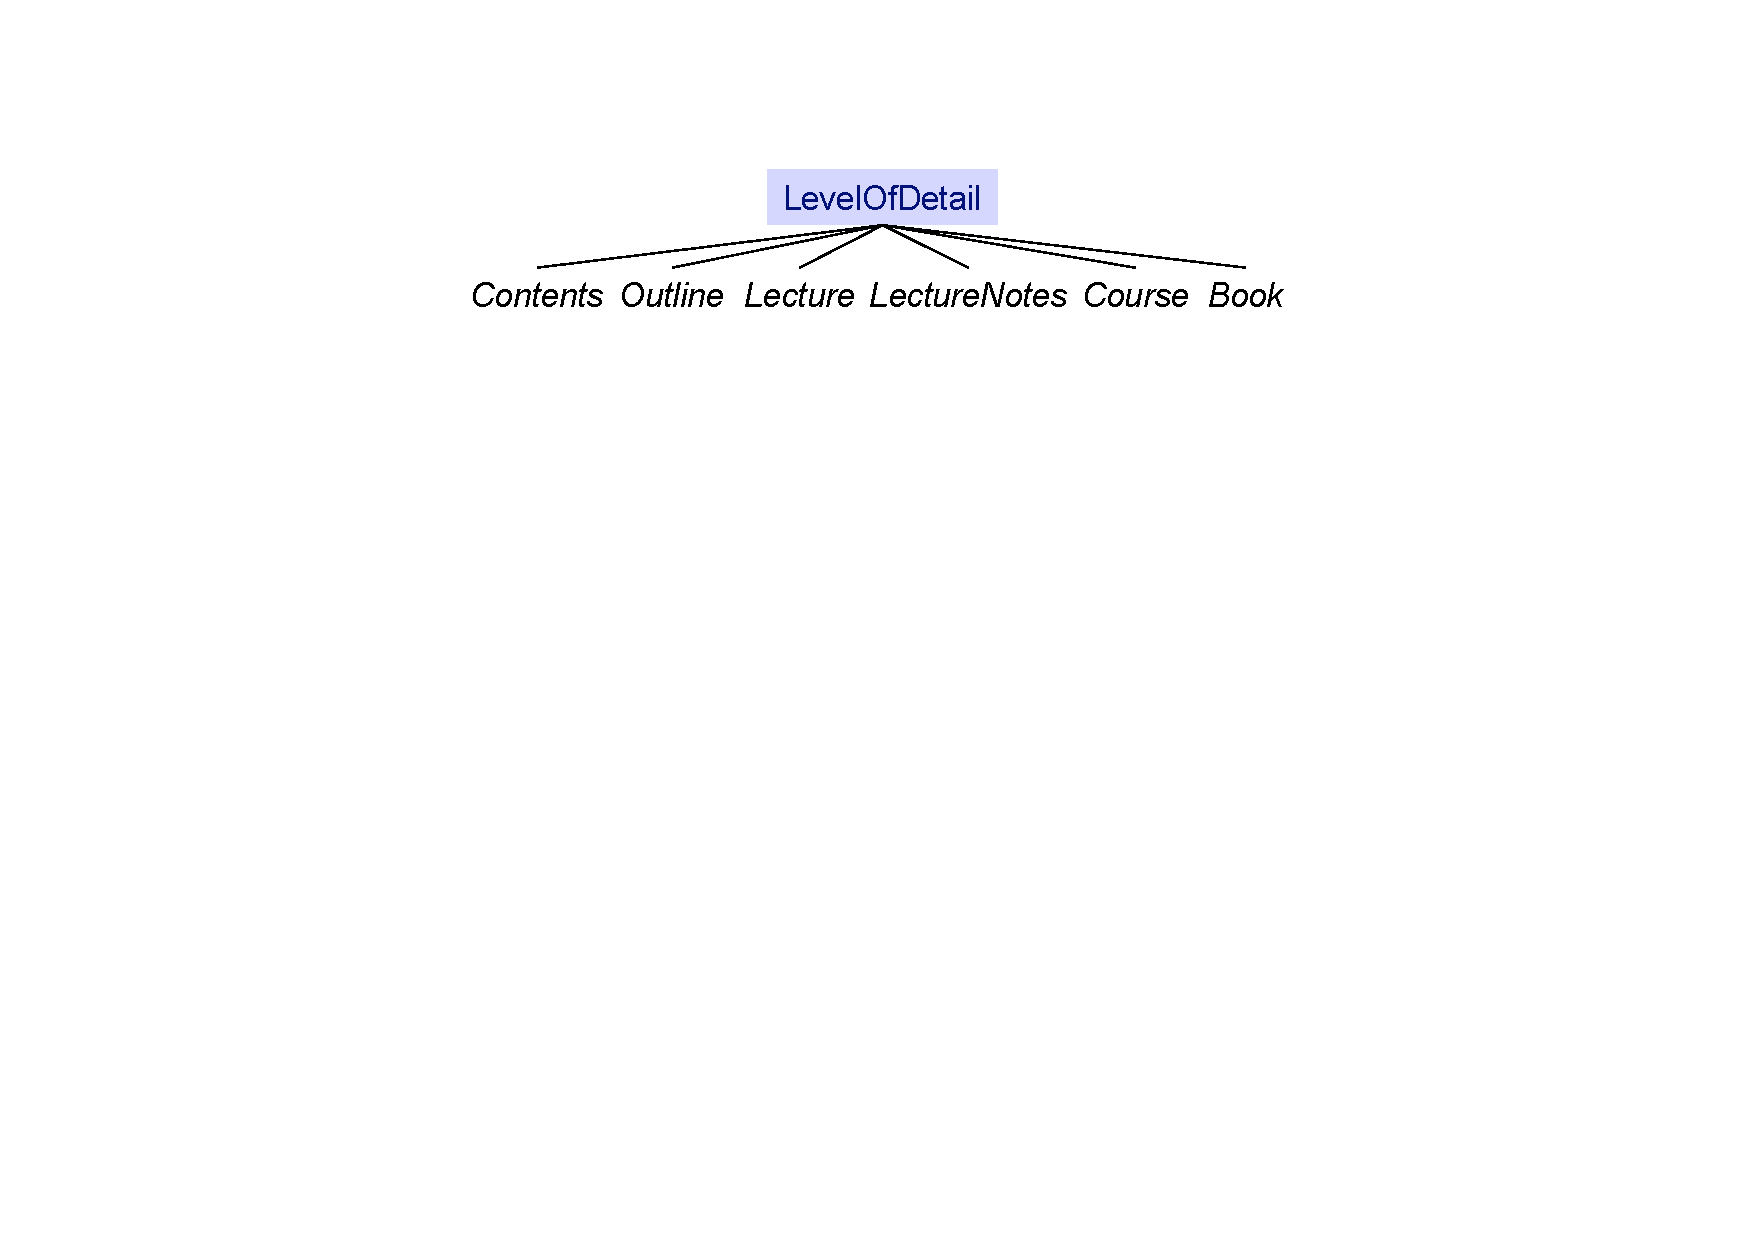
\includegraphics[width=\textwidth]{img/LevelOfDetailAttr}
    \caption{Level of Detail Attributes.}
    \label{fig:LevelOfDetailAttr}
  \end{center}
\end{figure}

develop transparencies, lecture notes, complete courses
\DefObject{LectureAttribute}{\LectureAttribute}


\BKB{to be edited}
Different levels of detail for the {\`O}same{\'O} structural element appear as distinct elements with the same Id (see Variant Attributes above). Note, however, that sub-elements may be shared (by Include), e.g. \ExampleStr{}s, \DefinitionStr{}s, etc.

%Contents
%Content skeleton containing Titles only. Usually generated as a View, see below.
%<<thus maybe not needed as an attribute, only as an option for views?>>
%Outline
%Outline skeleton containing \AbstractStr{}s only. Usually generated as a View, see below.
%<<thus maybe not needed as an attribute, only as an option for views?>>
%Lecture
%Overheads (including material such as \ExampleStr{}s or tool sessions) suitable for presentation in class.
%Lecture Notes
%Lecture Overheads, augmented by comments, further explanations, \ExampleStr{}s, etc. such that the document is suitable for study after it has been presented in class.
%Course 
%Lecture Notes, augmented by further material (e.g. expanding overheads into textual ParagraphStrs) such that the document is suitable for self-study as an electronic hyper-document (on-line or off-line, resp.).
%Book
%Course Material in a completely textual version, suitable for publication as a book.
%<< not to be included here? >>
\end{Paragraph}
\end{Section}

\begin{Section}[Title={Interaction Levels},Label={Interaction_Levels}]
\begin{Paragraph}
%\subsubsection{Interaction Levels}

\begin{figure}[htbp]
  \begin{center}
    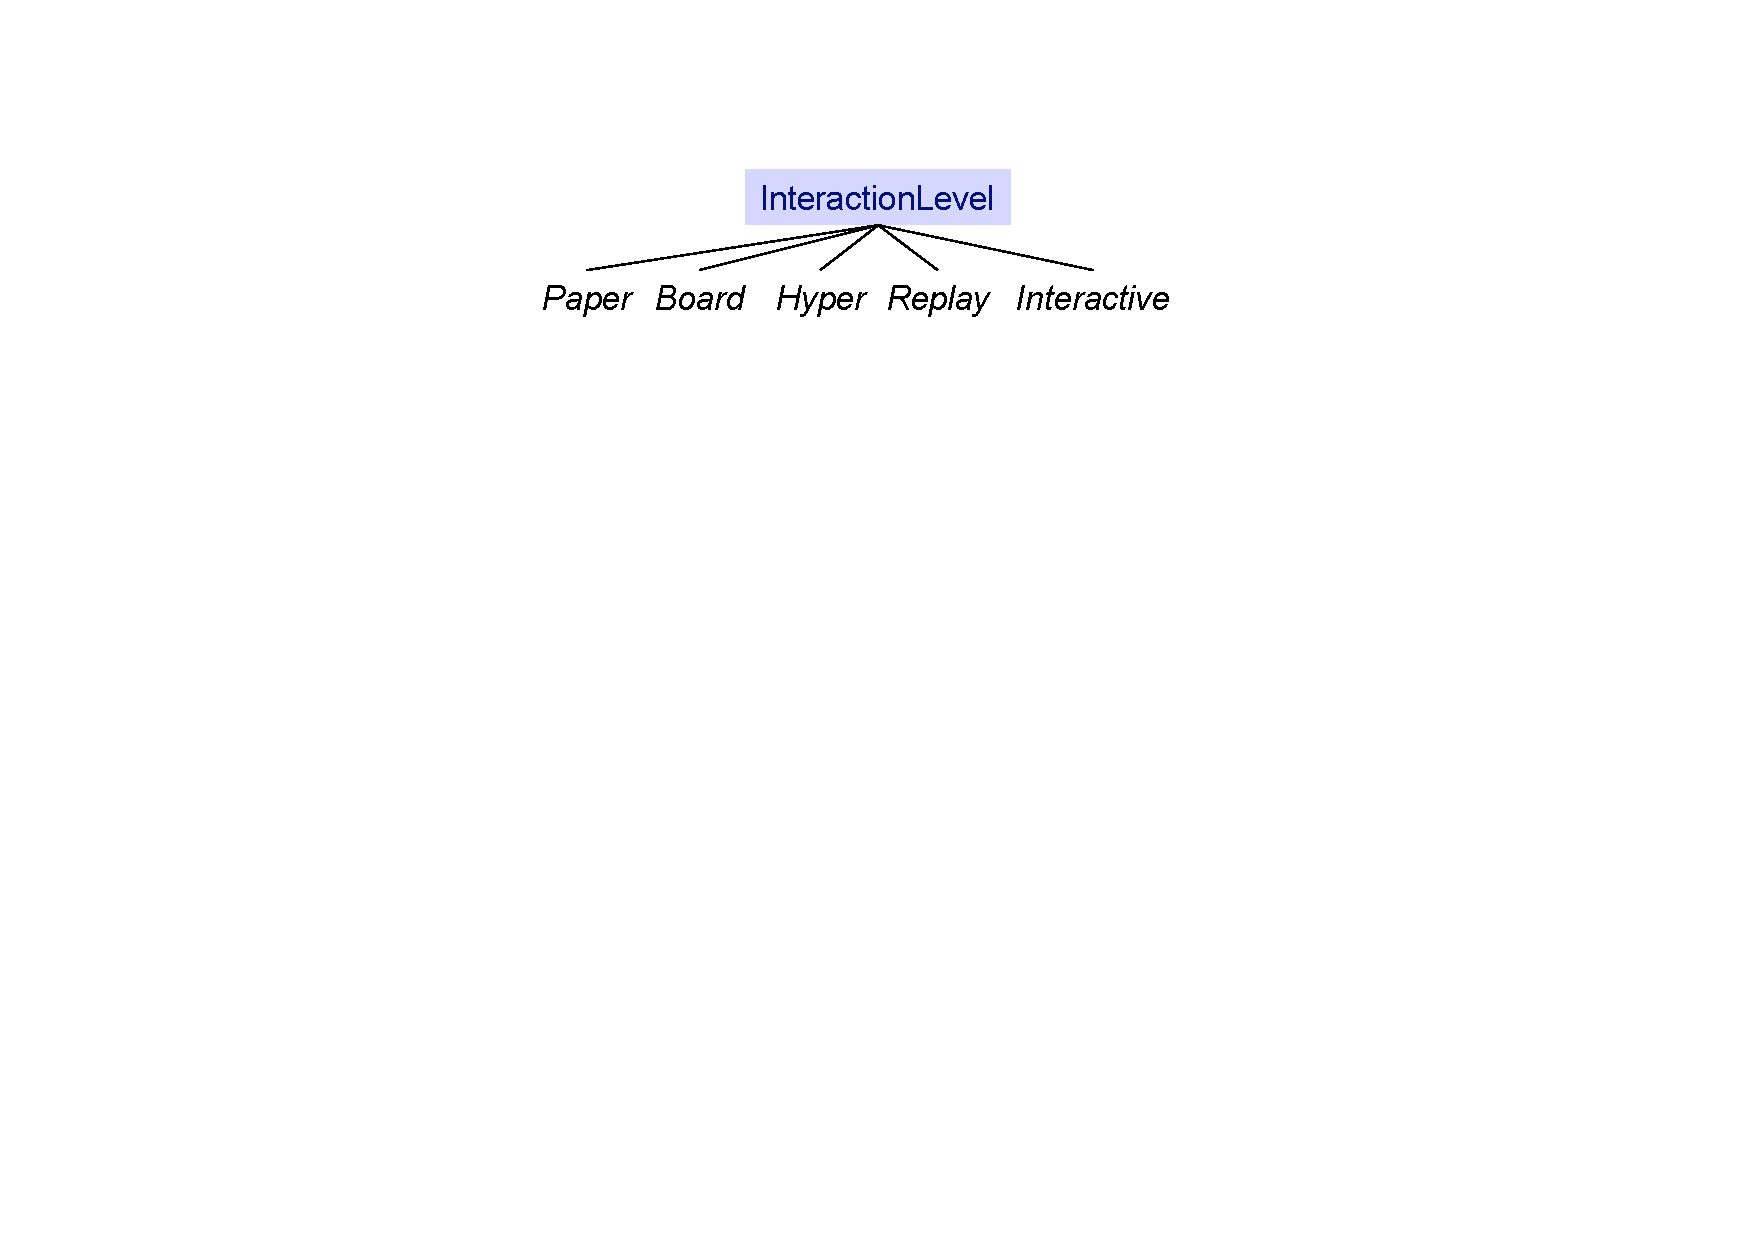
\includegraphics[width=\textwidth]{img/InteractionLevelAttr}
    \caption{Interaction Level Attributes.}
    \label{fig:InteractionLevelAttr}
  \end{center}
\end{figure}


\begin{figure}[htbp]
  \begin{center}
    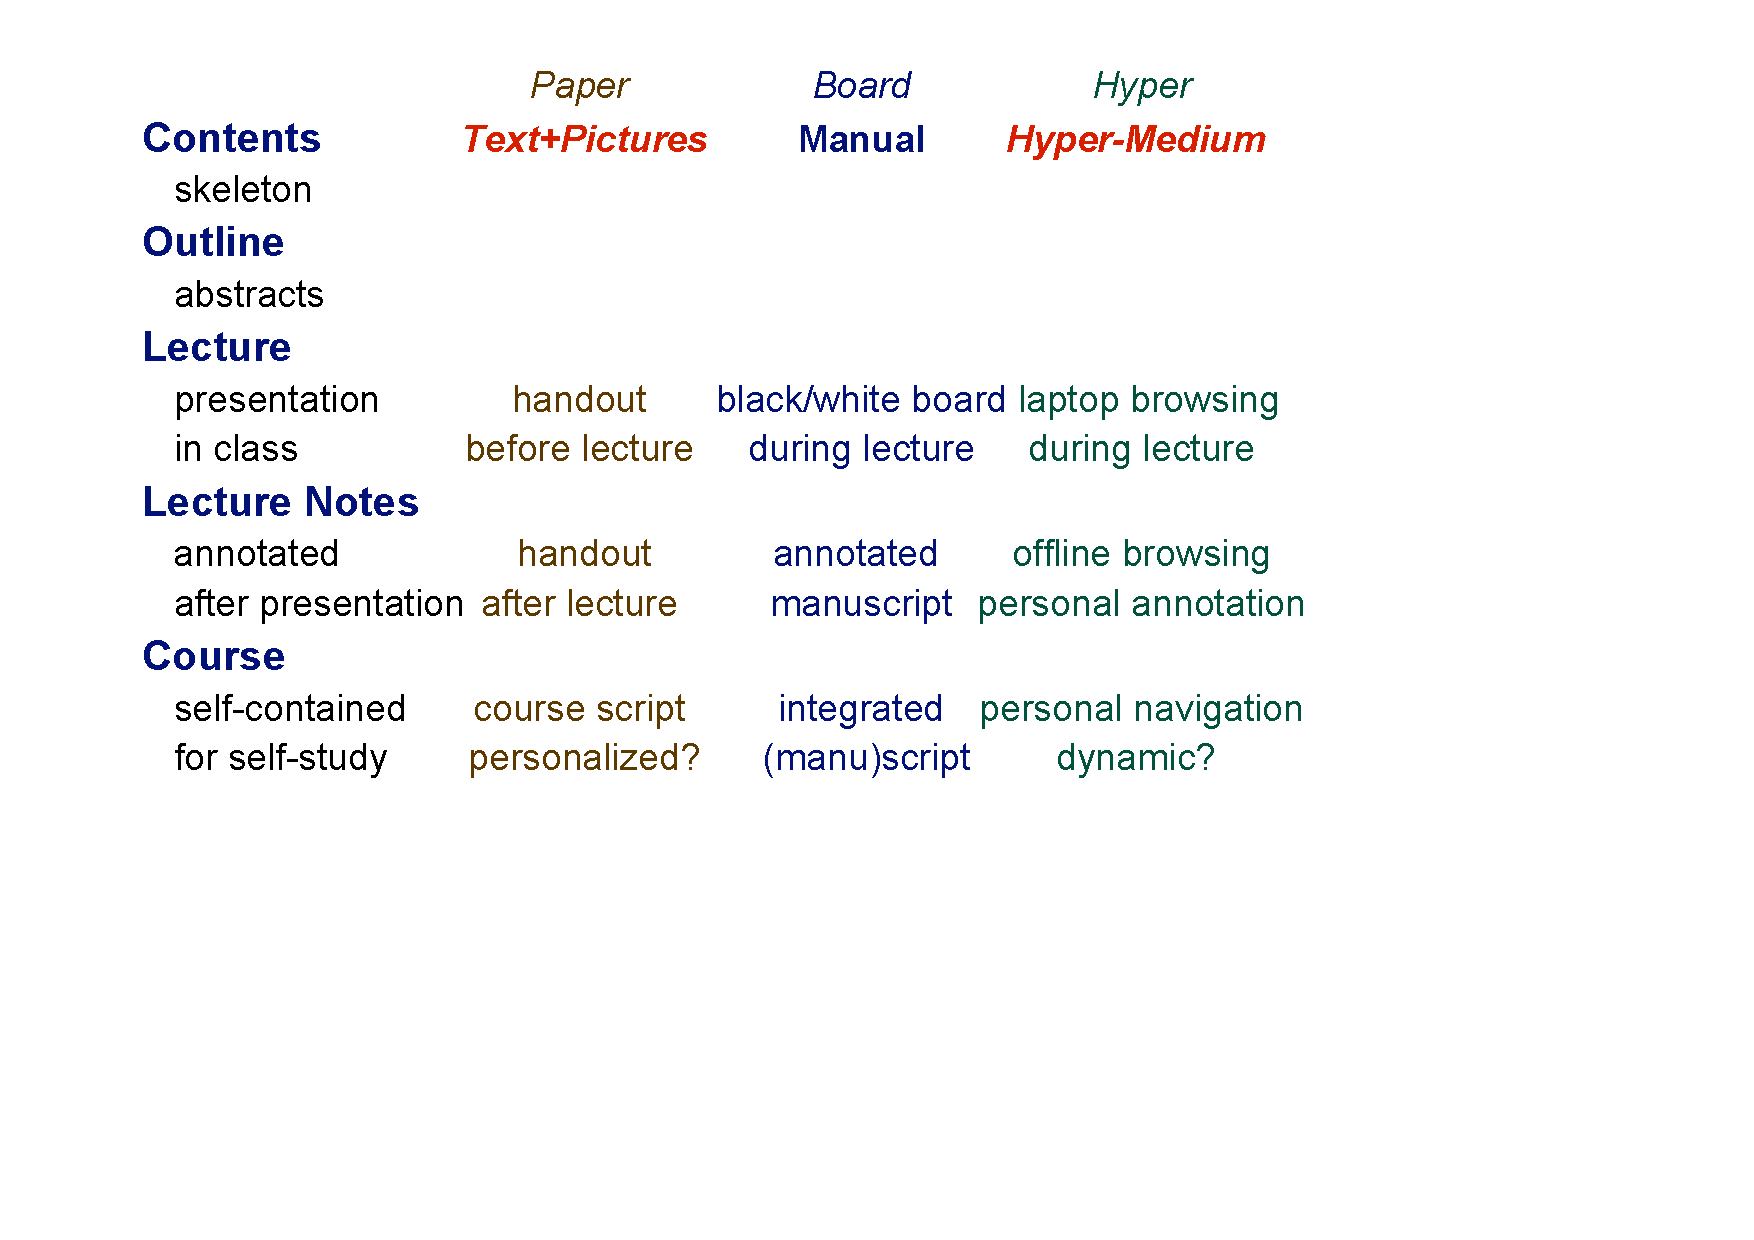
\includegraphics[width=\textwidth]{img/PaperBoardHyper}
    \caption{Interaction Levels Paper, Board, and Hyper.}
    \label{fig:PaperBoardHyper}
  \end{center}
\end{figure}

\begin{figure}[htbp]
  \begin{center}
    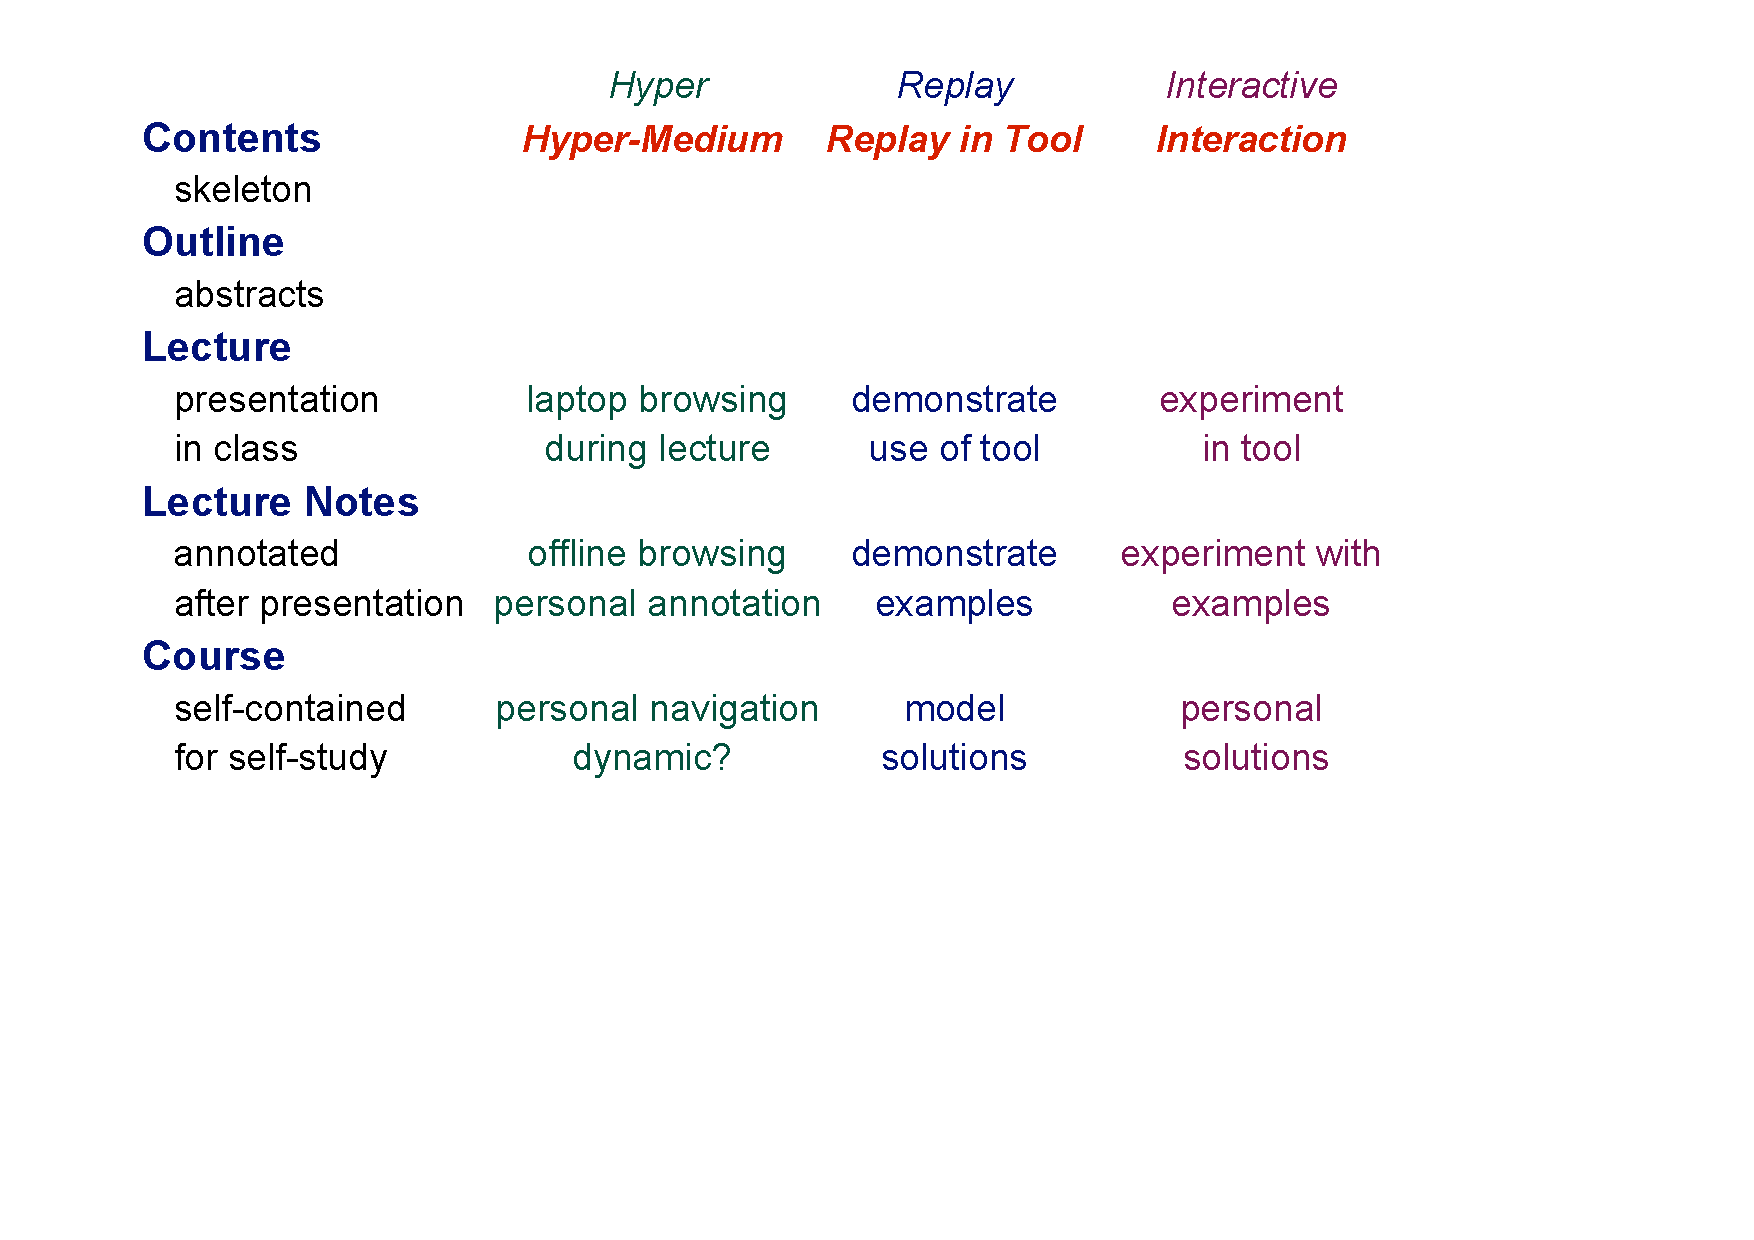
\includegraphics[width=\textwidth]{img/HyperReplayInteractive}
    \caption{Interaction Levels Replay and Interactive.}
    \label{fig:HyperReplayInteractive}
  \end{center}
\end{figure}

work on the board, with transparencies, interactively with tools
\end{Paragraph}
\end{Section}

\begin{Section}[Title={Use of Tools},Label={Use_of_Tools}]
\begin{Paragraph}
%\subsubsection{Use of Tools}
\end{Paragraph}
\end{Section}

\begin{Section}[Title={Views},Label={Views}]
\begin{Paragraph}
%\subsubsection{Views}
\label{sec:views}
\end{Paragraph}

\end{Section}
\end{Section}

\begin{Section}[Title={Semantic Interrelation},Label={Semantic_Interrelation}]
%\subsection{Semantic Interrelation}

\begin{Section}[Title={Ontology},Label={Ontology}]
\begin{Paragraph}
%\subsubsection{Ontology}
agree with your colleague on a  uniform terminology
\end{Paragraph}
\end{Section}

\begin{Section}[Title={Semantic Elements and Categories},Label={Semantic_Elements_and_Categories}]
\begin{Paragraph}
%\subsubsection{Semantic Elements and Categories}

\begin{figure}[htbp]
  \begin{center}
    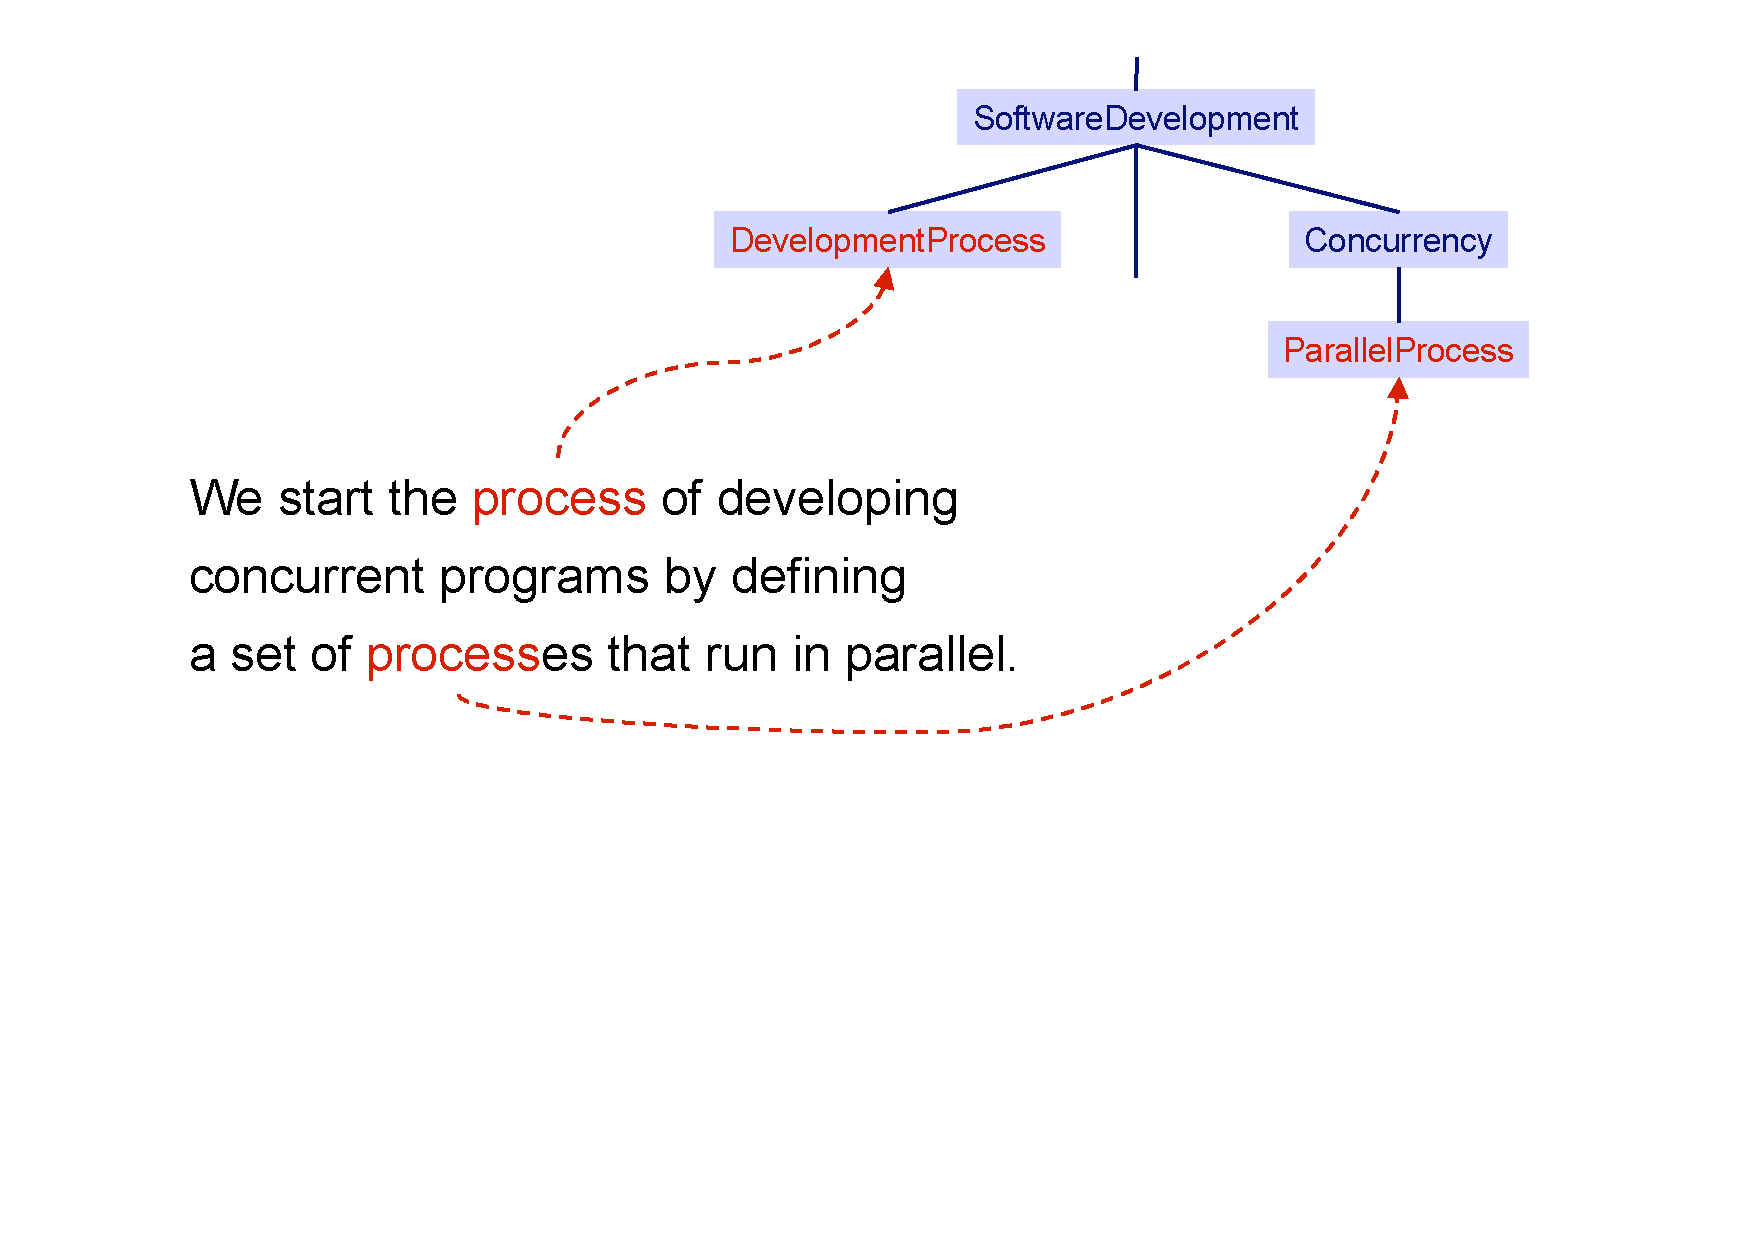
\includegraphics[width=\textwidth]{img/ProcessExample2}
    \caption{References to Two Different Semantic Elements.}
    \label{fig:ProcessExample2}
  \end{center}
\end{figure}

\ReferenceStr{}s. 


\BKB{to be edited}
%2.8.1 Define Element
%Label: ElementId       Body: Text
%The semantic element is defined: the position of its {\`O}defining occurrence{\'O} is given (the Label must always be provided) that will be referred to via a hyper-link in a Reference; the ElementId is used in a Reference; the Body will be displayed in any Reference to it. 
%The semantic element should first be defined in the ontology, in an associated ontology editor (to be developed); then consistency checking w.r.t. the ontology becomes possible. 
%Note that a Semantic Element can also be used to give a proper Name to a (mathematical) symbol, or several to discriminate overloading; in contrast to a Semantic Category (see below), a hyperlink is created here for each Reference.
%As examples consider 
%       {\^O}Define(DevelopmentProcess,process){\~O} 
%       {\^O}Define(CSP-Process,process){\~O}
%       {\^O}Define(IntPlus,+){\~O} 
%       {\^O}Define(MatrixPlus,+){\~O}
%       {\^O}Define(Hearts,heartssymbol){\~O}   
%[hearts symbol corresponds to a LaTeX macro, until layout attributes become available]
%2.8.2 Reference
%Element: Name  RefText: [Text]
%The semantic element given by its Name is represented by the Body given where it is defined  and, for the Interaction Level PAPER, a textual reference to a page number, otherwise a hyper-link (depending on the tool support environment, the hyper-link may have the option of accessing a correspon-ding Glossary Entry for this Name as an alternative, e.g. via the right mouse button). The optional RefText, if provided, is presented as an (overriding) alternative text, containing the hyper-link. 
%As an example consider {\^O}Reference(DevelopmentProcess){\~O}, presented as {\^O}process{\~O} in the text (with an underlying hyper-link); this allows for an internal semantic disambiguation of an otherwise overloaded terminology in the displayed text{\~N}thus the correct reference is provided in each case.
%[Note that in the MMiSS-Latex input, {\^O}Reference(Hearts){\~O} can be abbreviated as just Hearts]
%Alternatively, with an explicit RefText, {\^O}Reference(DevelopmentProcess, development process){\~O} is presented as {\^O}development process{\~O} in the text (with an underlying hyper-link).
%The element must have occurred previously (e.g. it must have been defined); this will be checked by tools (cf. also the section about Order).
%Variant attributes specify the particular variant of the Name (the goal); they only have to be given, if they differ from the inherited ones at this point.
%2.8.3 Forward Reference
%Element: Name  RefText: [Text]
%Same as Reference, except that the element need not have occurred previously. Tools will check that it is indeed defined (possibly later) such that no {\`O}dangling references{\'O} occur.
%2.8.4 Define Category
%Category: Id   NumberParameters: Number        Body: Text
%A Category is associated with an entry in the ontology (which must have been previously defined). 
%A new Category inherits all attributes from its ancestor in the ontology hierarchy, if any; new attributes, in particular LayoutAttr, may be defined for it.
%A Category with no parameters ({\`O}constant category{\'O}) is analogous to a Semantic Element: in a Category Reference, the text of the defining occurrence is substituted (as for a Semantic Element), but no hyperlink is provided. Note that this feature can also be used to give a proper Name to a (mathematical) symbol, or several to discriminate overloading (cf. Semantic Elements). 
%A Category may have one or more parameters. The parameters may be referred to in the Body by ordinal number, i.e. {\^O}{\#1}{\~O} refers to the first parameter in the Category Reference. 
%As examples consider 
%       {\^O}DefineCategory(High,1,RED(#1)){\~O}        
%       {\^O}DefineCategory(Low, 1,GREEN(#1)){\~O}      
%       {\^O}DefineCategory(Quotation, 1,SMALL(#1)){\~O}        
%       {\^O}DefineCategory(Rule, 2,LEFT(#1) CENTER({\DH}>) RIGHT(#2)){\~O}         
%[in the above, RED, GREEN, {\'E} should correspond to layout commands in LaTex, to be used instead of Layout Attributes until these become available]
%2.8.5 Category Reference
%Category: Name         Parameters: {Text}
%A Text marked by a specific Category Reference is linked to the ontology and may yield a special presentation. An actual parameter text must be given for each formal parameter, to be substituted as prescribed in the Category Definition.
%As examples consider 
%       {\^O}Category(High,this one here){\~O}  -- this one here
%       {\^O}Category(Low, this other one){\~O} -- this other one 
%       {\^O}Category(Quotation, this is a quote){\~O}  -- this is a quote 
%       {\^O}Category(Rule, A,B){\~O}   -- A     ->     B)
%[Note that in the MMiSS-Latex input, {\^O}Category(High,this one here){\~O} can be abbreviated as just {\^O}\High{this one here}{\~O}, and {\^O}Category(Rule, A,B){\~O} as {\^O}\Rule{A}{B}{\~O}]
\end{Paragraph}
\end{Section}

\begin{Section}[Title={Packages},Label={Packages}]
\begin{Paragraph}
%\subsubsection{Packages}
\label{sec:packages}
% \BKB{CXL: etwas ueber Packages und import hier? ergaenzt durch BKB}

\emph{Packages} provide a means for modular document development by
introducing \emph{name spaces}. When writing a document, authors
introduce identifiers to refer to structural elements, semantic
elements, and categories. If these identifiers, subsumed as \emph{names}
in the following, are defined more than once, we say there is a
\emph{name clash}. 

A package encapsulates the name space of a document, such that names
defined in package do not clash with names from other packages. In
order to use names from other packages, these have to be imported
explicitly. In other words, packages are very much like modules in
programming languages such as Modula-2, Haskell, or Java. 


\paragraph{Package Hierarchy.}
%
Packages are organised in a hierarchical folder structure, with the
names given by \emph{paths}. Because path names can get very long,
paths can be renamed by \emph{path aliases} of the form 
$$\mathtt{a} = \mathtt{p}_1.\mathtt{p}_2. \ldots. \mathtt{p}_n $$
where \texttt{a} is the new alias, and
$\mathtt{p}_1$,\ldots,$\mathtt{p}_n$ are either folder names or
previously defined aliases, subject to the condition that each alias
is defined exactly once, and alias definitions are acyclic.

There are three \emph{special aliases}: \texttt{Current} refers to the
folder of the package it is used in; \texttt{Parent} refers to the
parent folder; and \texttt{Root} refers to root folder of the folder
hierarchy. (Thus, the three special aliases correspond to
`\texttt{.}', `\texttt{..}' and `\texttt{/}' in Posix systems.)  Users
are discouraged to use the \texttt{Root} alias, since it makes
reorganising the folder hierarchy difficult; it is mainly intended for
usage by tools.

\paragraph{Export and Import.}
%
The local names are the ones defined in this package (as opposed to
\MarginComment{JGS: ``imported into package'' $\to$ `imported into the package''?}
the ones imported into package).  By default, all local names are
exported. It is not possible to restrict the export further (although
we can reexport imported names); rather, name clashes are resolved on
import. 

A package specifies the imported packages in the \emph{import
  preamble}. The import preamble contains a number of import clauses,
which specifies a package to be import, plus a number of \emph{import
  directives}. Import directives allow us to specify:
\begin{itemize}
  \item Path aliases;
  \item Local or global import (when importing globally, the imported
    names are re-exported);
\MarginComment{JGS: ``when import qualified''? Grammatik!}
  \item Qualified or unqualified import (when import qualified, the
    imported structural identifiers are prefixed with the name of the
    package from which they are imported);
  \item Hiding, revealing, or renaming of imported names (when we hide
    a name, it is not imported; when we reveal names, only these are
\MarginComment{JGS: Semikolon fehl am Platz}
    imported);
\end{itemize}
\end{Paragraph}
\end{Section}
\end{Section}

\begin{Section}[Title={Sustainable Development for Re-use},Label=s25]
\begin{Paragraph}
%\subsection{Sustainable Development for Re-use}
 (partially) re-use the transparencies of a colleague
re-use, sharing, views
\end{Paragraph}
\begin{Section}[Title={Order},Label={Order}]
\begin{Paragraph}
%\subsubsection{Order}
\label{sec:order}
use order only when necessary

\Hidden{
Note that the order of the \Node{}s in the \Graph{} is not semantically
relevant (in particular, the order of the four \ParagraphStr{}s making up
the main part of the section). Of course, when \emph{presenting} the
document the order may become relevant, since some presentations (such
as slides for lecture series, or text in the corresponding textbook)
have an implicit linear order; but for example, in a hypermedial
presentation which allows the user to navigate freely, sections may
not appear in any fixed order.
}

\BKB{Rest der Section muss durch BKB noch mit den anderen Teilen zusammen gefuehrt werden}
\end{Paragraph}
\end{Section}

\begin{Section}[Title={Change Management},Label={Change_Management_1}]
\begin{Paragraph}
%\subsubsection{Change Management}
be made aware of the changes made by your colleague
(cf.  Sect.~\ref{sec:change-management})
\end{Paragraph}
\end{Section}

\begin{Section}[Title={Versions, Configurations},Label={Versions_and_Configurations}]
\begin{Paragraph}
%\subsubsection{Versions, Configurations}

\begin{figure}[htbp]
  \begin{center}
    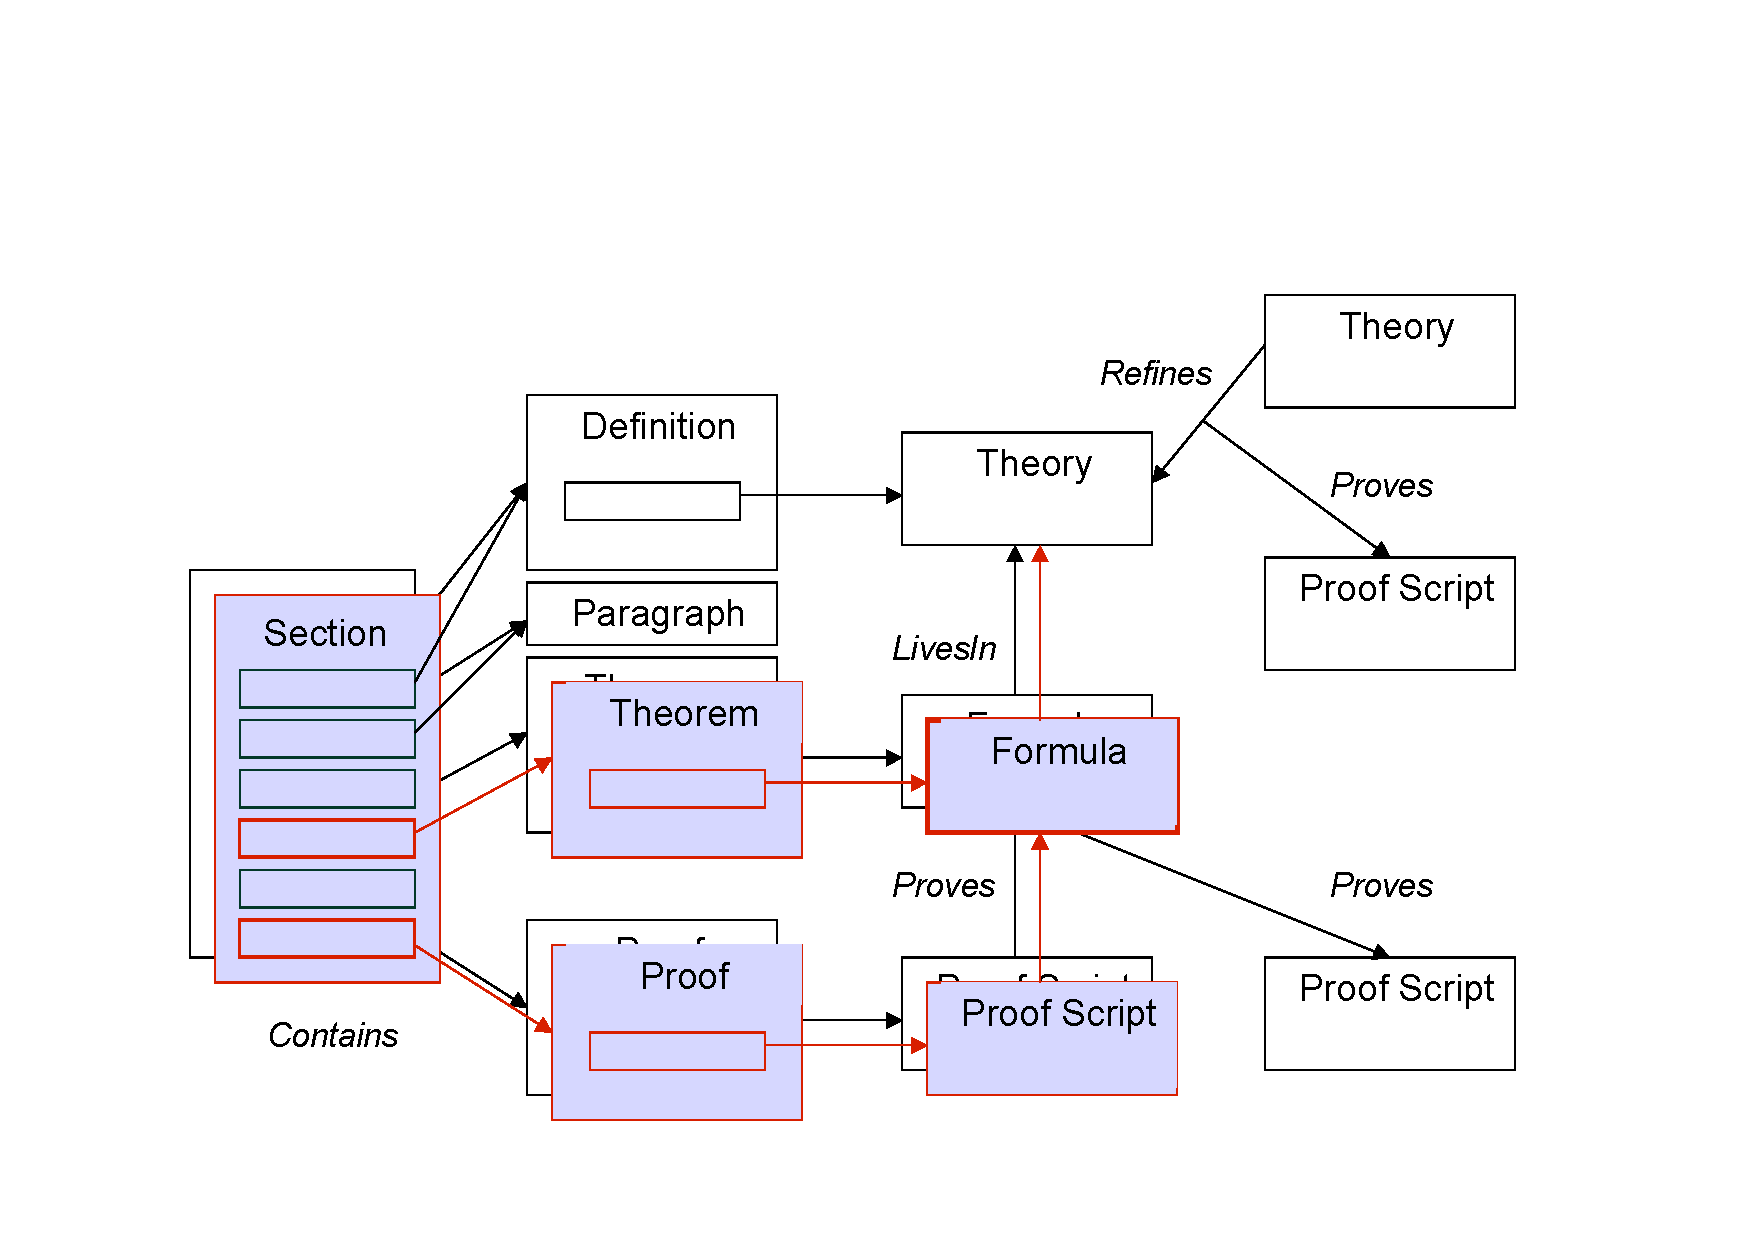
\includegraphics[width=\textwidth]{img/ExConfigurations3}
    \caption{Example of New Version and Configuration.}
    \label{fig:ExConfigurations3}
  \end{center}
\end{figure}
\end{Paragraph}
\end{Section}

\begin{Section}[Title={Consistency and Completeness},Label={Consistency_and_Completeness}]
\begin{Paragraph}
%\subsubsection{Consistency and Completeness}
publish complete and consistent {\~a}packages{\`O}
\end{Paragraph}
\end{Section}
\end{Section}

\end{Section}

% The support environment 
\begin{Section}[Title={The Support Environment},Label={The_Support_Environment}]
\begin{Paragraph}
%\input{architecture.tex}
%\section{The Support Environment}
\label{Support-Environment}
\RevisedBy{BKB 030426}


This section gives an overview of the \DefClass{SupportEnvironment}{\SupportEnvironment}
%       teaching and learning environment 
\BKB{APH: ich ziehe Support Env vor, nicht ganz so anspruchsvoll}
that integrates the authoring, management,
and presentation tools for documents.
It sketches the goals of such an environment and describes
the main components of the architecture and their relation.
More details about the central components are contained in
Sect.~\ref{sec:repository} and Sect.~\ref{sec:presentation}.

%\subsection{Goals}
%\Authors{A. Poetzsch-Heffter}
\end{Paragraph}
\begin{Section}[Title=Goals,Authors={A. Poetzsch-Heffter},Label=s31]
\begin{Paragraph}
Teaching and learning based on multimedia documents can only
be done with the help of a computer-supported environment.
The \SupportEnvironment{} that we develop in the
\MMiSS{} project aims at three major and two minor goals.
The major goals are to support:
\begin{description}
\BKB{APH, CXL: hier Vorschlag fuer Ueberarbeitung der Kategorien}

%       \item [Development]
\item [Authoring]
The \AuthorRole{}s should be particularly supported in the development
of course material, i.e. the production of
new \Doc{}s (viz. \PackageStr{}s) and the adaption, composition and \Revision{} of existing
ones.

%       \item [Content management]
\item [Development]
Development management is responsible for persistency and
accessibility of the material (\Repository{}), and it has to treat \VersionControl{}, \ConfigurationManagement{} and \ChangeManagement{}
(\DevelopmentManager{}) for \ConsistencyConf{} and
the dependencies between the document components (via the \Ontology{}). 
%       Furthermore, it helps to integrate external components into documents.
\BKB{APH, DH: siehe auch unten: Integration of Foreign Tools}

\item [Usage and Interaction]
The use of the learning material will be supported in different kinds of
teaching scenarios: by a \TeacherRole{}, \TutorRole{} or \StudentRole{}  on various \PresentationPlatform{}s, or for individualised self-study by a \StudentRole{} using \ActiveMath{} (see Sect.~\ref{sec:activemath}).
Moreover, \StudentRole{}s and \CorrectorRole{}s use \WebAssign{} for assignments (see below).
%       It can not only mean
%       the presentation of the material by a teacher. But as said
%       in the overview, we aim at more ambitious support, in particular
%       at an intelligent tutoring environment.
\end{description}

The minor goals are a flexible user management with
administration support 
and the possibility for integrating
typical tools for electronic communication.
\BKB{APH: was soll das sein bzw. realistisch noch werden? besser: future integration with local environments such as UPortal?}


%\subsubsection{Architecture}
\end{Paragraph}
\begin{Section}[Title=Architecture,Authors={D. Hutter, C. L�th},Label=s32]
\begin{Paragraph}
\label{sec:architecture}
%\Authors{D. Hutter, C. L\"uth}
\BKB{APH, CXL: es sollte nur ein Bild des Environments geben; bitte einigt Euch auf eine gemeinsame Ontologie (siehe Vorarbeit von mir)  -- evtl. in Fulda zur Not (aber viel Zeit ist nicht mehr) -- und ein Bild, nicht so riesig wie das von APH, evtl. ohne Legende}

\begin{figure}[htbp]
  \begin{center}
    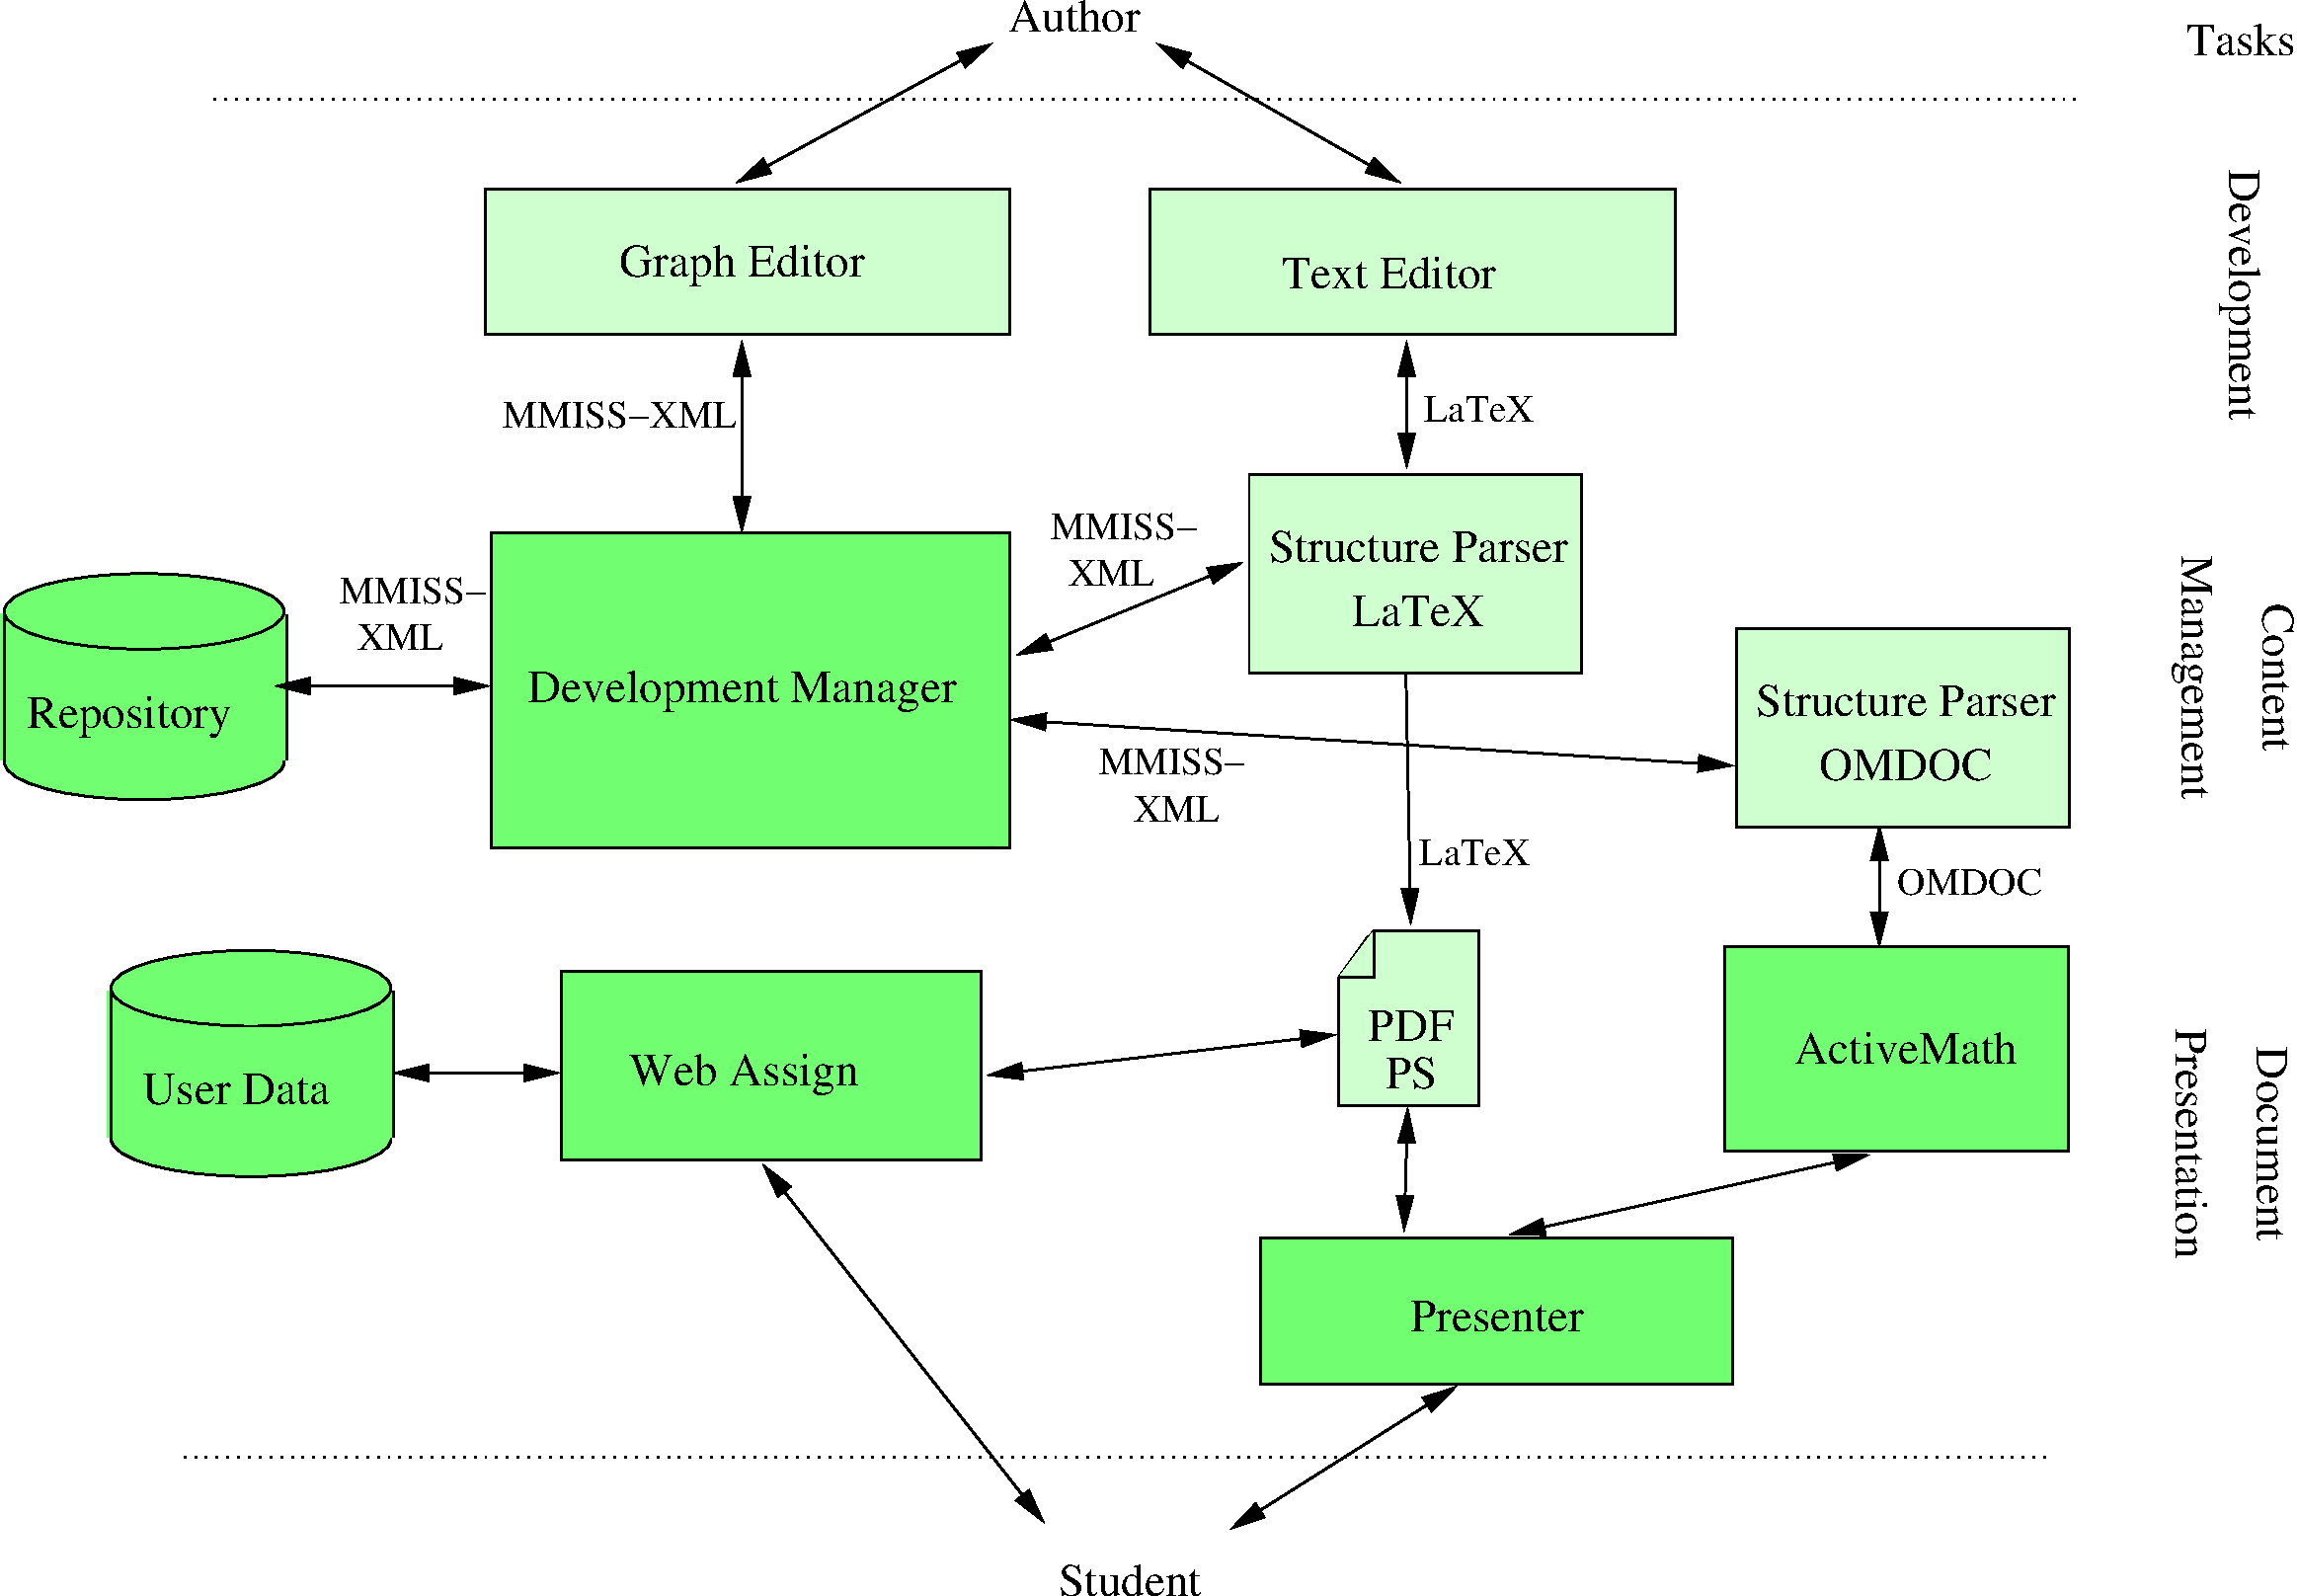
\includegraphics[width=\textwidth]{img/repository-sysarch}
    \caption{MMiSS Support Environment System Architecture}
    \label{fig:repository-sysarch}
  \end{center}
\end{figure}

\Authors{A. Poetzsch-Heffter}
%\begin{figure}[hbtp]
%\centerline{\includegraphics[scale=0.4,angle=90]{img/architecture}}
%The arrows represent action calls, as follows:\\
%1: get/put teaching material components, get view of repository\\
%2: read/write access to database\\
%3: get teaching material\\
%4: get/put teaching material items\\
%5: get assignments\\
%6: activate\\
%7: send/receive messages\\
%8: data exchange
%\caption[ ]{Architecture of the Support Environment}
%\label{fig-architecture}
%\end{figure}
%\BKB{wie erreiche ich, dass die Fig NICHT auf einer eigenen Seite erscheint?}


\BKB{Texte zusammen gefuehrt; erweitern?}
To achieve the above goals we have designed an open,
web-based architecture 
\BKB{APH: inwiefern web-based?}
that integrates subsystems developed
by the different partners. 
Figure~\ref{fig-architecture}
shows the major components of the \SupportEnvironment{}. 
%Fig.~\ref{fig:repository-sysarch} shows the system architecture of the
%\Repository{} and {\DevelopmentManager}. 
The \Repository{} holds the \StructureGraph{}s of documents
and provides 
{\VersionControl}{version control} and
{\ConfigurationManagement};
the {\DevelopmentManager}  implements {\ChangeManagement}. 
\BKB{Achim, CXL: ist das so? siehe Ontologie}

The \GraphEditor{}, i.e. the user interface to the \DevelopmentManager{}, and the \TextEditor{} constitute the major \AuthoringTool{}s.

\Authors{A. Poetzsch-Heffter}
%       The core of the system is the \emph{repository}
%       that is responsible for the content management. It
%       manages and visualizes the document components, their
%       versions, relations, and dependencies. It provides
%       a programming interface to access and modify
%       components. \emph{Authoring tools} use this interface to
%       communicate with the repository. They help with the development
%       of the content and semantic integration of new documents into
%       the base of existing material. 
%% BKB: m.E. schon gesagt, evtl aufgreifen, wenn an anderer Stelle oder oben integrieren
%       A naming mechanism is
%       used to link \emph{external components and tools} into courses.
%       Such components can range from simple applets to
%       full-blown theorem provers.
%% BKB: verstehe ich nicht; nichts versprechen, was wir nicht halten

%       Currently the architecture of the environment provides three
%       different subsystems to present and work with the documents.
%       As simple \emph{presentation platforms}, we use ordinary web-browsers
%       and reader tools.
%       \emph{ActiveMath} is a learning environment for its own.
%       It is being developed mainly at the DFKI in Saarbr\"ucken and
%       partly at the university of Saarbr\"ucken.
%       Its outstanding features are:
%       \begin{itemize}
%       \item
%       individualized learning in a user-adaptive environment
%       based on a explicit user model,
%       \item
%       active learning by integrating external tools into the
%       work process enabling exploratory learning, pedagogically
%       motivated presentation, and some new proof planning
%       aspects.
%       \end{itemize}

%       ActiveMath is described in detail in Sect.~\ref{sec:activemath}.
%% BKB: kommt spaeter ausfuehrlicher


%%%%%%%%%%%%%%%%%%%%%%%%%%%%%%%%%%%%%%%%%
% Repository, Authoring Tools and Development Management -- C. Lueth, D. Hutter
%\input{repository.tex}
\end{Paragraph}
\begin{Section}[Title={The Repository},Authors={D. Hutter, C. L�th},Label=s33]
\begin{Paragraph}
%\subsection{The Repository}
\label{sec:repository}
%\Authors{D. Hutter, C. L\"uth}
\RevisedBy{BKB 030423 (considerably)}

The \MMiSS{} 
\DefClass{Repository}{\Repository}, 
is the central database maintaining \MMiSS{}
documents. Authors can add, modify or change documents using an
\AuthoringTool{} while 
\SustainableDevelopment{} is supported by fine-grained
{\VersionControl},
{\ConfigurationManagement} and a
{\ChangeManagement} in the
{\DevelopmentManager}. 
\end{Paragraph}
\begin{Section}[Title={Representation of Structured Documents},Label={Representation_of_Structured_Documents}]
\begin{Paragraph}
%\subsubsection{Representation of Structured Documents}

The \MMiSS{} \Repository{} stores and retrieves \MMiSS{} documents,
structured as outlined in
Sect.~\ref{Sec-SemanticDocumentStructuring}. Thus, the
\DefClass{RepositoryObject}{\RepositoryObject}s 
in the \Repository{} are 
\StructuralEntities{}  such as {\SectionStr}s, {\ProgramStr}s, {\ExerciseStr}s,
{\TextFragmentStr}s etc. These \RepositoryObject{}s are related, most obviously by textual nesting, but
also by 
%explicit or implicit
\LinkStr{}s or \ReferenceStr{}s. 
%An example of an explicit structural link is a reference; an
%example of an implicit structural link is using a semantic category.
\end{Paragraph}
\end{Section}
\begin{Section}[Title={Structure Graph},Label={Structure_Graph}]
\begin{Paragraph}
%\subsubsection{Structure Graph}
\label{sec:structure-graph}
This structure gives rise to the 
\DefClass{StructureGraph}{\StructureGraph}, 
which has the
\RepositoryObject{}s as \Node{}s, and the relations as labelled, directed \Edge{}s.
With regard to the \Contains{}{}{} relation, the \Graph{} is directed and
acyclic, but it is not a tree, since \StructuralEntities{}  may be included in more
than one place (\StructuralSharing{}). The structured representation as
a \Graph{} allows operations to take the structuring into account (see e.g.
{\ChangeManagement} described in 
Sect.~\ref{sec:change-management}). 
It is also the basis for 
{\ConfigurationManagement}
when considering {\VersionControl}, leading to
the notion of a  {\DevelopmentGraph} (see
below).

\BKB{als Beispiel w\"urde ich noch lieber Bestandtteile dieses Papers oder 
von Folien dazu nehmen; evtl. bekommen wir das noch hin}
As an example, consider a %chapter out of a 
real-life lecture series
introducing formal program development in the algebraic specification
style to undergradute computer science students
\cite{roba:FormProgDev}. One section of this lecture series,
corresponding roughly to one lecture, introduces the basic concepts of
algebraic specifications. The document is structured as follows:

\begin{itemize}
\item it has a short {\IntroductionStr} motivating what is going to come
\item an {\AbstractStr} summarising the new concepts 
\item the main part consisting of {\ParagraphStr}s
introducing and defining 
the concepts of 
\Signature{}s, \Algebra{}s, and \Term{}s,
\item followed by a short {\ExampleStr}
  (the natural numbers in CASL),
\item and closes with a {\SummaryStr} of the new concepts 
\end{itemize}

{\IntroductionStr} and {\SummaryStr} contain a list
enumerating the concepts the user is about to learn, or has just learned. The main parts are
{\ParagraphStr}s, which are structured further: for example,
\Signature{}s, 
{\Algebra} and {\Term}s contain
definitions of the corresponding concept. 
The resulting \StructureGraph{} is shown in
Fig.~\ref{fig:example-doc-graph}.
Note how later \DefinitionStr{}s
and \ExampleStr{}s refer back to earlier \DefinitionStr{}s
(indicated by dashed arrows), for example to define
an \Algebra{} we need to refer to \Signature{}s. 

\begin{figure}[htbp]
  \begin{center}
    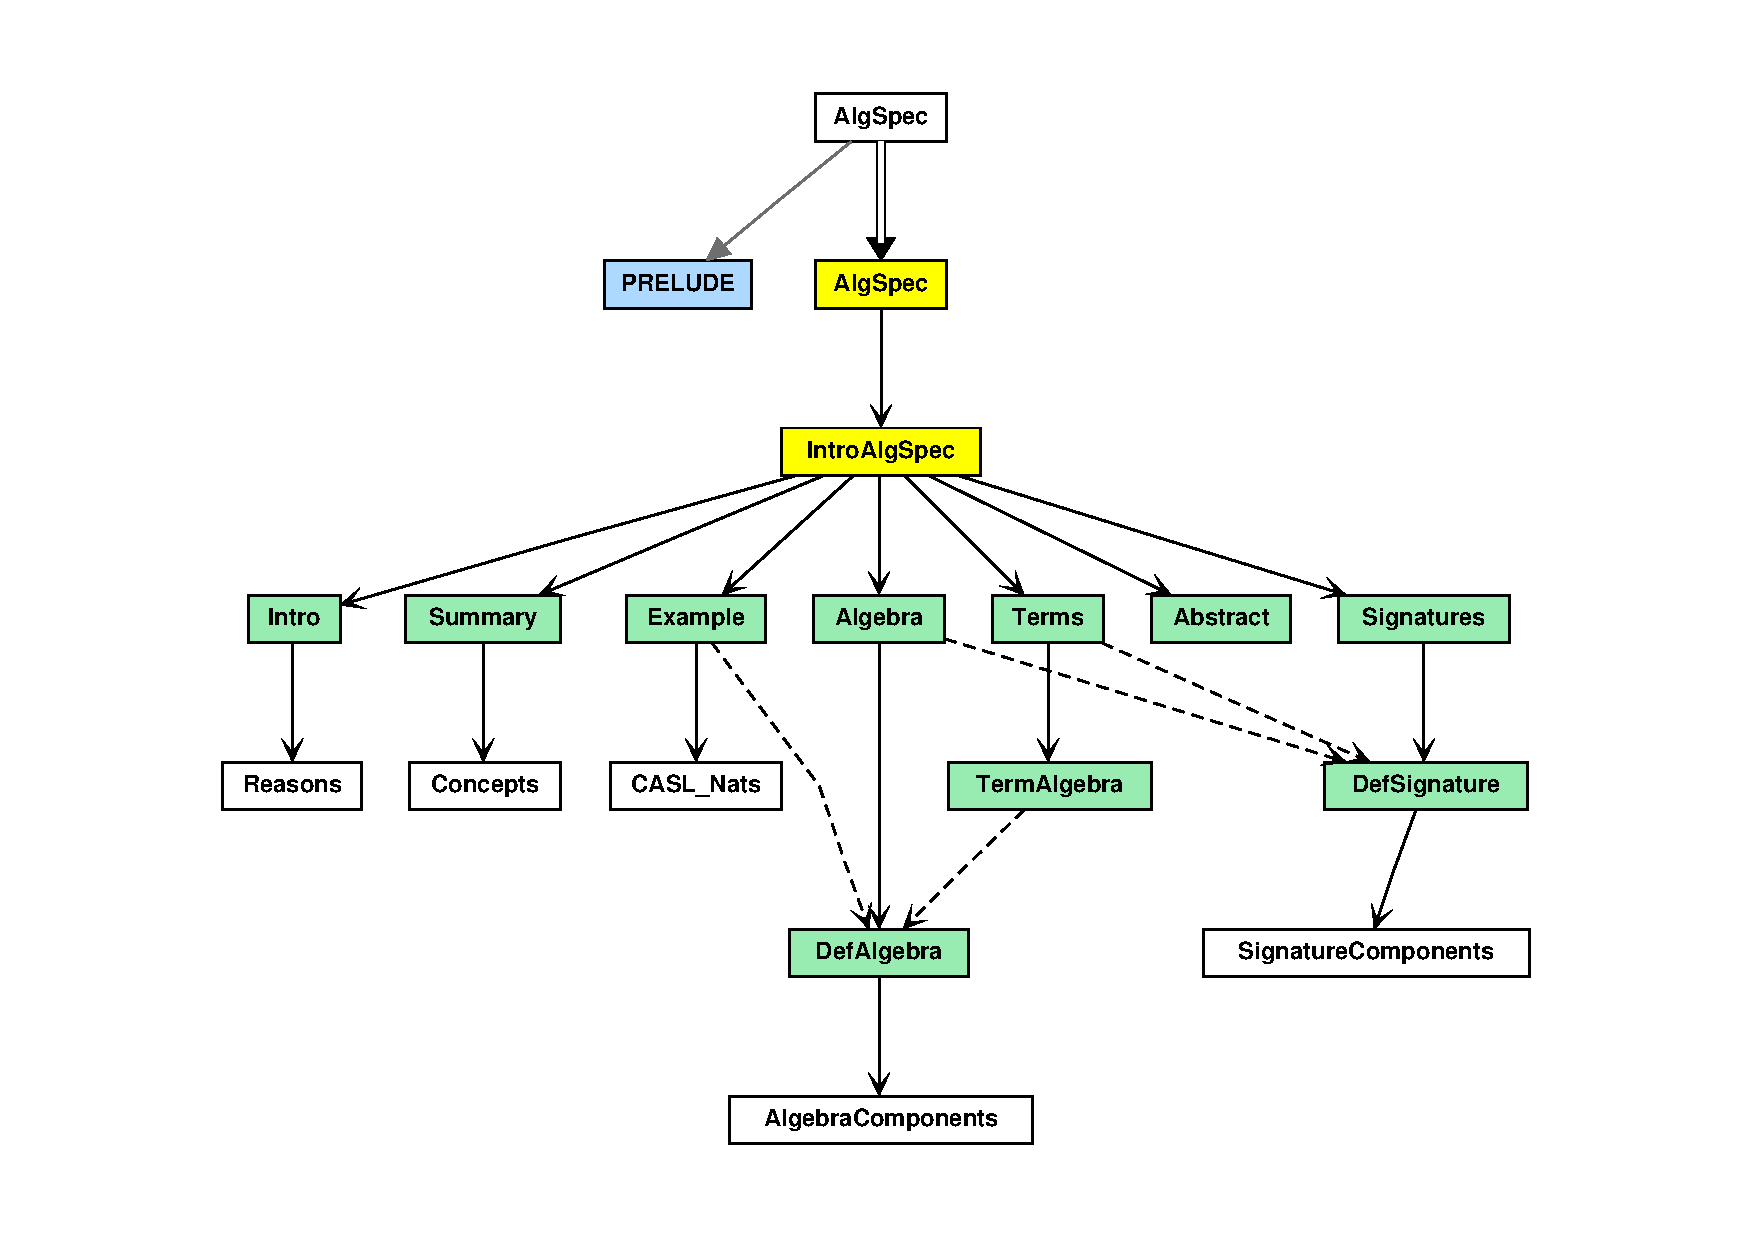
\includegraphics[width=\textwidth]{img/example-doc-graph}
    \caption{Structure Graph of Example Document.}
    \label{fig:example-doc-graph}
  \end{center}
\end{figure}
\end{Paragraph}
\end{Section}
\end{Section}

\begin{Section}[Title={Representation and Exchange Formats},Label={Representation_and_Exchange_Formats}]
\begin{Paragraph}
%\subsection{Representation and Exchange Formats}
\end{Paragraph}

\begin{Section}[Title={MMiSS-XML},Label=s37]
\begin{Paragraph}
%\subsubsection{MMiSS-XML}
The principal representation and \ExternalExchangeFormat{} for documents in the \Repository{} is
\DefClass{MMiSSXML}{\MMiSSXML}, 
a straightforward translation of the document \DocStructuringOperation{}s
introduced in Sect.~\ref{Sec-SemanticDocumentStructuring}
into \XML{}. However, \XML{} is not meant to be read or written by human
users, and tools have their own input formats, hence for presentation
and editing purposes, we need external exchange formats. 
An 
\DefClass{ExternalExchangeFormat}{\ExternalExchangeFormat}
is incorporated into \MMiSS{} by implementing a
structure parser, which converts documents in the \ExternalExchangeFormat{} into
\MMiSSXML{} and back. Presently, this has been implemented for a \LaTeX{} dialect
called 
{\MMiSSLaTeX}, 
and is in preparation for
\OMDoc{} \cite{+++++}. 
More external exchange formats will be added if and when
editing and presentation tools accepting and requiring these formats
will be incorporated into the \MMiSS{} system.

\MMiSSXML{} is a straightforward translation of the
\DocStructuringOperation{}s introduced in
Sect.~\ref{Sec-SemanticDocumentStructuring} into the extensible
markup language \XML{}. There are elements corresponding to the groups,
units and atoms. \MMiSSXML{} is fairly verbose, and not intended for
user interaction
before suitable wysiwyg editors become available. 

Recall that in \XML{}, documents are represented by attributed trees,
which are typed by \emph{\XMLDocTypeDef{}s} 
({\DTD}s)\footnote{Or  schemas, but we're old skool here.}. 
A \DTD{} gives the production
rules for the \XMLDocTypeDef{}s (the \Node{}s of the tree), and the
admissible \XMLAttribute{}s for each element. 

To illustrate this concept, we will follow our example document above
round the system architecture, as it is retrieved from the \Repository{},
converted into {\MMiSSLaTeX} 
and presented to the user. We focus on the
definition of an algebra (labelled \Algebra{} in
Fig.~\ref{fig:example-doc-graph}). This \GroupStr{} is a \ParagraphStr{},
containing an introductory sentence, and a \DefinitionStr{} labelled
%$\Sigma$-Algebra
\GivenName{DefAlgebra}{}. The \DefinitionStr{}  contains a list enumerating the
components of a 
\SigmaAlgebra{}.
As it is retrieved from the
\Repository{}, the document is in \MMiSSXML{} format.
\end{Paragraph}
\end{Section}

\begin{Section}[Title={MMiSSXML Example},Label={MMiSSXML_Example}]
\begin{Paragraph}
%\subsubsection{MMiSSXML Example}

\BKB{neu (s.o.) bzw. evtl. k\"urzen, besonders die Beispiele}

Here is an excerpt of the relevant part of the \MMiSSXML{} \DTD{}.
First, the following \Emphasis{\XMLEntityDef{}s}  (essentially, macro
definitions) define a unit to be either a conceptual or formal unit,
or an atom, which in turn is either a conceptual or formal atom. (We
have omitted the lengthy definition of atoms.)
\begin{Source}
<!ENTITY % conceptualUnit  "example | exercise | definition" >

<!ENTITY % formalUnit  "program | theory | theorem | conjecture | lemma 
                        | corollary | assertion | development | proof 
                        | script" >

<!ENTITY % unit   "%conceptualUnit; | %formalUnit; | %atom; ">
\end{Source}

The following \emph{\XMLElementDef{}s} define the actual elements. A
\ParagraphStr{} contains a sequence of units and can have all the usual
attributes. It is visualised by a yellow box, as specified by the
\DefClass{MMiSSDisplay}{\MMiSSDisplay}
directive. Analogously, a definition 
(a green box) contains a
sequence of units: 
\begin{Source}
<!ELEMENT paragraph (%unit;)+>
<!ATTLIST paragraph %attributes;>
<?MMiSSDisplay paragraph : yellow box ?>

<!ELEMENT definition (%unit;)+>
<!ATTLIST definition %attributes;>
<?MMiSSDisplay definition : Green box ?>
\end{Source}
For each of the \StructuralEntities{} from
Sec.~\ref{Sec-SemanticDocumentStructuring} there is a corresponding
\XMLElementDef{}. The structural \Attribute{}s are modelled by 
\XML{}-\XMLAttribute{}s; a very brief excerpt shows the definition of structure
attributes:

\begin{Source}
<!ENTITY % structure-attr "label        CDATA  #IMPLIED
                           title        CDATA  #IMPLIED
                           formalisms   CDATA  #IMPLIED">

<!ENTITY % attributes "%structure-attr;
                       %version-attr; 
                       %variant-attr; ">
\end{Source}
With this \DTD{}, the definition of an algebra looks as follows in
\MMiSSXML{}:

\begin{Source}
<paragraph label="Algebra" title="Algebra">
<textFragment><![CDATA[Algebras are models of ]]>
<link linked="DefSignature" status="present"><![CDATA[signatures]]>
</link>
<![CDATA[.]]>
</textFragment>
<definition label="DefAlgebra" title="$\Sigma$-Algebra">
<list label="AlgebraComponents" listType="itemize">
<listItem>
  <textFragment>
    <![CDATA[for each sort $s \in S$, a ]]> 
    <emphasis><![CDATA[carrier set]]><\emphasis>
    <![CDATA[$A_s \in S_A$;]]>
  </textFragment>
<listItem>
  <textFragment>
    <![CDATA[for each operation $\omega:s_1\ldots s_n \rightarrow s$, 
             an operation $\omega_A:A_{s1}\ldots A_{sn} \rightarrow A_s$]]>
  </textFragment>
</list>
</definition>
</paragraph>  
\end{Source}
This definition is in fact produced by the structure parser from a
corresponding {\MMiSSLaTeX} input. 
The structure parse will also
reconstruct the {\MMiSSLaTeX} 
code from the \MMiSSXML{} document when it
is checked out from the \Repository{}. 

\end{Paragraph}
\end{Section}
\begin{Section}[Title={MMiSSLaTeX},Label={MMiSSLaTeX}]
\begin{Paragraph}
%\subsubsection{MMiSSLaTeX}

\begin{figure}[htbp]
  \begin{center}
    \includegraphics[width=\textwidth]{img/rep-alg-slide}
    \caption{Example Slide: Definition of an Algebra.}
    \label{fig:rep-alg-slide}
  \end{center}
% \BKB{nur wenn ich diesen Kommentar einfuege erscheint diese Fig NICHT auf einer eigenen Seite? wieso?}
\end{figure}

\DefClass{MMiSSLaTeX}{\MMiSSLaTeX}
is the authoring language for \MMiSSXML{},
a \LaTeX{} style (essentially, a class file)
providing \LaTeX{} \LaTeXCommand{}s for each of the structuring
operations from Sec.~\ref{Sec-SemanticDocumentStructuring}. 
Most of
these are defined as \LaTeXEnvironment{}s, e.g.
for paragraphs, definitions, lists and so on. The attributes are given
as optional arguments to the  \LaTeXEnvironment{}s or  \LaTeXCommand{}s.
Here is the  definition of an algebra in \MMiSSLaTeX{}:
\begin{Source}
\\begin{Paragraph}[Label=Algebra, Title=Algebra]
Algebras are models of \Link[LinkText=signature]{DefSignature}.
\begin{Definition}[Label=DefAlgebra, Title={$\Sigma$-Algebra}]
  An \Emphasis{Algebra} $A= (S_A, \Omega_A)$ for a signature
  $\Sigma=(S, \Omega)$ ($\Sigma$-Algebra) is given by 
  \begin{List}[Label=AlgebraComponents, ListType=itemize]
    \ListItem for each sort $s\in S$, a \Emphasis{carrier set} $A_s\in
    S_A$; \ListItem for each operation $\omega:s_1\ldots
    s_n\rightarrow s$, an operation $\omega_A:A_{s1}\ldots
    A_{sn}\rightarrow A_s$.
  \end{List}
\end{Definition}
\end{Source}

The document is edited in \MMiSSLaTeX{}, and it is typeset using
normal \LaTeX{} with the \MMiSSLaTeX{} class file. The class file
translates e.g. a \SourceText{List} \LaTeXEnvironment{} into \LaTeX'
\SourceText{itemize} \LaTeXEnvironment{}. The resulting slide is shown in
Fig.~\ref{fig:rep-alg-slide}.
%Note that above we only show a brief excerpt of the \MMiSSLaTeX{}
%code. Hence, most of the attributes are not actually shown (such as
%Author, Language, Formalism etc.) since they are inherited.
\end{Paragraph}
\end{Section}
\end{Section}

\begin{Section}[Title={Authoring Tools},Label={Authoring_Tools}]
\begin{Paragraph}
%\subsection{Authoring Tools}

%% following subsection was commented out allready
% %\subsubsection{User Interfaces}
\label{sec:user-interfaces}

\BKB{CXL: evtl. mit  \MMiSSLaTeX{} (s.o.) zusammen fassen; \TextEditor{} und \GraphEditor{} ergaenzen}

%% siehe oben:
%The \GraphEditor{}, i.e. the user interface to the \DevelopmentManager{}, 
%and the \TextEditor{} constitute the major \AuthoringTool{}s.


Users interacting with the {\DevelopmentManager} and  \Repository{} are either \AuthorRole{}s
editing documents, or \StudentRole{}s to whom documents are presented in
learning situation. As we can see from Fig.~\ref{fig:repository-sysarch},
these two r\^oles correspond to different user interfaces.

A student is presented
with a \PDF{}, \PS{} or \HTML{} document via the typical 
\PresentationPlatform{}s (a \PDF{} reader, a \PS{} printer, or an \HTML{} browser).


For authors, there are two interfaces through which they interact with
the \Repository{}. Firstly, the documents in the \Repository{}
form a \StructureGraph{}, augmented by different {\Version}s to a
{\DevelopmentGraph}; these are
navigated with the \GraphVisualisation{} and browsing tool daVinci.
\BKB{davinci ref}
Secondly, documents can be edited in the \MMiSSLaTeX{} exchange format
with an \XEmacsEditor{}, using a particular \MMiSSLaTeX{} mode. In
both cases, the predominant interaction paradigm is 
\Emphasis{direct manipulation} 
--- authors do not have to learn cryptic command lines
to interact with the \Repository{}, they essentially just point at the
\RepositoryObject{} of interest, and/or select from a menu of given choices.

The \RepositoryObject{}s in the \Repository{} are organised in folders, which allow
the grouping of \RepositoryObject{}s much like directories in a file system.
Folders may contain other folders, or \MMiSS{} \StructuralEntities{}, i.e. groups,
units or atoms.  
%The \emph{object graph} contains the folders and objects
The \StructureGraph{} contains the hierarchy of folders and, 
at the leaves of this hierarchy, the  
structure of the \RepositoryObject{}s  inside a \PackageStr{}, as \Node{}s, 
with \Edge{}s corresponding to the \Contains{}{}{} relation (resulting from nesting and
\StructuralSharing{}), as shown in
Fig.~\ref{fig:repository-versiongraph}. 
In the \StructureGraph{}, the user can select a \Node{}, corresponding to an
\RepositoryObject{}, to edit in one of the external exchange formats. (Presently,
the only viable option here is \MMiSSLaTeX{}, since \MMiSSXML{} is not
meant for user interaction.) 
In the case of \MMiSSLaTeX{}, the
%\MMiSSLaTeX{} 
code is loaded into an \XEmacsEditor{} (which is driven
from the {\DevelopmentManager} ), 
and the user can edit it there.
A special
\MMiSSLaTeX{} mode, inspired by the \AUCTeX{} mode, gives the user
\BKB{CXL: AUCTEX ref}
additional editing assistance, e.g.  to insert \LaTeXEnvironment{}s or
\LaTeXCommand{}s.

\begin{figure}[htbp]
  \begin{center}
    \includegraphics[width=\textwidth]{img/repository-objectgraph}
  \end{center}
  \caption{The Structure Graph: Editing the Definition of a \SigmaAlgebra}
  \label{fig:repository-objectgraph}
\end{figure}

Since \StructuralEntities{}  can get quite large (for example, a whole
\PackageStr{}), we only display one level in the \XEmacsEditor{}; nested \StructuralEntities{} 
are displayed by clicking buttons. For example,
Fig.~\ref{fig:repository-objectgraph} shows  
the \ParagraphStr{} labelled \GivenName{Algebra} being edited. It contains the definition
labelled \GivenName{DefAlgebra}, which has been opened, and the user is
just about to open the list \GivenName{AlgebraComponents}.
\end{Paragraph}
\begin{Section}[Title={Implementation Issues},Label={Implementation_Issues}]
\begin{Paragraph}
%\subsubsection{Implementation Issues}

\CXL{Could go to the end of this section.}
\BKB{oder nach oben? wohin?}
The \Repository{} is implemented almost entirely in the functional
programming language \Haskell{} in about 60 Kloc. The \Repository{} uses the
open source data base BerkeleyDB \cite{BerkeleyDB} to store documents.
The graph visualisation system daVinci, the graphical user interface
library Tcl/Tk \cite{Ousterhout} and the \XEmacsEditor{} are encapsulated in
\Haskell{}.  These encapsulations are available separately, and can be
used independently, in particular the Tk encapsulation, called HTk.
\BKB{CXL: refs for HTk}

The content model is generic over the \XML{} \DTD{} used (although of course
the structure parsers for the external exchange formats are not),
so the \Repository{} can be used for other document formats as well. More
importantly, small changes in the \DTD{} can be implemented directly
without needing to recompile the \Repository{}. To parse the \DTD{} and the
documents, we use the Haskell \XML{} library HaXML \cite{HaXML}. 
\end{Paragraph}
\end{Section}
\end{Section}

\begin{Section}[Title={The Development Manager},Label={The_Development_Manager}]
\begin{Paragraph}
%\subsection{The Development Manager}
\end{Paragraph}
\begin{Section}[Title={Version Control and Configuration Management},Label={Version_Control_and_Configuration_Management}]
\begin{Paragraph}
%\subsubsection{Version Control and Configuration Management}
\label{sec:version-control}

The art of keeping track of the evolution
of complex systems in general, and complex documents in this case,
is implied in the notion of
\DefClass{ConfigurationManagement}{\ConfigurationManagement}.
This means that changes to a documents are organised and recorded,
such that we can always return to an earlier configuration. Usually,
configuration \RepositoryObject{}s are source files, but here we follow a
\Emphasis{fine-grained} approach, where our configuration \RepositoryObject{}s are the
\StructuralEntities{} of the \MMiSS{} document structure, i.e. \GroupStr{}s, \UnitStr{}s
or \AtomStr{}s and associated \Attribute{}s. 

\begin{figure}[htbp]
  \begin{center}
    \includegraphics[width=.5\textwidth]{img/repository-versiongraph}
    \caption{A Version Graph displayed by daVinci}
    \label{fig:repository-versiongraph}
  \end{center}
\end{figure}
\end{Paragraph}
\end{Section}

\begin{Section}[Title={Version Graph},Label={Version_Graph}]
\begin{Paragraph}
%\subsubsection{Version Graph}
The 
\DefClass{VersionGraph}{\VersionGraph} is the representation underlying
\DefClass{VersionControl}{\VersionControl}; 
it has as \Node{}s the different
\DefClass{Version}{\Version}s 
 of the
\RepositoryObject{}s, and as \Edge{}s the 
\DefClass{RevisionOfRelation}{\RevisionOfRelation}. 
An author always starts interaction with the \Repository{} from the
\VersionGraph{}, picking a \Version{} to start working on.
Fig.~\ref{fig:repository-versiongraph} shows a typical \VersionGraph{}, as
displayed by daVinci. From the \VersionGraph{}, a particular \Version{} to
work on is selected by double-click to  
\DefClass{CheckOut}{\CheckOut} 
this \Version{} into the user's local filespace. It can then be edited in the \VersionGraph{}. 
In Fig.~\ref{fig:repository-versiongraph}, version~2.0 is the current
\DefClass{WorkingVersion}{\WorkingVersion} 
(as visualised by the red circle). After
editing the \RepositoryObject{}, users may 
\DefClass{Commit}{\Commit} 
changes back into the
\Repository{} (or they may just dispose of them silently). A new \Version{} 
of the changed \RepositoryObject{} is created, and of all \RepositoryObject{}s containing the
changed \RepositoryObject{}. 
\BKB{CXL: wie weit? bis zum package?}
Thus, new \Version{}s propagate upwards: a change in a
constituting \RepositoryObject{} results in a new \Version{}  of the parent \RepositoryObject{}.


\BKB{CXL: was genau ist der Development Graph?Combination of Structure and Version Graph?!}
\BKB{CXL: erlaeutern}
%               \DeclClass{WorkingVersion}{working version}{Version}{\WorkingVersion}
%               \DeclClass{CompatibleVersion}{compatible version}{Version}{\CompatibleVersion}
\end{Paragraph}
\end{Section}

\begin{Section}[Title={Revision Operations},Label={Revision_Operations}]
\begin{Paragraph}
%\subsubsection{Revision Operations}
\BKB{BKB, cxl: ergaenzen}
%               \DeclClass{Revision}{revision}{Version}{\Revision}
%               \DeclClass{Extension}{extension}{Version}{\Extension}
%               \DeclClass{ConservativeExtension}{conservative extension}{Version}{\ConservativeExtension}
\end{Paragraph}
\end{Section}

\begin{Section}[Title={Merging},Label={Merging}]
\begin{Paragraph}
%\subsubsection{Merging}
\BKB{CXL, AM: ergaenzen}
\end{Paragraph}
\end{Section}
\end{Section}

\begin{Section}[Title={Change Management},Label={Change_Management}]
\begin{Paragraph}
%\subsection{Change Management}
\label{sec:change-management}
\RevisedBy{BKB 030424}

The notion
\DefClass{ChangeManagement}{\ChangeManagement} 
 is used for the maintenance and preservation of \ConsistencyConf{} and \CompletenessConf{} of a development during its evolution.
More precisely, we want to have a \DefClass{ConsistentConfiguration}{\ConsistentConfiguration} in which all constituents harmonise, \Version{}s are compatible, \ReferenceStr{}s and \LinkStr{}s refer to the proper targets, etc.
At the same time, it should be a \DefClass{CompleteConfiguration}{\CompleteConfiguration}: e.g. the promises of forward \ReferenceStr{}s and \LinkStr{}s should be fulfilled, i.e. they must not be dangling; if we have an English and a German \Variant{} of a whole document, then we expect to have a corresponding German \Variant{} for each English \Variant{} for all constituent StructuralEntities{}, with the same overall structure and relations, and vice-versa.

Such notions are well-known for formal languages; in contrast, natural language used for writing teaching material does not usually
possess a well-defined semantics; the notion of consistency is debatable. 
Different authors may postulate different requirements on the material in order to regard it as being
consistent.
The existence of an \Ontology{} already helps  a great deal to check \ReferenceStr{}s .

It turns out that the notions of \ConsistencyConf{} and \CompletenessConf{} 
are closely related to the \DocStructuringOperation{}s and \DocRelation{}s.
Below we will discuss some of these and elaborate on emerging properties and their interaction
in order to illustrate the variety of requirements authors may postulate.

\begin{description}
\item [Contains]
An obvious structuring mechanism is nesting of individual parts of a document, leading to the \Contains{}{}{} relation. 
%Its Inverse is the ContentOf{} relation.
A \ParagraphStr{} is contained in a
{\SectionStr}, while {\SectionStr}s are themselves contained in \PackageStr{}s. \MMiSS{} defines a hierarchy of 
\StructuralEntities{} to define the \Contains{}{}{} relation, e.g. \PackageStr{}s, {\SectionStr}s, {\UnitStr}s, or {\AtomStr}s, see Sec.~\ref{sec:document-structure}.

\item [ReliesOn, PointsTo]
Besides the \Contains{}{}{} relation, there is a family of \DefClass{ReliesOnRelation}{\ReliesOnRelation}s, reflecting the various dependencies between different parts of a document. 
For example, a \TheoremStr{} \DefRelation{LivesIn}{\LivesIn} a {\TheoryStr}, 
a \ProofStr{} \DefRelation{Proves}{\Proves} a {\TheoremStr}, 
an \ExampleStr{} \DefRelation{Illustrates}{\Illustrates} a {\DefinitionStr}, 
and so on. In this case, we would usually like to insist on a linear \Order{} of appearance, i.e. the right-hand-side    (target) of the relation should (textually) be presented before the left-hand-side.
The family of \DefClass{PointsToRelation}{\PointsToRelation}s is very similar, but we may tolerate forward pointers: 
a \ReferenceStr{} \DefRelation{References}{\References} a {\DefineElementStr} occurrence, similarly for \LinkStr{}s,
a \CitationStr{} \Cites{}{}{} a \BibEntryStr{},  and so on. 

%       Introducing a terminology with the help of definitions (cf ???) the latter use of this terminology
%       depends on its introduction. 

\item [VariantOf]
Another structuring \DocRelation{} is introduced by the various notions of \Variant{}s. Parts of a document may e.g. be written in various languages which gives rise to a \DefClass{VariantOfRelation}{\VariantOfRelation} between these document parts and their constituents.
%       MMISS provides different forms of documents, like slides, scripts, book etc, which operate on
%       different levels of detail. Slides are less detailed than scripts or books. Furthermore, there may be
%       different ways to axiomatize or specify a given learning material. Different \Version{}s of the same material
%       may be exchangable.
\BKB{AM: more?}

\end{description}


For special \FormalismAttribute{}s, additional structuring \DocRelation{}s
may be explored by special tools operating on these. \CASL{}, for instance, offers the notions of extension, union, etc., to define dependencies between specifications.

The \ChangeManagement{} keeps track of the various structuring mechanisms described above. Below we will tentatively explore various properties of the individual structuring mechanisms to illustrate 
possible notions of \ConsistencyConf{} and \CompletenessConf{} and their interaction. 
Postulating such invariant properties as 
requirements on the \ConsistencyConf{} and \CompletenessConf{}  of a document, and formulating these invariants as formal rules,
will enable us to implement a generic and flexible \ChangeManagement{} that keeps track of the various invariants and
informs the user about violations when a previously consistent document has been revised.
\end{Paragraph}
\begin{Section}[Title={Properties of individual structuring mechanisms},Label={Properties_of_individual_structuring_mechanisms}]
\begin{Paragraph}
%\subsubsection{Properties of individual structuring mechanisms}

For each of the structuring mechanism described above we can formulate various invariants that
are prerequisites for  \ConsistencyConf{} or \CompletenessConf{} . Some of these are enforced by the underlying structuring language (\MMiSSLaTeX{}) but others may be violated once the user revises a document.

\begin{description}
\item[Contains]
Obviously the \Contains{}{}{} relation is reflexive, transitive and antisymmetric denoting
an acyclic finite graph (which is actually a subgraph of the \StructureGraph{}). These properties are 
trivially enforced by the \DocStructuringOperation{}s. We may want to require additional invariants for \ConsistencyConf{}, e.g. that
each of the major \StructuralEntities{} (such as \PackageStr{}, {\SectionStr}, or {\ParagraphStr}) contains at least one \UnitStr{} or \AtomStr{}, or that there is at most one \SummaryStr{} in a \SectionStr{}. 
%       Regarding other, embedded
%       formal languages in MMISS we adopt their corresponding ``\Contains{}{}{} relations'' of these languages. 
%       E.g. a body of while loop is content of the while loop, 
%       or \AxiomStr{}s are content of a formal \TheoryStr{} in CASL.

\item[ReliesOn, PointsTo]
Each \ReliesOnRelation{} or \PointsToRelation{} is irreflexive and acyclic. We would also postulate as a \ConsistencyConf{} requirement that there is at most one target, i.e. the relations are in fact many-to-one; a \CompletenessConf{} requirement is that that there is at least one target, e.g. \ReferenceStr{}s must not be dangling; both together require a unique target. 
Furthermore, we require the target to be presented beforehand.
However, the \CompletenessConf{} requirement may be weaker for \PointsToRelation{}s as we tolerate forward pointers, even to other, future \PackageStr{}s (warnings should be given, though).

Regarding special  \FormalismAttribute{}s, we adopt their \ReliesOnRelation{}s and corresponding properties. \AxiomStr{}s in \CASL{}, for instance, depend on their global environment resulting from fragments of the reps. \TheoryStr{} that specifies the signature of the symbols used in the \AxiomStr{}s.

\item[VariantOf]
The semantics of the \VariantOfRelation{}s depends on the various types of \Variant{}s. Regarding \Variant{}s in different languages (or on different levels of detail), we impose the \CompletenessConf{} requirement that each \Variant{} in one language must have a corresponding \Variant{} in the other, for all constituent \StructuralEntities{}, with the same overall structure and relations (as an option, for each level of detail, and so on).
Similarily one will be able to specify, as a  \ConsistencyConf{} requirement, that all \ProgramStr{}s should be in a particular \FormalismAttribute{}, e.g. the programming language \Haskell{}. 
A corresponding \CompletenessConf{} requirement would be that we have, for each \ProgramStr{}, a \Variant{} in programming language \C{} and \JAVA{}, e.g. for different \TeacherRole{}s of a course. 

\end{description}
\end{Paragraph}
\end{Section}

\begin{Section}[Title={Properties of Interactions between Structuring Mechanisms},Label={Properties_of_Interactions_between_Structuring_Mechanisms}]
\begin{Paragraph}
%\subsubsection{Properties of Interactions between Structuring Mechanisms}

While the properties mentioned above are specific to an individual structuring mechanism, we will
explore possible interactions of different structuring mechanisms and how they can be used to
refine \ConsistencyConf{} and \CompletenessConf{}.

\begin{description}
\item[Contains{} vs. ReliesOn]
Relating the \Contains{}{}{} and \ReliesOnRelation{}s (we subsume \PointsToRelation{}s here)  allows us to formalize constraints regarding the closure of document
parts with respect to the \ReliesOnRelation{}. We may require, for example, that
%       all citations refer to bibliography entries of the same \PackageStr{} 
there is a \ProofStr{} for each {\TheoremStr} in a \PackageStr{} or that  
each \ReferenceStr{} \References{}{}{} a {\DefineElementStr} occurrence in this \PackageStr{} unless there is an explicit import.
Furthermore, a  \ReliesOnRelation{} between two \StructuralEntities{} is propagated along
the \Contains{}{}{} relation towards the root of the hierarchy of nested \StructuralEntities{}. 
Consider, for example, a \ProofStr{} in \SectionStr{} A that \Proves{}{}{} a {\TheoremStr} in \SectionStr{} B, then \SectionStr{} A \ReliesOn{}{}{} \SectionStr{} B.
Conversely, a  \ReliesOnRelation{} between two \StructuralEntities{} cannot be decomposed and propagated towards the leaves. 
Changing (parts of) one of them can affect the proposed  \ReliesOnRelation{}. 
%       In this case it is up to the user to declare for instance the changes as a
%        conservative extension of the old one.

\item[Contains{} vs. VariantOf]
The interaction between the \Contains{}{}{} and the \VariantOfRelation{} is rather subtle and has not fully been investigated yet. For example, we expect the structure of a document with the \LevelOfDetailAttribute{} \LectureAttribute{} to be a homomorphic projection of the corresponding structure with the \LevelOfDetailAttribute{} \CourseAttribute{}.
%       Z.B. alle sprachvarianten haben gleiche strukturierung (wird y.B. in ActiveMath durch die
%       Syntax automatisch erzwungen)

\item[ReliesOn vs. VariantOf]
Similarly, the interaction between the \ReliesOnRelation{} (or \PointsToRelation{}) and the \VariantOfRelation{} merits further investigation. It is not clear what kind of relations  across \Variant{}s are desired, if any. In principle, each \Variant{} should be closed with respect to \ReliesOnRelation{}s, i.e. all targets should be provided in that \Variant{}. An exception might be an explicit pointer to material in a \LectureDoc{} from a \CourseDoc{}, but then this material should be included in the \CourseDoc{} anyway as a \CompletenessConf{} requirement. The converse is more likely: one might want to make a pointer into a more detailed \CourseDoc{} or \LectureNotesDoc{} document from slides in a \LectureDoc{}. 

\end{description}

In any case, the more structure there is, the better are the chances for preserving \ConsistencyConf{} and \CompletenessConf{}; any investment in introducing more \ReliesOnRelation{}s, for example, will pay off eventually.
The \ChangeManagement{}  will observe whether revisions by the user will affect these relations
and, depending on the user's preferences, emit corresponding warnings. It is crucial to point out that, 
in contrast to formal developments such as in the MAYA-system \cite{},
\BKB{DH: citation}
there is no rigorous requirement that a document should obey all the rules mentioned above. There may be good reasons, for instance, to present first a ``light-weight'' introduction to all notions introduced in a \SectionStr{} before giving the detailed definitions. In this particular case, one would want to introduce forward pointers to the definitions rather than making the definitions rely on the introduction; thus the rules are covered. 

\BKB{DH: ueberarbeiten oder streichen}
Zielsetzung ist, dass der Benutzer selbst die Kriterien, welche von dem System ueberprueft werden
soll. Diese spalten sich along the different structuring mechanisms into the following categories:
rules to control 
\begin{itemize}
\item the overall document structure (\Contains{}{}{}  relation), 
\item the semantic relation 
\item aspects of various variants
\item dependencies between \Contains{}{}{}  and semantic relation
\item dependencies between \Contains{}{}{}  and \VariantOfRelation{}
\item dependencies between \Contains{}{}{}  and \VariantOfRelation{}
\end{itemize}

\BKB{DH: siehe auch neue Ergaenzung in Architecture: Integration of Foreign Tools; besser hier?}
\end{Paragraph}
\end{Section}
\end{Section}


%%%%%%%%%%%%%%%%%%%%%%%%%%%%%%%%%%%%%%%%%
\end{Section}
\end{Section}

%\subsection{Tools for Interaction and Administration}
\begin{Section}[Title={Tools for Interaction and Administration},Label={Tools_for_Interaction_and_Administration}]
\begin{Paragraph}
\BKB{der Abschnitt haengt etwas in der Luft, aber wohl am besten hier}
\end{Paragraph}
\begin{Section}[Title={Integration of Foreign Tools},Label={Integration_of_Foreign_Tools}]
\begin{Paragraph}
%\subsubsection{Integration of Foreign Tools}
\BKB{DH: ergaenzen; hier?}
BKB {DH: ergaenzen}
\end{Paragraph}
\end{Section}

\begin{Section}[Title={WebAssign},Authors={A. Poetzsch-Heffter},Label=s52]
\begin{Paragraph}
%\subsubsection{WebAssign}
%\Authors{A. Poetzsch-Heffter}
The \WebAssign{} system developed at FernUniversit\"at
Hagen 
(see \cite{WebAssignArticle} or http://niobe.fernuni-hagen.de/WebAssign)
supports web-based distribution, correction, and
administration of course related assignments. Assignments
may have interactive parts where system gives
direct feedback to the student. \WebAssign{} also manages
the integration of external tools (such as compilers) that
check student answers or provide help in other ways.
In addition, \WebAssign{} provides a flexible administrative support.
The \WebAssign{} subsystem is presently being integrated.
\BKB{APH: klappt die Integration von WebAssign noch?}
\end{Paragraph}
\end{Section}
\begin{Section}[Title={User Management},Authors={A. Poetzsch-Heffter},Label=s53]
\begin{Paragraph}
%\subsubsection{User Management}
%\Authors{A. Poetzsch-Heffter}
A \UserManagement{} component supports a simple user
model with different \Role{}s and handles the access
rights of \AuthorRole{}s, \TeacherRole{}s,  \StudentRole{}s, \TutorRole{}s, \CorrectorRole{}s, 
and also \ToolDeveloperRole{}s, \SystemDeveloperRole{}s, and \AdministratorRole{}s.
BKB: {APH: mehr zur Nutzerverwaltung? rollenbasierte Zugriffskontrolle?}
BKB: {APH: im aelteren Papier (auch auf meinen Folien) war immer ausfuehrlich was zu den Rollen gesagt. Ueberarbeitest Du das nochmal? am Anfang bei den Zielen? oder reicht das? s. Ontology}
%       The relation between the architectural components and
%       the goals explained at the beginning of this abstract is
%       shown at the right side of the diagram.
\end{Paragraph}
\end{Section}
\begin{Section}[Title={Installation Package},Authors={},Label=s54]
\begin{Paragraph}
\subsubsection{Installation Package}
\BKB{APH, DH: etwas dazu?}
BKB {APH, DH: etwas dazu?}
Dieter: Die Diskussion in Warschau zeigt uebrigens, dass der Broker, wenn er denn auch zum Bootstrap genutzt werden soll,  m.E. nicht in Mozart sondern einer Sprache mit erzeugbarem Binary geschrieben werden sollte (C, Java, Haskell); Mozart wird ohnehin sonst nur in Spezialfaellen gebraucht.
\end{Paragraph}
\end{Section}
\end{Section}
\end{Section}

% Presentation
\begin{Section}[Title={Presentation},Label={Presentation}]
\begin{Paragraph}
%\input{presentation.tex}
%\section{Presentation}
\label{sec:presentation}
\RevisedBy{BKB 030426 and again JGS 030507}


%       As became clear in the previous sections, the aim of the \MMiSS{} project
%       is to produce teaching content in the field of Safe and Secure
%       Systems, which can be presented in many different forms using
%       various media. 

%It is a good idea in general to separate issues of \Emphasis\Presentation{} 
%from a \Emphasis{re}presentation in an abstract form (\MMiSSXML{} here) 
%that can also serve as an \ExternalExchangeFormat{}, and authoring languages 
%(such as \MMiSSLaTeX{}).

%This section concentrates first on \Presentation{} issues such as \Layout{} and \Animation{},
%and how they can be treated in \MMiSSLaTeX{}. 
%Work is under way to isolate and separate these as attributes 
%to relieve an \AuthorRole{} from tedious formatting as much as possible.
%Ideally, tools will generate different presentation forms automatically.
%The subsystem \ActiveMath{}, which is developed separately, 
%is integrated via a mapping from \MMiSSXML{} to \OMDoc{}
%and provides user-adaptive presentation based on pedagogic rules.

In this section, we concentrate on \Presentation{} issues such as
\Layout{} and \Animation{}, and show how they can be realised using
the authoring language \MMiSSLaTeX{}.

In general, \Emphasis{\Presentation{}} issues should be separated
from issues of \Emphasis{re}presentation in an abstract form
(\MMiSSXML{} here), which can also serve as an
\ExternalExchangeFormat{}. In fact, the \AuthorRole{} should be
relieved from tedious formatting as much as possible. Therefore, work
is under way to isolate layout and animation as attributes.   
Ideally, tools will generate different presentation forms automatically.
The subsystem \ActiveMath{}, which is developed separately, 
is integrated via a mapping from \MMiSSXML{} to \OMDoc{}
and provides user-adaptive presentation based on pedagogic rules.
\end{Paragraph}
\begin{Section}[Title={Layout in MMiSSLaTeX},Label={Layout_in_MMiSSLaTeX}]
\begin{Paragraph}
%\subsection{Layout in MMiSSLaTeX}
\label{Layout-MMiSSLaTeX}

\end{Paragraph}
\begin{Section}[Title={Annotating Slides},Label={Annotating_Slides}]
\begin{Paragraph}
%\subsubsection{Annotating Slides}
\Authors{Jan-Georg Smaus} 
\RevisedBy{BKB 030426 and again JGS 030507}

\BKB{ArneL: ergaenzen}

At Universit{\"a}t Freiburg, experiments have been made to enhance slides 
for the course \Emphasis{Computer-Supported Modelling and Reasoning}
(held regularly each year) towards a self-contained online course.
We will report on our experiences below; 
they have led to new insights into the best ways of defining the 
\Layout{} (and \Animation{}) of the
\LevelOfDetailAttribute{}  \LectureNotesAttribute{} and, to some extent,
\CourseAttribute{} (see below in Sect.~\ref{Future-Layout-Attributes}
and Sect.~\ref{Future-Animation-Attributes}).

Usually, slides for a \LectureDoc{} are sketchy and rely on the oral presentation
of the \TeacherRole{}. So in order for the slides to be adequate for self-study,
an apppendix has been added to each slide suite containing detailed
explanations. There is a rich structure of pointers (hyperlinks 
resulting from \ReferenceStr{}s and \LinkStr{}s), mainly going from
some item in the \LectureDoc{} slides to an explanation of that item, but
also many other pointers to even more detailed
explanations, and forward and backward pointers within the slides. 
For example, whenever there is a sentence starting with ``Recall that \dots'',
there is a pointer to the corresponding previous item in the \LectureDoc{}, 
usually a \ReferenceStr{} to the \DefineElementStr{} occurrence of a \SemanticElementStr{}. 

In fact, the slides of the \LectureDoc{} have been extended (as a \Refinement{}) 
to a level of detail that we would now regard as \LectureNotesDoc{} 
for review by a \StudentRole{} after attending class;
a self-contained online \CourseDoc{} without any tutoring would require 
yet a higher degree of verbosity.
The tentative experience seems to indicate that different explicit levels 
of detail, depending on the \StudentRole{}'s learning profile, are not so
important. The level of detail develops dynamically during a learning session 
depending on the pointers the \StudentRole{} decides to follow.

However, in its current form the \LectureNotesDoc{} is not very suitable
for printing. At the least, the detailed 
explanations would have to be interleaved with the \LectureDoc{} slides so
that an explanation immediately follows 
\MarginComment{The explanation follows the referring slide, not: the
  slide referred to. Das w{\"a}re genau falsch rum.}
the referring slide, and other
%links would have to be replaced with references such as 
%``(on page \dots)''. 
pointers (\ReferenceStr{}s or \LinkStr{}s), which are not hyperlinks anymore,
have to be augmented by ``(see Sect.~\dots)'' or ``(see page~\dots)''.
This emphasises the need for a more abstract
representation format and tools for generating different output
formats automatically, as mentioned 
\MarginComment{JGS: ``above'' sollte durch einen Verweis auf eine
  Section ersetzt werden. BKB kann am besten beurteilen auf welche.}
above.
In fact, a different presentation for a \ReferenceStr{} or \LinkStr{}
is now being generated in \MMiSSLaTeX{}, 
depending on the \InteractionLevelAttribute{}:
a hyperlink for \HyperAttribute{} and an extended text ``(see Sect.~\dots)'' for \PaperAttribute{}.

To give a quantitative assessment of the material involved, one can
say that extending \LectureDoc{} slides to a \LectureNotesDoc{} at least doubles
the size of the sources. A typical \LectureNotesDoc{} slide will contain around
five pointers. We will further extend the material as
\StudentRole{} feedback reveals where more detail is needed.

%We believe that we have already produced a self-contained online
%course which adapts to the needs of a particular learner through a
%rich structure of links. However, further extensions of the material
%may be needed, and the flexibility, especially the adaptability to
%different output media, is still limited. This asks for a more
%general approach as described above.
\end{Paragraph}
\end{Section}

\begin{Section}[Title={The Blackboard Style},Authors={M. Roggenbach},Label=s58]
\begin{Paragraph}
%\subsubsection{The Blackboard Style}

\Authors{M. Roggenbach}
\RevisedBy{BKB noch nicht; wird noch so bearbeitet wie der vorige  Absatz}

\BKB{ArneL: ggf. ueberarbeiten bzw. ergaenzen}

The \Emphasis{blackboard style} of \MMiSSLaTeX allows for preparing a
`shooting script' of courses within the standard article style of
\LaTeX. In addition to the slides to be presented, such a script
may also include notes on
%
\begin{itemize}

\item what to write on the blackboard,

\item which interactions with the students shall take place,

\item  important oral remarks etc.

\end{itemize}
%
during a lecture. Thus, while the annotated slides for online learning
provide help for the students, the blackboard style is a means of
support to the lecturer during the course presentation.


\BKB{das Bild ist noch das falsche; evtl. sowieso weg aus Platzgruenden}


\begin{figure}[htbp]
  \begin{center}
%    \includegraphics[width=\textwidth]{img/blackboard}
                % \centerline{\includegraphics[page=14,scale=0.6]{img/all_bb.pdf}}
                %currently, this graphics is only available in pdf format
    \caption{Sample of a shooting script.}
    \label{fig:blackboard}
  \end{center}
\end{figure}


Figure \ref{fig:blackboard} shows a simple sample: The slides to be
presented are included as pictures between text blocks to be written
on the blackboard. These text blocks are structured by the same
environments as available for slides. Our example uses e.g.\ example,
remark, or definition.  During the lecture, this kind of presentation
helps to keep overview on the course material: the lecturer sees more
than the slide currently presented; personal notes of all kinds can be
included; tedious but important things like a uniform numbering of
chapters, sections, environments, etc.\ are done automatically.

While preparing a lecture in the blackboard style of \MMiSSLaTeX, text
blocks or graphics can easily be shiftet between slide- and
blackboard-presentation thanks to the uniform naming of the
structuring elements. Technically, this is done by adding or removing
an enclosing markup `{\tt blackboard}'. This makes it possible to
postpone the decision on how to present a certain item to the very
last translation before presentation. In the electronic version of the
resulting script, it is possible to run the tool demonstration
included to the slides. Thus, one should consider the shooting script
prepared by the blackboard style as the all inclusive document of a
course's presentation.

Concerning the blackboard content, one should be aware that it is of a
different type than the material on slides: while slides are intended
for presentation to students, only the lecturer will see the contents
marked-up with `{\tt blackboard}'. This allows blackboard content to
be less detailed, for instance the follwing might suffice: `ex-tempore
example: model an automaton with the signature provided by the above
specification'. From a didactical point of view, such ex-tempore
examples --- maybe even suggested by the audience --- are often better
and far more impressive than examples, which are prepared in all
details before the presentation. Of course, the same type of argument
carries over to proof sketches instead of complete proofs. The
blackboard style allows also to include this kind of reminders in the
course's shooting script.

%% \section{Algebras}

%% \textbf{Basic Questions:}

%% \vspace{2cm}

%% \begin{itemize}

%% \item How are 'programs' related? \\ 
%% $\leadsto$ \Emphasis{$\Sigma$-Homomorphisms}

%% \item Which 'programs' are considered ``identical''? \\
%% $\leadsto$ \Emphasis{isomorphic $\Sigma$-Algebras}

%% \end{itemize}

%% \begin{MMblackboard}
%% \begin{MMdefinition}[def:def-alg]{$\Sigma$-Algebra}
%% $\Sigma = (S,\Omega)$ signature.
%% A $\Sigma$-Algebra assigns
%% \begin{itemize}
%% \item[$\to$] a set $A(s)$ to each sort $s \in S$\\
%%   (\``carrier set\'').
%% \item[$\to$] a total function\\
%%   $A(n: s_1 \times \ldots \times s_k \to s): A(s_1) \times \ldots
%%   \times A(s_k) \to A(s)$\\
%%   to each operation $(n:s_1 \times \ldots \times s_k \to s) \in \Omega
%%   \; ,\; k \geq 0$.
%% \end{itemize}
%% Note: $k=0 \Rightarrow A(n: \to s) \in A(s)$\\
%% \\
%% $Alg(\Sigma)$ : class of all $\Sigma$-algebras.
%% \end{MMdefinition}

%% \begin{MMremark}{Class}
%% The mathematical concept of classes is subject of the tutorial.
%% \end{MMremark}

%% \end{MMblackboard}
\end{Paragraph}
\end{Section}
\end{Section}

\begin{Section}[Title={Future Layout Attributes}, Authors={Arne Lindow},Label=s59]
\begin{Paragraph}
%\subsection{Future Layout Attributes}
\label{Future-Layout-Attributes}
\Authors{Arne Lindow} 
\BKB{ArneL: ergaenzen}
\end{Paragraph}
\end{Section}

\begin{Section}[Title={Animation in MMiSSLaTeX},Authors={Jan-Georg Smaus},Label=s60]
\begin{Paragraph}
%\subsection{Animation in MMiSSLaTeX}
\label{Animation-MMiSSLaTeX}
%\Authors{Jan-Georg Smaus} 
\BKB{ArneL: ergaenzen}

With respect to \Animation{}, we focus here on a
presentation (e.g. of a slide in a \LectureDoc{}, but also of  
\LectureNotesDoc{} in the \HyperAttribute{} \Variant{}) 
where parts are gradually appearing or disappearing
in a sequence of displaying steps. 
The simplest and best-known case is
that of an incremental buildup of a page: each step adds
new text below the text already presented. 
These and more complex effects can be very useful in a \LectureDoc{} to
illustrate how some complex object is built up step by step; 
the effect is similar to a presentation on the blackboard. They are
even more useful for \LectureNotesDoc{} or a self-contained \CourseDoc{} 
as no \TeacherRole{} is available.

So far, such steps have been realised by so-called 
\PauseLevel{}s in \PDFLaTeX{} using the \PPower{} package \cite{Gun02}.

\newcommand{\impi}{\mbox{\sl $\to$-I}}
\newcommand{\ore}{\mbox{\sl $\lor$-E}}
\newcommand{\orir}{\mbox{\sl $\lor$-IR}}
\newcommand{\oril}{\mbox{\sl $\lor$-IL}}

\begin{figwindow}[0,r,%

$
\MMinfer
   {\impi^1}
   {A \lor B \to B \lor A}
   {
     \MMinfer
        {\ore^2}
        {B \lor A}
        {
          {[A \lor B]^1}
          \MMandproof
          {
            \MMinfer
               {\orir}
               {B \lor A}
               {[A]^2}
            }
          \MMandproof
          {
            \MMinfer
               {\oril}
               {B \lor A}
               {[B]^2}
            }
          }
     }
$,
{Derivation tree \label{animated-tree}}]
Courses involving logic  give
rise to a particular application of animation effects, namely
\Emphasis{animated derivation trees}. A derivation tree is shown in
Fig.~\ref{animated-tree}. 
The \LaTeX{}  package \ProofLaTeX{} for
drawing such trees has been extended to support animation: 
the particular logical structure of derivation
trees and the general input syntax for such trees is taken into account.
\end{figwindow}

%\begin{itemize}
%\item
For each tree, one can specify at which pause levels it should be
displayed.
%\item 
For each (sub)tree, one can again specify at which pause levels it should be
displayed, \Emphasis{overriding} the specification for the surrounding
tree. 
%\item
Derivation trees involve applications of 
\Emphasis{rules}, e.g.~$\impi$. Each rule application can be associated
with the \Emphasis{discharging} of an assumption, marked by %putting
brackets around the assumption and labelling both the  rule and the
brackets with a number. We have automated this process: the
numbers are administrated using symbolic references (making it easy to
compose trees). Moreover, the brackets and their label will by default
inherit the pause level from the rule application. For example, one
could specify that the whole tree (and hence its root step marked by
rule $\impi$) appears from pause level 4 onwards, whereas the
assumption $A\lor B$ at one of the leaves appears from level 2. Then, by
default, the \Emphasis{brackets} around $A\lor B$ and the label 
(here: 1) will appear from level 4 onwards.
%\end{itemize}

Derivation trees can be quite complex and the process of constructing
them is very hard to understand based on static illustrations. 
We therefore found the package very useful.
\end{Paragraph}
\begin{Section}[Title={Future Animation Attributes},Authors={Arne Lindow},Label=s61]
\begin{Paragraph}
%\subsubsection{Future Animation Attributes}
\label{Future-Animation-Attributes}
%\Authors{Arne Lindow} 
\BKB{ArneL: ergaenzen}
ergaenzen; auch Wechselwirkung mit Layout; evtl. beide hier zusammenfassen
\end{Paragraph}
\end{Section}
\end{Section}

% subsection ActiveMath -- E. Melis
\begin{Section}[Title={User Adaptive Presentation in ActiveMath}, Authors={E.Melis and the {\ActiveMath} Group},Label=s62]
\begin{Paragraph}
%\input{activemath.tex}
%\subsection{User Adaptive Presentation in ActiveMath} 
\label{sec:activemath}
%\Authors{E.Melis and the {\ActiveMath} Group}
\RevisedBy{BKB 030426}

\BKB{wo sind die BibTex refs?}


The \ActiveMath{} project \cite{activemathKI03}
\BKB{ist das die Standard-Referenz?}
was started independently from and before the \MMiSS{} project and has provided
a lot of valuable ideas.
\end{Paragraph}
\begin{Section}[Title={Goals},Label={Goals}]
\begin{Paragraph}
%\subsubsection{Goals}
In the previous sections it became clear that producing on-line learning
material involves a lot of effort and that reusability in different contexts and
for different presentations and presentation formats is a must in the
development of future learning material. 
As one conclusion, a more abstract, semantical \XML{} knowledge
representation, {\OMDoc}, has been developed and in addition, presentation tools
and other functionalities of the learning environment are strictly separated
from the knowledge representation of the learning content in {\ActiveMath} and
can thus deliver different output formats, different hyperlinking, different
presentations of symbols and formulas, personalized appearances etc.

Apart from these economically and technically-driven developments, a major goal
of multimedia on-line learning is a better quality of learning. This
objective calls for pedagogically and cognitively motivated features of a
learning system which include personalization of content and appearance,
the provision of feedback, and presentation according to the learning progress.
For instance, a learner becomes bored and less motivated when the material and
exercises are too easy for her and not challenging at all. Similarly, the
learner's motivation will drop considerably when material and exercises are
beyond her capabilities and knowledge mastery level. Therefore, a few advanced
intelligent tutoring systems -- including {\ActiveMath} -- adapt the content and
its sequencing to the learners goals, capabilities, and learning
preferences/scenario.
\end{Paragraph}
\end{Section}
\begin{Section}[Title={Knowledge Representation},Label={Knowledge_Representation}]
\begin{Paragraph}
%\subsubsection{Knowledge Representation}
{\ActiveMath} was the first system that uses the knowledge representation
{\OMDoc}~\cite{Kohlhase:otisadt00}.  {\OMDoc} is an extension of the {\OpenMath}
{\tt XML}-standard \footnote{http://www.openmath.org}.  {\OpenMath} provides a
grammar for the representation of mathematical objects and sets of standardized
symbols (the content-dictionaries).  {\OMDoc} inherits the grammar for
mathematical objects from {\OpenMath} and the existing content-dictionaries.  In
addition, {\OMDoc} defines a framework for the definition of new symbols.

The objectives of {\OMDoc} and \MMiSSXML{} are quite similar: \OMDoc{} was originally more tailored towards mathematical content and is being extended now; \MMiSSXML{} has had more general objectives, is more tailored towards the document \DocStructuringOperation{}s described above and the input language \MMiSSLaTeX{}; \MMiSSXML{} can be mapped to \OMDoc{} and vice-versa --- efforts are presently being made for further unification.

%% BKB: koennen wir diese Details weglassen?
%{\OMDoc} provides structural items such as mathematical {\tt definitions} or
%{\tt theorems} and further items such as {\tt examples}, {\tt exercises}, and
%elaborative texts. These are roles in a (mathematical or formal) ontology. In
%addition, relations between items can be represented such as depends-on and
%example-for.  The instructional items may contain formal elements ({\tt FMP}),
%textual elements ({\tt CMP}), metadata, and references ({\tt ref}).  An
%\texttt{FMP} consists of a mathematical object (an \texttt{OMOBJ}).  A {\tt CMP}
%is a textual element that may contain mathematical objects and references.  It
%is possible to refer, among others, to concept identifiers and URLs.

%%%%%%%%%%%%%%%%%%%%%%%%%%%%%%%%%%%%%%%%%%%%%%%%%%%%%%%%%%%%%%%%%%%%%%%%%%%%%

\begin{comment}
\begin{figure}[th!]
\makeatletter
\def\verbatim@font{\scriptsize\ttfamily}
\makeatother

\begin{verbatim}
<definition id="def_order" for="order" type="simple">
   <metadata>
      <title xml:lang="en">
        Definition of the order of a group element
      </title>
      <extradata>
        <field use="mathematics"/>  
        <abstractness level="neutral"/>
        <difficulty level="easy"/>         
        <learning-context use="university_first_cycle"/>
        <depends-on>
          <ref theory="Th1" name="group"/>
          <ref theory="elementary" name="positive_integer"/>
        </depends-on>
      </extradata>
   </metadata>
   <CMP xml:lang="en" verbosity="3"> If 
      <OMOBJ><OMV name="G"/> </OMOBJ> is a 
        <ref xref="Th1_def_group">group</ref> and 
      <OMOBJ><OMA><OMS cd="set1" name="in"/>
            <OMV name="g"/> <OMV name="G"/>
         </OMA></OMOBJ>, 
        then the order of <OMOBJ><OMV name="g"/></OMOBJ> 
        is the smallest positive integer 
        <OMOBJ><OMV name="m"/></OMOBJ> with 
      <OMOBJ id="OMOBJ_o1">
            <OMA><OMS cd="relation1" name="eq"/>
            <OMA><OMS cd="Th1" name="power"/>
               <OMV name="g"/>
               <OMV name="m"/>
            </OMA>
            <OMS cd="Th1" name="unit"/>
         </OMA></OMOBJ>. 
       If no positive integer 
      <OMOBJ><OMV name="m"/></OMOBJ> with 
      <OMOBJ xref="OMOBJ_o1"/> exists, we say that the 
      order of <OMOBJ><OMV name="g"/></OMOBJ> is infinite.
   </CMP>
</definition>
\end{verbatim}
\caption{\small {\OMDoc} representation of a definition
 of {\em order of a group element}}\label{code:omdoc-example}
\end{figure}


The {\OMDoc} in Figure \ref{code:omdoc-example} can be presented as follows:
\begin{center}
If $G$ is a group with unit $e$ and $g \in G$, then the order of $g$ is the smallest
positive integer $m$ with $g^m=e$. If no positive integer $m$ with $g^m=e$ exists, we
say that the order of $g$ is infinite.  
\end{center}
As in this example, every mathematical expression is built of symbols (the
{\ocode OMS} elements) such as ``{\tt in}'' and ``{\tt eq}'', of variables such
as {\tt g} or {\tt G} (the {\ocode OMV} elements) and of applications (the
{\ocode OMA} elements) of symbols and variables to arguments.
\end{comment}

%%%%%%%%%%%%%%%%%%%%%%%%%%%%%%%%%%%%%%%%%%%%%%%%%%%%%%%%%%%%%%%%%%%%%%%%%%%%%%%

The metadata in core-{\OMDoc} include the Dublin Core \cite{dc} metadata such as
\texttt{contributor} and \texttt{publisher}.  The {\ActiveMath} \DTD{} 
extends {\OMDoc} (see e.g.~\cite{activemathKI03}) and
contains additional -- pedagogically motivated -- metadata such as {\Special difficulty} or
{\Special field} of an exercise and the {\Special prerequisite-of} relation of instructional
items for a concept that allow even more customization of the document delivery
to the student and her learning situation.

%For more details about {\OMDoc} and its extension see, e.g.~\cite{activemathKI03}.
\end{Paragraph}
\end{Section}

\begin{Section}[Title={Translation Tools},Label={Translation_Tools}]
\begin{Paragraph}
%\subsubsection{Translation Tools}
Due to its presentation qualities, {\LaTeX} is currently a commonly used language and
(syntactic) markup in mathematics and computer science. Therefore,
many authors will prefer {\LaTeX} or specific {\LaTeX}-styles such as
\MMiSSLaTeX{} to encode their teaching material. Similarly, for slides
\PPT{} is a widely used encoding that authors may prefer. 
However, both
formats lack essential abstract and semantic representation features and
annotations that are realized in the XML-language {\OMDoc} and its educational extension.
\BKB{welche fehlen denn bitte genau in \MMiSSLaTeX{}? das sollten wir ja wohl wissen. Geht es um paedagogische Erweterungen? dann ja. Oder ist das urspruengliche \LaTeX{} gemeint?}

In order to migrate existing material and to relieve the authors from the burden
of writing content in an unfamiliar language, we developed several translation and
migration tools: 
\begin{description}
\item [{\GivenName mmisslatex2omdoc}] transforms material encoded
in a restricted {\LaTeX}-style to {\OMDoc},\footnote{developed by Georgi
  Goguadse at Universit{\"a}t des Saarlandes}
\BKB{was ist das fuer ein restricted {\LaTeX}-style? wird \MMiSSLaTeX{} voll abgedeckt?}
\item [{\CPoint}] is an extension of \PPT{} that
allows to decompose a slide into a group of several instructional items and
annotate them with basic metadata,\footnote{developed by Andrea Kohlhase at
  Carnegie Mellon University, USA}
\item [{\GivenName in2am}] is a tool that assembles the output of \CPoint{} augmented by IDs,
  generates a table of contents for a set of slides and lectures, allows to
  attach names, generates a content-descriptor, and puts the generated
  {\OMDoc}-sources and descriptors into the appropriate places of the
  {\ActiveMath} architecture, the knowledge base and the configuration file such
  that the author can start {\ActiveMath} with the new
  sources right away.\footnote{developed by Georgi Goguadse and Carsten Ullrich at
    Universit{\"a}t des Saarlandes}
\end{description}
\end{Paragraph}
\end{Section}

\begin{Section}[Title={Adaptive Presentations},Label={Adaptive_Presentations}]
\begin{Paragraph}
%\subsubsection{Adaptive Presentations}
Thanks to a user model that stores and updates the learner's preferences, goals,
activities, and mastery levels, {\ActiveMath} is able to present the learning material
in a user-adaptive manner, content-wise and presentation-wise. 
%
In the table-of-contents a color-annotation
informs the student about her mastery level for concepts to be learned.

The flexibility of the presentation process  also chooses a
low slide-verbosity or a high script-verbosity of the material according to the
learner's needs.  A slide presentation can automatically be (hyper-)linked to
the more verbose explanations and other instructional items from the script
sources. 

Mathematical objects/symbols in the presentation have a semantic annotation that
points to the meaning of the symbol in the content dictionary. This enables
functionalities such as copy and paste of mathematical formulas to a service
system's console.
%
%The occurrence and also the reference to mathematical objects helps to link
%concepts/parts from different parts of the curriculum to each other
%automatically in the presentation. Certainly, traditional references such as
%'see page xx' have to be avoided because of the dynamical generation of learning
%material with a flexible assemblance of items and pages.
%BKB: das ist oben auch schon so beschrieben worden

The transformation from assembled {\XML} content items to the actual output
format is realized with a modular presentation process with style sheet
application at its heart.
%output media
Currently, {\ActiveMath} can realize \LaTeX{} {\PDF} output formats that are
well-suited for printing as well as {\HTML} output format augmented by 
{\MathML}-presentation for mathematical symbols that is well-suited for browser
presentation output. 

%scenarios (Carsten, welche haben wir fuer mmiss definiert?)
\end{Paragraph}
\end{Section}

\begin{Section}[Title={Learning-Effective Features in ActiveMath},Label=s67]
\begin{Paragraph}
%\subsubsection{Learning-Effective Features in ActiveMath}
{\ActiveMath} offers several other features that are known to improve learning.
In particular, it has a generic mechanism for integrating service systems/tools
for active and exploratory learning, such as computer algebra systems or tools
for formal software development.

A dictionary can be called from the material or by explicit search in the
dictionary. It displays the definiiton of a concept and, if required, also the
concepts and instructional items that are somehow related to that concept, e.g.,
examples illustrating the concept or exercises training the concept.

The learner can resume studying where she left off last time. She can manipulate
(rename, delete) those (listed) materials she has studied previously.  A notes
facility enables the learner to take personal or group notes corresponding to
items in the learning material. The user model is open and inspectable.

{\ActiveMath} is costumizable
\MarginComment{JGS: customisable} to teacher's and learner's needs and easily
configurable to pedagogical strategies and knowledge resouces.
\end{Paragraph}
\end{Section}
\end{Section}
\end{Section}

% content and ontology -- M. Wirsing
\begin{Section}[Title={The Content Ontology},Authors={M. Wirsing},Label=s68]
\begin{Paragraph}
%\input{ontology.tex}
%\section{The Content Ontology}
%\section{Coordination of Content, Ontology}
\label{ContentOntology}

%\Authors{M. Wirsing}


Ontologies provide the means for establishing the semantic structure for relating the different
parts of the teaching material. An ontology
 is a formal explicit description of concepts in a domain of discourse. 

It specifies the properties of each concept by describing the various features and
attributes of the concept.  Although ontologies exist for many applications we are not
aware of any ontology for formal methods. However,  we base our ontology on several approaches
for classifying and defining topics related to formal methods such as the ACM classification scheme [ACM 98],
\MarginComment{JGS: Sie haben es wahrscheinlich schon gemerkt: In der
  Quelle steht \texttt{$\backslash$222} aber das erzeugt kein Apostroph wie es
  sollte!}
 Astesiano and Reggio�s work on defining a schema for formal development techniques [AR 00], Clarke and Wing�s
 survey on formal methods [CW 96] and Steffen�s framework for formal methods tools [SMB 97].
For developing an ontology for formal methods we use a subset of the modeling language UML
which is the actual de facto standard language for software development. As an ontology describes
domain concepts abstractly by means of classes, subclasses and slots, UML seems to be particularly
well-suited for the diagrammatic representation of the ontology [KCHDBKS 01].
\end{Paragraph}

\begin{Section}[Title={The Ontology for Formal Methods},Label={The_Ontology_for_Formal_Methods}]
\begin{Paragraph}
%\subsection{The Ontology for Formal Methods}
For describing the ontology of Formal Methods and its instances in UML we use class and object diagrams.
The class diagrams serve as representation for the abstract notions such as Domain, Engineering Method,
Formal Method, Formalism, Language and Tool. The object  diagrams represent the instances of the abstract notions.
\MarginComment{JGS: ``are'' oder `` will be''?}
Typically, particular concepts chosen in a course are will be represented by object diagrams (see Section \ref{sco}).


The most general notion for describing a topic for research or teaching is the notion of domain.
Any domain is characterized by a number of concepts and can have zero, one or more subdomains
which are indicated by the association �sub�; any domain may also use several other domains
(see Figure \ref{domain}).
\begin{figure}[htbp]
  \begin{center}
    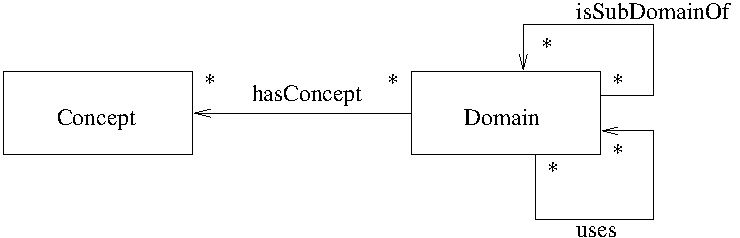
\includegraphics[scale=0.5]{img/domain}
    \caption{Semantic Structure of Domain}
    \label{domain}
  \end{center}
\end{figure}

Any other class will be a specialization of Domain and thus inherits the associations of domains such as �sub� and �uses�.
The class of Engineering Methods (see Figure \ref{engmethod}) is a specialization of the class Domain.
Thus Engineering Method inherits the subdomain relation and the relation to Concept.
Additionally, an Engineering Method is established in the context of (zero,) one ore more Domains,
it has Tools which support the Method and pragmatics for applying the Engineering Method where the
pragmatics are described by a Process (cf. [AR 00]).
\begin{figure}[htbp]
  \begin{center}
    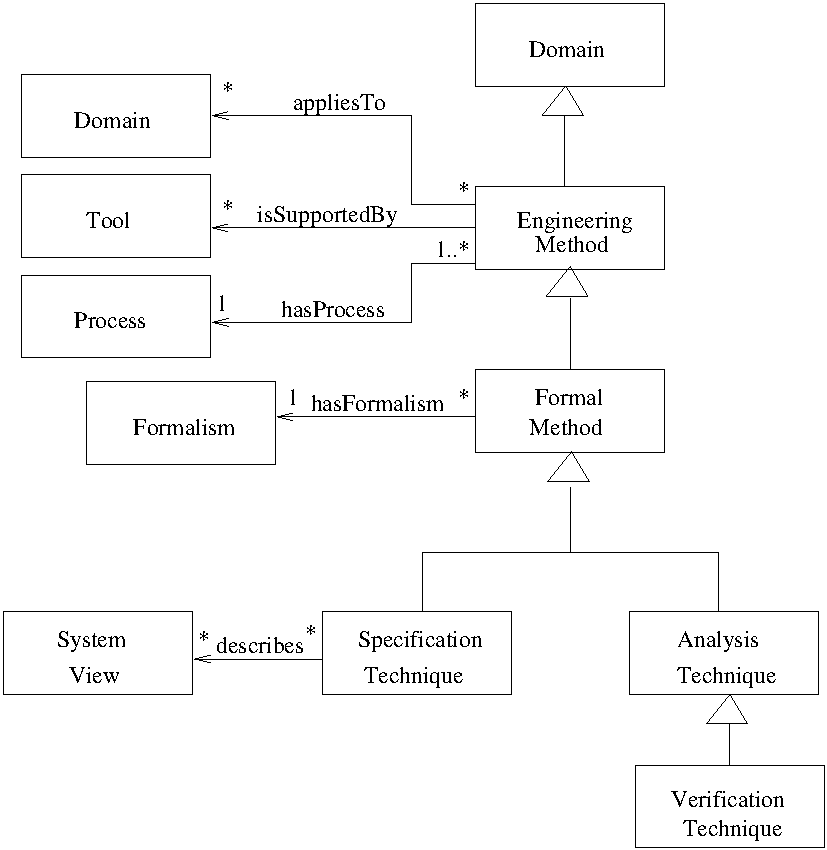
\includegraphics[scale=0.5]{img/engmethod}
    \caption{Semantic Structure of Engineering Method and Formal Method}
    \label{engmethod}
  \end{center}
\end{figure}

The class Formal Method (see Figure \ref{engmethod}) is a
specialization of Engineering Method with the particular feature that any instance of Formal Method is
based on a Formalism. Formal Methods are classified into Specification and Analysis Techniques;
Verification Techniques are a subclass of Analysis Techniques (cf. [CW 96]). Any Specification Technique
serves to specify some system views such as the data view, functional behaviour, concurrent behaviour,
performance view etc.

\begin{figure}[htbp]
  \begin{center}
    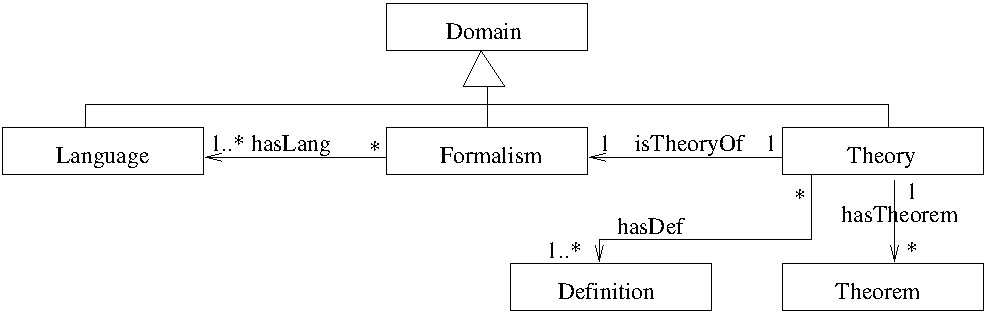
\includegraphics[scale=0.5]{img/formalism}
    \caption{Semantic Structure of Formalism}
    \label{formalism}
  \end{center}
\end{figure}
The class Formalism (see Figure \ref{formalism}) is also a specialization of the class Domain.
A Formalism has one or more associated Languages and one Theory consisting of Definitions and Theorems.
\MarginComment{JGS: ``language'' doppelt?}
Any Language (see Figure \ref{language}) has several language Language Constructs, a Classification such as natural, functional,
object-oriented or real time language (cf. [ACM 98]), and may be supported by some Tools. Moreover, any
language possesses a Language Definition consisting of a Syntax and possibly of one or more Semantics.
We specialize languages into Programming, Specification, Logical Languages and possibly other kinds of languages
which are not represented here.
\begin{figure}[htbp]
  \begin{center}
    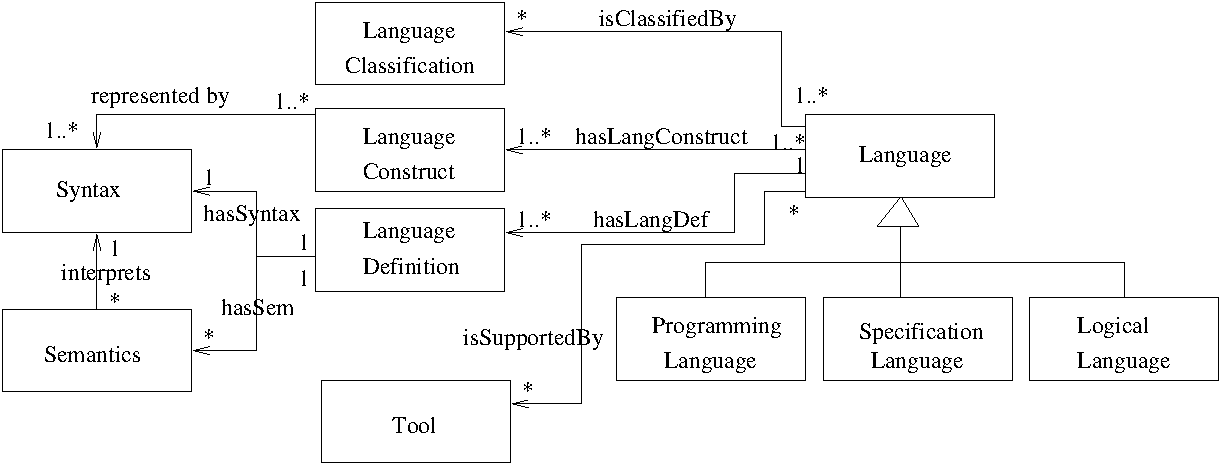
\includegraphics[scale=0.5]{img/language}
    \caption{Semantic Structure of Language}
    \label{language}
  \end{center}
\end{figure}
\end{Paragraph}
\end{Section}

\begin{Section}[Title={Systematic Construction of Ontologies},Label={Systematic_Construction_of_Ontologies}]
\begin{Paragraph}
%\subsection{Systematic Construction of Ontologies}
\label{sco}
For constructing ontologies of particular courses in the area of formal methods we proceed as follows:
\MarginComment{JGS: Sie meinen eigentlich ``previous subsection'',
  obwohl ``subsection'' zugegebenerma{\ss}en h{\"a}sslich klingt. So ist es
  aber uneindeutig.} 
We base the ontology of the course on the general model of formal methods as outlined in the previous section.
In a first step, the general model is extended by those new abstract concepts of the course which are not yet
covered by the general model. The second step consists in constructing object diagrams of the specific ontology
of the course according to the extended general model.
We give an example for this procedure by describing (part of) the ontology of the course �
Foundations of System Specifications� which is held regularly at LMU Munich. This course presents
formal techniques for specifying and refining complex data structures, state-based systems and reactive
systems. The underlying formalisms for data structures are algebraic specifications based on the language
CASL; for state-based systems these are model-oriented specification techniques based on the language Z.
The specification of reactive systems is taught by using Lamport�s Temporal Logic of Actions. In the following
we present the ontology for the specification of data structures and state-based systems.
In a first step the class diagram of Language is extended by Z and CASL which form two new subclasses
\MarginComment{JGS: Schreiben Sie ``figure'' oder ``Figure'' (uneinheitlich)}
of Specification Language (see figure \ref{languageext}).
\begin{figure}[htbp]
  \begin{center}
    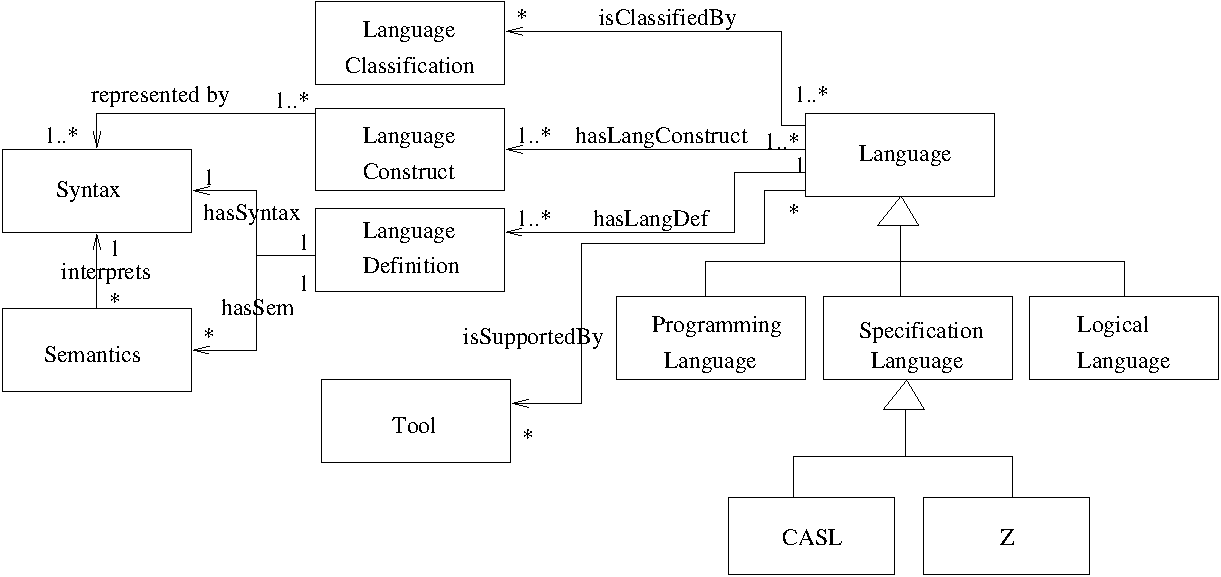
\includegraphics[scale=0.5]{img/languageext}
    \caption{Extension of the model by the languages CASL and Z of the course}
    \label{languageext}
  \end{center}
\end{figure}

\MarginComment{JGS: Besser \mbox{``CASL 1.0''} mit Abstand?}
The specific instance of CASL in the course is the version CASL1.0 (see Figure \ref{casl}).
It is classified as specification language; its language constructs are partitioned into basic specifications,
structuring constructs, architectural constructs and constructs for specification libraries.  CASL has formally
defined syntax and semantics; its tool suite consists of parsers, theorem provers and pretty printers (not detailed here).
\begin{figure}[htbp]
  \begin{center}
    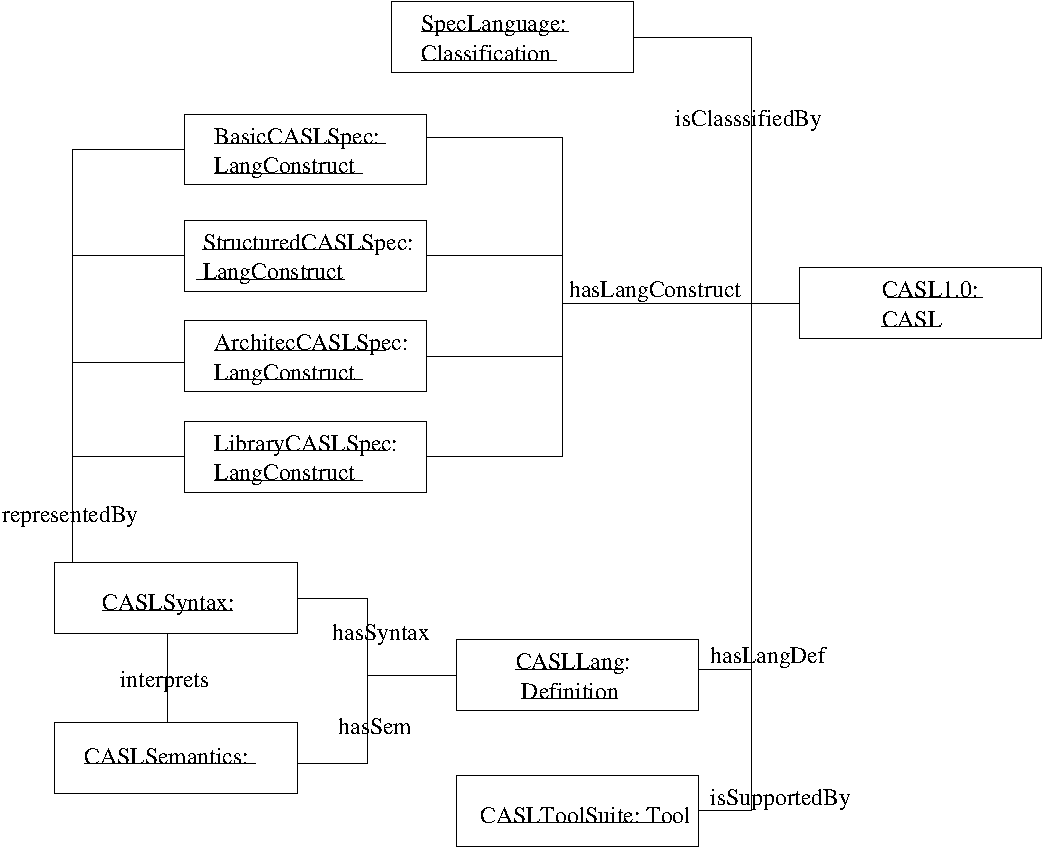
\includegraphics[scale=0.5]{img/casl}
    \caption{Ontology for CASL 1.0}
    \label{casl}
  \end{center}
\end{figure}

The specific instance of an Algebraic Specification Formalism of the course (called FSDAlgSpecFormalism) uses basic facts
about Signatures, First-order Logic and Universal Algebra for explaining the associated Algebraic Specification Theory
where different notions of refinement and their main properties, and a translation from executable specifications to the
functional programming language SML are presented (see Figure \ref{gdseformalism}).
\begin{figure}[htbp]
  \begin{center}
    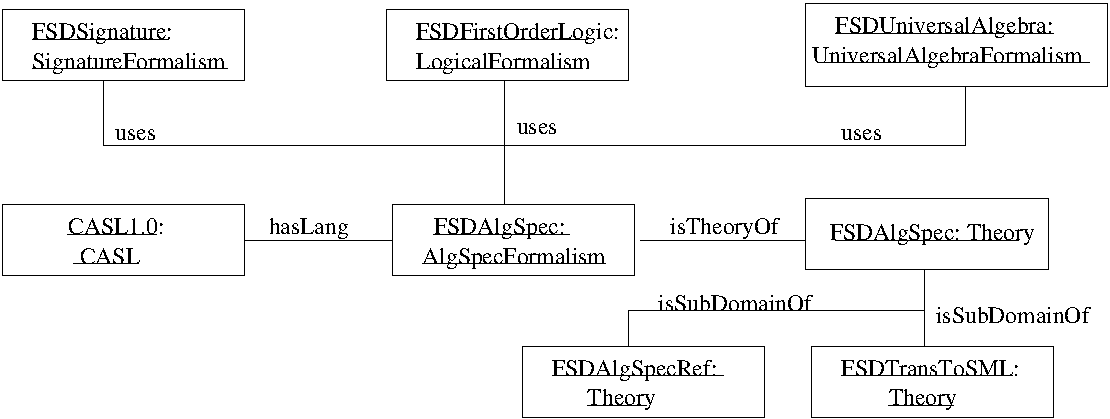
\includegraphics[scale=0.5]{img/gdseformalism}
    \caption{Ontology for the Alg. Specification Formalism of the course}
    \label{gdseformalism}
  \end{center}
\end{figure}
The instances of the ontology are prefixed by  �FSD�
since they refer to those notions and theorems of a formalism of a theory which are presented in this course.
The particular approach of the course to formal development of algebraic specifications is shown in figure \ref{gdseformalism}.
Algebraic techniques are used in the context of data specification and the development of functional programs.
The chosen development  process (the pragmatics) is stepwise refinement.

%References
%[ACM 98] ACM Computing Classification System [1998 Version],
%http://www.acm.org/class/
%[AR 00] E. Astesiano, G. Reggio: Formalism and method. TCS 236, 2000, 3-34.
%[CW 96] Edmund M. Clarke and Jeannette M. Wing: Formal Methods: State of the Art and Future Directions, ACM Computing Surveys 28 (4), 1996, 626-643.
%[KCHDBKS 01] P. Kogut, S. Cranefield, L.Hart, M. Dutra, K. Baclawski , M Kokar, J. Smith: UML for Ontology Development, 2001.
%[SMB 97] B. Steffen, T. Margaria, V. Braun: The Electronic Tool Integration Platform: Concepts and Design. Int. Journal on Software Tools for Technology Transfer (STTT) 1, 1997,  9-30.
\end{Paragraph}
\end{Section}
\end{Section}

% conclusions -- B. Krieg-Brueckner
\begin{Section}[Title={Conclusion: Experiences and Future Developments},Authors={BKB 030304},Label=s71]
\begin{Paragraph}
%\input{conclusion.tex}
%\section{Conclusion: Experiences and Future Developments}
\label{Conclusion}
\end{Paragraph}
% evaluation - an example lecture -- M. Roggenbach
\begin{Section}[Title={Evaluation: An Example Lecture},Authors={M. Roggenbach},Label=s72]
\begin{Paragraph}
%\input{experiences.tex}
%\subsection{Evaluation: An Example Lecture}
\label{Evaluation}
\RevisedBy{BKB not yet; sollte evtl entfallen}

%\Authors{M. Roggenbach} % baut seinen abstract aus

The two semester course \TECS (\Underline{Te}chniques for the
development of \Underline{C}orrect \Underline{S}oftware) provides a
gentle introduction to formal methods for software development. It
deals with sequential as well as with reactive systems, using the
algebraic specification language \CASL{} \cite{CASL/Summary} and the
process algebra \CSP{}, e.g.~\cite{roscoe98}, respectively.  On the
tool's side, the theorem prover Isabelle and the model checker FDR
play central roles. Besides simple exercises explaining single
concepts, the TeCS problem sheets also includes more complex tasks
like specifying a family game (Nine Men's Morris) in \CASL{}; verifying
a simple interpreter within Isabelle/HOL; modelling a file system in
\CASL{} at both the requirements and the design level; proving the
refinement relation between these two specifications in \HOLCASL{}.

%This should be subsumed by previous sections:
%
%To present courses like \TECS within the \MMiSS project, a markup
%language \MMiSSlatex has been developed, which consists essentially of
%a collection of \LaTeX{} style files. These style files provide
%semantic annotations for sustainable development, and create an
%adequate presentation in situations where standard \LaTeX{} is not
%sufficient. For example, a style for lecture slides produces a uniform
%format together with a consistent, configurable color scheme --- see
%the example slide in Fig.~1 --- and a variety of additional features, such as
%hyperlinks, animations, and interactive invocation of
%applications. Such features are not available in DVI. Therefore
%\MMiSSLaTeX produces \pdf. Semantic annotations are implemented as
%newly defined \LaTeX{} commands. This way, authors can write usual
%\LaTeX{} first (e.g. to produce slides for a lecture rather quickly),
%and add semantic annotations later.

\begin{figure}[htbp]
\begin{center}
% 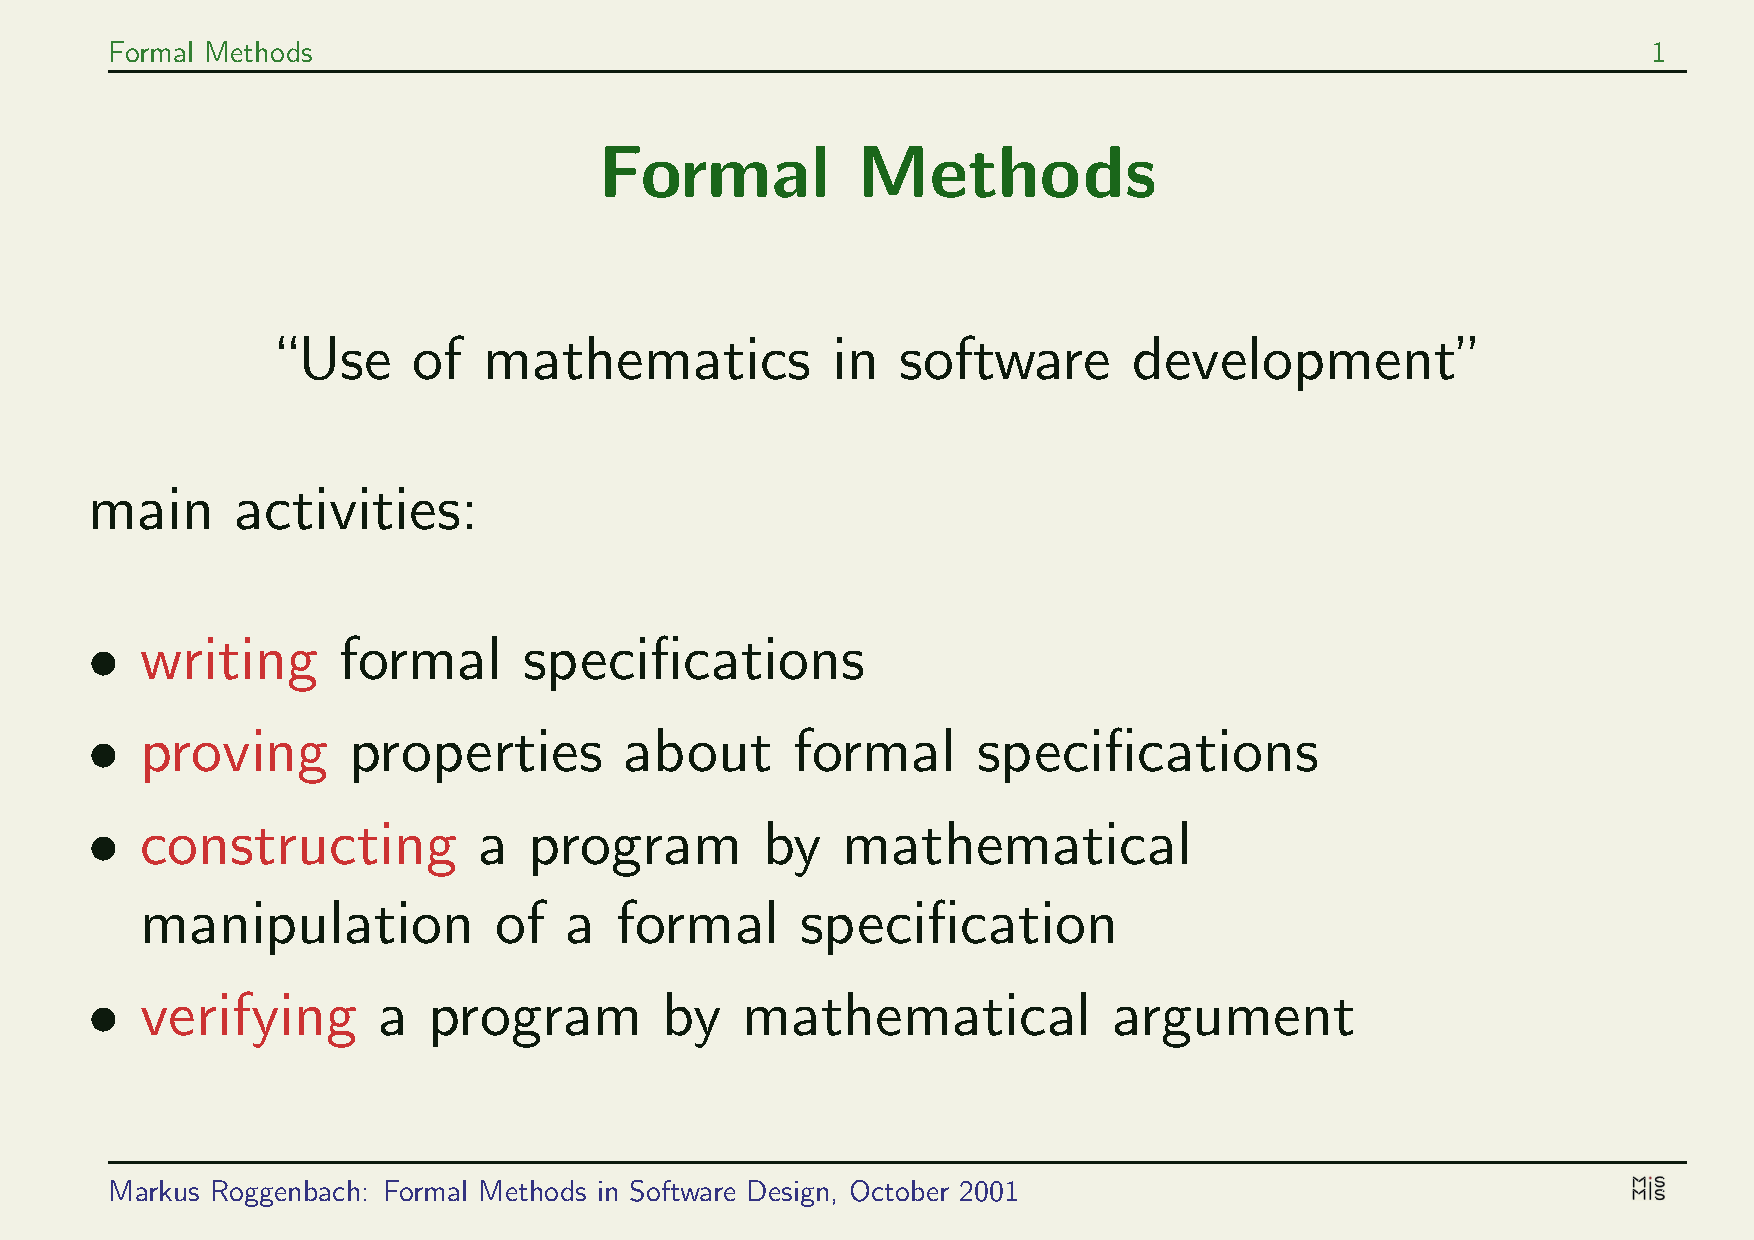
\includegraphics[width=\textwidth]{img/tecs-slide}
\caption{A sample slide of TeCS}
\label{fig:tecs-slide}
\end{center}
\end{figure}

Presenting \TECS{} using the presentational part of \MMiSSLaTeX{} has been
quite successful:
%
\begin{enumerate}

\item For the \emph{author}, the overhead to produce course material
within the \MMiSSLaTeX{} format is neglectable compared to another
presentation system.

\item Besides the usual benefits of a computer based presentation like
`no slide confusion', the \MMiSSLaTeX{} integration of tool
demonstrations in the slides encourages the \emph{teacher} to vivify
the lectures by live demonstrations on the computer.

\item The \emph{students} are fond of the
\begin{itemize}
\item the readability 
\item the consistent markup, and the
\item download-friendly PDF-filesize 
\end{itemize}
of the slides.

\end{enumerate}
%
It should be mentioned that these positive results also arise from a
cautious usage of computer based presentations: about half of the
course material has been taught in `classical style' using a
blackboard. A poll among the students of \TECS{} gave the result that
this is an optimal mixture.
\RevisedBy{BKB not yet; muss noch ueberarbeitet werden}
\end{Paragraph}
\end{Section}

%\Authors{BKB 030304}

\begin{Section}[Title={Summary.},Label=s73]
\begin{Paragraph}
%\subsubsection{Summary.}
To summarise: if you want to 
\begin{itemize}
\item  develop transparencies, lecture notes, complete courses
  levels of detail
\item  work on the board, with transparencies, interactively with tools
        interaction levels
\item  embed mathematical formulae, programs, etc. 
        \LaTeX{} formulae, tool interface
\item  manage e.g. English and German documents in parallel
  variants
\item  publish complete and consistent {\~a}packages{\`O} 
        versions, configurations
\item  (partially) re-use the transparencies of a colleague
        re-use, sharing, views
\item  be made aware of the changes made by your colleague
        change management
\item  agree with your colleague on a  uniform terminology
        ontology
\item  have support for sustainable development
\end{itemize}
then this project will have some solutions for you.
\end{Paragraph}
\end{Section}

\begin{Section}[Title={State of the Project and Future Developments},Label={Future_Developments}]
\begin{Paragraph}
%\subsubsection{State of the Project and Future Developments}
%Smaus wrote, BKB continues:
The project has made good progress during its first two years. Many
lectures have been converted to the initial \LaTeX{}-oriented input
format, with good quality output as overhead transparencies in
PDF-format. This material is now awaiting further coordination and
refinement, as well as semantic interlinking 
via an ontology and using development graphs
in the repository. The Development Manager, and other editing and
authoring tools, 
have been made available in a first version.

... are well under way towards completion.
...

%       As the tools have been under continuous development while
%       lectures were already given at the participating universities, it was
%       decided to opt for a special \LaTeX{} style as input format for lecture
%       slides.  Many lectures have been converted to this style, resulting in
%       high-quality output in the form of overhead transparencies in
%       PDF-format. We have received several requests by colleagues not
%       directly involved in the projects to make this style publicly
%       available.


The system is gradually introduced, over the duration of the
project, into the normal teaching activities of the project partners.
However, as the open source model is used and teaching materials
and tools are to be made freely available, a much greater national and
international take-up is expected. To assist this, a \MMiSS
Forum is has been founded with German, international, and industrial
members, to evaluate the emerging curriculum and assist its
development and distribution; 
you are welcome to join\footnote{http://www.mmiss.de}. 
The Advisory Board advises the
project from a scientific as well as an industrial perspective, with a
view to future applications.  To go with the planned deployment at
universities, a number of well-known German companies have already
expressed, through the various industrial contacts of the project
partners, an interest in measures for further in-house training.

...
\end{Paragraph}
\end{Section}
\end{Section}

\begin{Section}[Title={Acknowledgement},Label={s75}]
\begin{Paragraph}
%\section*{Acknowledgement}
We are grateful to the members of the Advisory Board, 
M. Kohlhase (Carnegie-Mellon University, Pittsburgh),
V. Lotz (Siemens AG, M{\"u}nchen), 
H. Reichel (Technische Universit{\"a}t Dresden), 
W. Reisig (Humboldt Universit{\"a}t  Berlin), 
D.T. Sannella (University of Edinburgh), 
and M. Ullmann (BSI [Federal
Institute for Security in Information Technology], Bonn), for their
advice, and to G. Russel for his help with the manuscript.
%% be carefull, the \end{Section} is in the included file

%       % evaluation - an example lecture -- M. Roggenbach
%       \input{experiences.tex}


% bibliography
\bibliographystyle{plain}
\bibliography{doc}

\tableofcontents{}
\end{Paragraph}
\end{Section}

\end{Package}
\end{document}

